\ifsvnmulti
 \svnkwsave{$RepoFile: lyapunov/dailyBlog.tex $}
 \svnidlong {$HeadURL: svn://zero.physics.gatech.edu/siminos/lyapunov/dailyBlog.tex $}
 {$LastChangedDate: 2019-05-11 10:46:34 -0400 (Sat, 11 May 2019) $}
 {$LastChangedRevision: 6862 $} {$LastChangedBy: predrag $}
 \svnid{$Id: dailyBlog.tex 6862 2019-05-11 14:46:34Z predrag $}
\fi

\chapter{Daily blog}
\label{c-DailyBlog}

\begin{bartlett}{
Je ne veux pas travailler\\
Je ne veux pas dejeuner\\
Je veux seulement oublier\\
Et puis je fume
            }
\bauthor{
\HREF{http://www.youtube.com/watch?v=MBoTRF2aK4s}
{China Forbes - Thomas M. Lauderdale (Pink Martini)}
    }
\end{bartlett}

\renewcommand{\ssp}{x}
\renewcommand{\vel}{\ensuremath{v}}   % state space velocity

% \section{Lyapunov vectors \KS}

\bigskip\bigskip

\noindent
{\color{red} The latest entry at the bottom of this blog,
the last page of the pdf file}
\bigskip\bigskip

% For a novice's guide to bloggery, see \refchap{sect:guide}.
To compile the whole thing or only chunks of it,
comment/uncomment \\
the \texttt{includeonly} line in \texttt{inclOnly.tex}

\bigskip\bigskip

This section of the blog is a general discussion.
\refChap{sect:LyapKS} deals specifically with the
\KS\ calculations.



\begin{description}

\item[2011-02-26 Predrag] Moved Lyapunov stuff to
    \refchap{s:LyapunovVec}.

\item[2011-10-05 Predrag] Moved H\'enon stuff to
    \refchap{c-Henon}.

\item[2011-02-22 Predrag]
So far the gap between us and Kazzanism way of thinking is as huge
as the distance from her to Kazzahstan.
Maybe start EVO group meetings?

\item[2011-02-23 Evangelos]
I would love to be able to use EVO but I've
    failed, both in the office and at home. I will arrange to meet
    physically with Kazz \etal, include you
    through EVO?

\item[2011-02-23 Predrag]
There is also a new multi-video service from Skype (paid service), not
sure whether it is comparable to EVO (EVO is real good for projection of
your presentation on other people's seminar screen).

Anyway, go talk to him - they'll have to learn quite a bit before the
collaboration would lead to something, but it would be great if we can
get together - potentially a serious step forward in (confined)
turbulence

\item[2011-03-02 Kazz] Let's start the discussion
 Monday 2011-03-07 at 13:30 (07:30 Atlanta time) at the Institut des
 Syst\`emes Complexes, 57-59 rue Lhomond, Paris.

\item[2011-03-02 Predrag] Kazz, please download
\HREF{http://evo.caltech.edu/evoGate/}{EVO.caltech.edu}, see whether you can
figure out how to use it - some notes are
\HREF{http://www.cns.gatech.edu/colloquia-seminars/AudioVisual.html}
{here}. Designed for scientists, it's better than skype if you want to
share presentations.

\item[2011-06-28 Evangelos]
There are many things I do not understand from my discussion with Kazz,
so I will wait for his notes with more details.

%\item[2011-06-28 Predrag] If Kazz is really going to write a paper, it
%would be very useful if he could learn subversion... Any chance you can
%check svn is installed on his laptop, then walk him through svn checkout
%(your GT account). If it works, I'll get his account processed by KGB,
%but it is really not worth my time unless I know he can use it...

\item[2011-08-09 Predrag] For comments to Takeuchi and Chat\'e\rf{TaCh11}
\emph{Can the inertial manifold be captured by unstable periodic
orbits?}, see [2011-07-21] entry, \refsect{sec:TaCh11}.

\item[2011-07-25 Kazz]
I am also a bit confused by not ordered time lines in the blog...

\item[2011-07-25 Predrag 2 Kazz]
Glad to oblige, but would be better if a question is answered pages
later, just because answer was typed at a later date? We who use subversion
always check the new edits using subversion diff, so we catch
edits anyplace in the blog...

\item[2011-12-01 PC to Jim Yorke] I agree with you - why attach any names
to equations? I like the thing referred to as ``Kaplan-Yorke dimension''.
Do you have a more descriptive name for it?
Cheers \& red socks forever

\item[2011-12-01 Jim Yorke to PC] The Kaplan Yorke Dimension is a formula
involving Lyapunov exponents. So we called the KY Dimension. No -- just
joking. We called it the Lyapunov Dimension. Logical?

\item[2011-12-01 PC to Jim Yorke] \emph{Who is the 2000th person who
invoked Lyapunov's name in vain?} Poor Lyapunov. He is a surname, not
concept, but his name gets attached to zillion things he had nothing to
do with.

There is something called ``Lyapunov equation'' which actually is in his
thesis, at least for the strictly contracting fixed point case.

Then there things like ``Lyapunov Covariant Vectors'' that he has nothing
to do with in any imaginable way which yield a ``physical dimension'' of
attractors of PDEs such as Kuramoto-Sivashinsky and Landau-Ginzburg. That
DOES NOT count Lyapunov exponents, it counts non-hyperbolically connected
``Covariant Vectors'', and seems to give a number roughly twice the KY
dimension.

So I'll stick to calling the KY dimension  ``Kaplan Yorke dimension'', and
leave poor Russian aristocrat out of this.


\item[2008-02-28 Predrag] \refRef{ginelli-2007-99} might offer an
intelligent way to evolve a `covariant' (?), co-moving, non-orthogonal
{\jacobianM} eigenvectors frame. See \refexer{exer:stabComoving} for
further references.

\item[2013-01-07 Kazumasa to Predrag and Evangelos]
It is a good opportunity for us to discuss how we continue our
project on \po s, Lyapunov vectors and effective dimension.

The problem we've faced for these years is that neither Evangelos or
myself have sufficient time to make active progress in this project.
Since the project is still at an initial stage where we are groping
for clues and answers (at least in my view), we may need at least one
person who can devote most of his/her time to it.

Given this situation, I'm wondering if you or Hugues can find a
student or a postdoc for the project (and other related topics).
Hugues found this idea reasonable. He says that he can possibly have
a student, but it depends on the result of a grant application that
he will receive this spring.

I'd like to know what you think of the idea and if you are interested
to have your present/future student/postdoc join the project.

\item[2013-01-11 Predrag]
I have asked one of our 1. year graduate students, Gu Qie, to join
our project on \po s, Lyapunov vectors and effective dimension. He is
a Beijing University undergraduate, and so far has all A's after the
first semester here, so it might work out, one never knows. He would
be totally dependent on Evangelos and Kazz codes to get started. He
is committed 3 credit hours/week (1/4 of his course load) fully to
this project.

\item[2013-02-14 Predrag to Kazumasa and Evangelos] Our student Qi Ge
has vanished for about a month until I accidentally collided with him
on the same astral plane this afternoon. We had a long discussion
about the project. He says he understands your papers but does not
understand what the project is. I have asked him to write down what
he got out of my verbal description of the project, so we can start
helping him to focus on the project. I have also explained to him
again that unless we get updates from him at least twice a week, I
will assume that he is not doing anything, we have no way to know
what to help him with, and then there is no point in doing the
project. There is no substitute for elbow grease...

Kazumasa, please do not 'send' Qi Ge programs, put them into
repository, as a subdirectory of directory siminos/kazz/

\item[2013-02-15 Kazumasa to Qi Ge and Predrag]
I put my code and README at siminos/kazz/code/.
Please find my comments on the coding in the Students Log Chapter.
As I announced, Hugues is now visiting me until 27 February.
We are discussing what is interesting to measure / think about in the project
 and plan to make an updated todo list in the blog.

\item[2013-02-16 Predrag]
Where does Kazumasa
\HREF{http://www.dynamicalsystems.org/ma/ma/display?item=455}{work}?

\item[2013-02-21 Kazumasa]
Predrag, you are the first (and so far only) person who found this
online article and gave me a sign. I am delocalized over real and
\textit{in silico} worlds..! (mainly out-of-equilibrium stat. mech.
probed by liquid-crystal convection)

\item[2013-04-16 Predrag]
This is probably useless, but I have saved in ChaosBook.org/library
Nichkawde\rf{Nichkawde13} {\em Optimal state-space reconstruction
using derivatives on projected manifold}.

\item[2013-05-31 Ruslan]
My student appears to be quite good at programming, so I can ask him to
write code for calculating CLVs at the \rpo s of \KS.

\item[2013-06-11 Predrag]
Yes, please ask him to do it - if two students do it independently it
is good for us, as the code can be then applied to different research problems,
first \KS, Navier-Stokes next.


\item[2013-06-11 Predrag]
Gave up on Qi Ge's project, asked him to find another adviser.
Discussed with him the Evangelos write-up in the appendix of
\refref{SCD07}, which he believed was wrong, because the tangent
vectors have to be small, not of unit magnitude. He is not learning
fast enough, me thinks...

\item[2013-06-27 Predrag] Asked \XD\ to consider this project.
He is reading up on it before deciding whether to join.

\item[2013-07-11 Predrag] Xiong (sung as Sean, as in
    \HREF{http://www.youtube.com/watch?v=0t1_usmB30s}{agent 007}) is on
    board, and studying the material. I'm hopeful, because his first
    two questions were like a sharp finger poked into my ribs: he found
    ChaosBook sections on
    \HREF{http://chaosbook.org/paper.shtml\#invariants} {Floquet
    theory} and \HREF{http://chaosbook.org/paper.shtml\#stability}
    {{\PoincSec} \jacobianMs} confusing. Well, I do not like them
    either - they are confusing.

\item[2013-08-19 Sara A. Solla] Last night I dreamt of traffic cops
that would stop and fine chaotic drivers. I saw them stopping someone
and I intervened - how did they establish that the driver was
chaotic? Had they computed Lyapunov exponents? Did they know whether
it was real chaos or non-normal chaos?


\item[2013-09-14 Predrag]
Last but not least: Congratulations! and enjoy the honeymoon. I'm of
course a bit worried, because the last time this happened, my
collaborator Ashley Willis went on a honeymoon, and then I did not
hear from him for over a year. But he's back and working again now :)

\item[2013-09-27 Predrag] Went to Dubrovnik which is full of Japanese
    newlyweds on honeymoon, but did not see Kazumasa anywhere.

\item[2013-09-27 Predrag] Gave up on \XD\ organizing out Skype
meeting, had Skype Summit with Ruslan Davidchack and
Daniel Crane, agreed on the battle plan for coming months. This is
the only current project for Ruslan, Daniel and \XD. A very brief
summary (very mangled, please edit):

\begin{enumerate}
  \item Daniel proceeds with computation of {\cLvs} for individual
      \rpo s; do perturbations of one \rpo\ stay in the physical
      manifold spanned by other ones?
  \item Need to reduce $\On{2}$ (slice? fundamental domain?)
  \item Daniel will help \XD\ get up to speed.
\end{enumerate}

\item[2013-10-29 Predrag] The elders have produced a lovely
{\em To do list},
\refsect{sect:ToDo}. Daniel and \XD, keep us posted at least once
a week about your progress on what we agreed to look at first :)

\item[2014-01-17 Predrag] Let me summarize Xiong Ding achievements so far.
I find calculation of {\cLvs} from long time limit of
Lyapunov vectors (computed from
the long time limits of
singular values and singular vectors
of (\jacobianM$\transp{)}\times($\jacobianM)) unnatural; {\cLvs} are eigenvectors of \jacobianM.
Xiong Ding has implemented three methods:
\\
(1) Lyapunov vectors method of Ginelli \etal\rf{ginelli-2007-99}.
\\
(2) The periodic Schur decomposition of
Bojanczyk~\etal\rf{Bojanczyk92theperiodic}.
As far as I know, the first direct calculation of {\cLvs} (Floquet,
as the orbit is periodic) directly from \jacobianM, all 30
eigenvalues and eigenvectors to the machine precision.
\\
(3) A much faster (not iterative) method of Granat and
Kagstrom\rf{GranatK06}, which gives him all Floquet eigenvectors and
Floquet exponents to the machine precision, at least for a short periodic
orbit.

If it all works out, one can toss out Ginelli \etal. Now, do
click on
\YTlink{chaosbook.org/videos/XiongShadowing1/XiongShadowing1.html}
and ponder what such orbits tell us about the physical dimension of
\KS.

\item[2014-01-26 Predrag] I realize that some of my colleagues use this
    word, but let's check what it means according to dictionaries:
    \begin{tabbing}
     spurious \=  Lacking authenticity or validity in essence or origin; not genuine; false \kill
      % \> for next tab, \\ for new line...
        \> based on false ideas or bad reasoning \\
        \> of falsified or erroneously attributed origin \\
        \> plausible but false; ``spurious inferences'' \\
    \end{tabbing}
A spurious relationship is a mathematical relationship in which two
        events or variables have no direct causal connection, yet it
        may be wrongly inferred that they do, due to a coincidence.

        No
        Floquet and/or {\cLvs} that we compute are
        `spurious',
they are exact and reproducible to the machine precision. Moreover, for
large $k$ they are sines and cosines. Saying `spurious' usually means that due to
computational difficulties one sees some eigenvalues that are not there, what one
sees is an artifact of imperfect computation.

Distinguishing between `physical' and `unphysical' eigen-directions is not much better -
`physical' is an over-abused term. I think we should give them names that reflect
what we mean. My suggestion for now is to call them
`entangled' vs. `transient' eigen-directions.

\item[2015-10-02 Predrag] More on the
\HREF{https://www.ias.edu/ias-letter/2015/mcdougall-latin}
     {meaning of ``spurious''}:
``\emph{spurius}, an ancient Latin term for a child born to illicit sex,
or to an unknown father.''
``Nor did they call him spurius, which they typically associated with
more serious kinds of illicit or illegal sex, such as the child of a nun
or priest, or the child of adultery or incest.''

\item[2014-03-01 Predrag]
\phantomsection\label{2014-03-01PC}
It is getting confusing, with all these \eqva, \po s, \rpo s, and \reqva.
Should we define {\em prime orbit?}
{\em prime cycle?} to mean the set of periodic points that is left
after the time and spatial symmetries have been quotiented out?


The idea of checking whether difference vectors
between nearby ergodic trajectories lie in the space spanned  by the
physical {\cLvs} is natural for the infinite time ergodic explorations
of \refref{ginelli-2007-99}, but too crude for the \po\ theory. The first
uncalled-for nuisance is computing {\cLvs} from Lyapunov vectors. Finite
time Lyapunov vectors require introduction of a norm, something that
dynamics does not care about or need.
Xiong Ding has shown how to compute directly the {\cLvs} (here known as the Floquet
vectors) for \po s, at least the short ones, with no Lyapunov vectors intermediate
step.
Next,
the notion of `nearby' points on a strange attractor also seems to
need a notion of distance, but what we are actually checking is that
the local neighborhood of an ergodic trajectory on the attractor
is spanned by the set of its physical {\cLvs}. We only need
to determine an integer, the dimension of the physical space, an integer
that should be intrinsic to dynamics and invariant under smooth coordinate
transformations. Breaking that invariance by imposing an arbitrary norm on
the \statesp\ only gets in the way.

We propose to densely populate the strange attractor with unstable \po s.
So what we are checking is
whether the strange set in the neighborhood of any periodic point is
spanned by its set of {\cLvs}.

Even though it seems wrong, let's define a distance between points on
a pair of trajectories embedded in the strange set, using a norm such
as the L2 norm, $\norm{\ssp}^2 = \braket{\ssp}{\ssp}$,
\[
D(\ssp(\zeit_1,\gSpace_1),\ssp(\zeit_2,\gSpace_2))^2=
\norm{\LieEl(\gSpace_1)\ssp(\zeit_1)
      -\LieEl(\gSpace_2)\ssp(\zeit_2)}^2
\]
Using $\Group$-equivariance we can always eliminate one of the group
transformations, so this distance depends on 2 times and $N$ relative
phases $\{\gSpace^{(1)},\cdots,\gSpace^{(N)}\}$. We set $N=1$ in what
follows. The `times' $\{\zeit_1,\zeit_2\}$ are not the single, dynamical
`clock' time, but parametrizations of the two finite trajectory segments
$\ssp(\zeit_1)$ and $\ssp(\zeit_2)$; they could be L2 arclengths of the
curves, or any other monotonic parametrization of the curves. We'll take
these segments to be segments of a single prime \po, or a pair of \po s.
The goal then is identify close points in the ergodic attractor (close
recurrences) and check whether their difference vectors lie in the
inertial manifold, as spanned by the Floquet vectors of either of the two points.

The minimal distance satisfies the $2+N$ extremal conditions
\[
\frac{\partial~}{\partial s}
D(\ssp(\zeit_1,1),\ssp(\zeit_2,\gSpace))^2= 0
\]
where variation with respect to phases $s=\gSpace$ yields the usual
slice condition, and variation with respect to time yields
\[
\braket{\sspRed(\zeit_1)
      -\sspRed(\zeit_2)}{\vel(\zeit_1)} = 0
\,.
\]
Do I need to do this for every point on orbit $\sspRed(\zeit_1)$? Looks
like it; you move along $\sspRed(\zeit_1)$ and for each point
check the locally shortest distances to trajectory
$\sspRed(\zeit_2)$. Then check the 2nd derivative to identify local minima, and keep
only those close passes that are closer than some small distance. Every difference
vector that is longer has to be thrown away, as it connects points on a curved
manifold and is thus necessarily traversing the full dimensionality of
the embedding space. This needs
yet another criterion for what is a `small' distance. Do not like this at all -
there should be some differential condition computable from each individual
\po, we are interested in $D\to 0$ neighborhood,
so this is a statement about the infinitesimal neighborhood.

We usually quotient time invariance by arbitrary transverse global
(sets of) {\PoincSec s}. This is different: not only is the local slice
hyperplane chosen to minimize distance, also the local {\PoincSec} has
to minimize distance. That means we are using the information along
entire \po s, not merely their periodic points in a given global
{\PoincSec}.

If we are lucky, that will go away, and a single {\PoincSec} will
suffice. The idea is this difference vectors are transported around a
\po\ by the Floquet matrix of the linearized flow; they can get stretched and
skewed, but the dimensionality of the space they span cannot change...

\item[2014-11-13 Xiong] I created a Bibtex entry\rf{DCTSCD14}
  for the manuscript we
  are going to write about the physical dimension of the inertial manifold.

\item[2014-11-16 Predrag to Xiong] Please
\begin{enumerate}
\item create a skeleton of article \refref{DCTSCD14} in folder
\texttt{dimension/} now, and start writing it, following the {\bf
[2014-09-23 Kazz to Xiong and everyone]} outline. Do not wait for any
further revolutionary developments - the senior co-authors, who have more
experience in such matters than you, have deemed the results that we have
now worthy of publishing, and that is that. Two months of not acting on
this is ... I do not know what to say. Do not even dream of postponing
the article to 2015 or 2025.
\item Change macros in \texttt{schur/} to {\em SIAM J. Appl. Dyn. Syst.}
macros, and the reorder the physics into front part of the article. Add
no new material to it - that will be for another publication. You have
let this totally completed article sit fallow since {\bf [2014-07-09]}. I
do not know what to say. Do not even dream of postponing the article to
2015 or 2025.
\end{enumerate}

Reuse some variant of this text in above articles and your thesis:

{\em Turbulent fluid flows are in principle $\infty$-dimensional
dynamical systems. For dissipative flows, including presumably (the
$\$1M$ question) the Navier-Stokes flows, after the initial transient a
turbulent flow settles into a steady-turbulence state. In the \statesp\
this strange attractor, or `inertial manifold' is of a 	relatively low
dimension. This fact has motivated many 	reduced-order models for
fluid turbulence, none of them able to describe the actual turbulence. We
take a different path, and propose to tile this highly curved, nonlinear
manifold with a collection of finite-dimensional linearized
neighborhoods, each tile centered on one of our numerically exact
solutions of Navier-Stokes equations.
}

                                                        \toCB
Recently, Yang~\etal\rf{YaTaGiChRa08} have undertaken a detailed
statistical study of the dynamics of linearized stability eigenvectors
(what they call `{\cLvs}') for $1D$ \KS\ and complex Landau-Ginzburg
systems. The eigenvectors corresponding to the leading (in)stability
exponents are highly non-normal. They find that for a fixed size system
{\cLvs} can be cleanly separated into two sets: (a) the finite, fixed
number of `entangled' or `physical' eigenmodes whose pairwise angles
can be arbitrarily small (\ie, perturbation along one can easily
propagate along the others), and (b) the rest, the approximately
orthonormal set  of (infinitely many) strongly contracting, `unphysical'
eigenmodes, along which perturbations simply fall back into the inertial
manifold. If the numerical resolution of the PDE integrator is doubled,
all extra eigenvectors fall into the `unphysical' set. Thus we have, for
the first time, an operational definition of the dimension of an inertial
manifold, in contrast to the early rigorous, but non-constructive bounds
on dimension of inertial manifolds for several such dissipative
PDEs\rf{constantin_integral_1989}. As a moral tale, we note that this
explicitly computable physical dimension is about twice of the previously
widely accepted heuristic guess, the Kaplan-Yorke
dimension\rf{KapYor79,FKYY83}.

Their work was made possible by recent algorithmic
advances\cite{ginelli-2007-99,WoSa07} which enabled them to compute
reasonably accurately large numbers of `{\cLvs}', the eigenvectors of the
linearization of flow centered on an ergodic trajectory. While effective
in predicting the dimension of the inertial manifold by evaluating statistical
averages along the trajectory, this methods yields no intuition about the
geometry of the attractor. We propose instead to determine the physical
dimension by carrying out such analysis on recurrent flow solutions. The
hierarchies of unstable \po s, together with their Floquet vectors,
provide a rigid skeleton by which both the local hyperbolicity and the
global geometry of the inertial manifold is embedded into system's
high-dimensional \statesp.

To this end, graduate student Xiong Ding and PI have
developed~\rf{DingCvit14} a new `periodic Schur decomposition' algorithm
for computation of \emph{all} Floquet vectors and exponents of (relative)
periodic orbits to machine precision.
\begin{figure}[h]
  \centering
  \text{(a)}
  %\includegraphics[width=0.10\textwidth]{KSppo1State2}%\hfill
  \text{(b)}
  %\includegraphics[width=0.41\textwidth]{vectorPPO1MarginalFrame}%\hfill
  \text{(c)}
  %\includegraphics[width=0.36\textwidth]{KSspectrum2}
  \caption{
    A pre-periodic orbit in \KS\ system with periodic boundary condition,
    $ u_t+ u_x u +u_{xx}+u_{xxxx}=0\,,\quad x\in [0,L] $.
    (a) Evolution of the orbit in 4 prime periods.
    (b) \Statesp\ evolution of the two marginal Floquet vectors along one
    period this orbit.
    (c) The real parts of Floquet exponents (`Lyapunov exponents') of
    this orbit.
            }
  \label{fig:ppo1StateVectorSpectrum}
\end{figure}
\refFig{fig:ppo1StateVectorSpectrum}\,(a) shows a typical short
pre-periodic orbit of \KS\ flow as time evolution (vertical) of the \KS\
field $u$ (color coded) defined on a spatial periodic domain (horizontal).
\refFig{fig:ppo1StateVectorSpectrum}\,(b) shows that the evolution of two
marginal directions along this orbit, computed by our algorithm,
accurately align everywhere with the velocity field and the group tangent
directions, as they should. The power of the algorithm is demonstrated by
\refFig{fig:ppo1StateVectorSpectrum}\,(c) which gives the \emph{full
spectrum} of expansion rates of stable/unstable directions of this orbit;
the inset shows the Floquet exponents of the 8 physical dimensions. We
also have the full set of eigenvectors at any point along this orbit; it
is their dynamics that establishes the separation between the physical
and unphysical dimensions. While the previous numerical methods can
compute a dozen or so eigenvectors, our algorithm is capable of computing
them all. This is a highly non-trivial step forward for our program, as
the entries in Jacobian matrices whose eigenvalues we are computing
easily range between moderately expanding (here $\sim 10^3$) to insanely
contracting (here $\sim 10^{-2642}$).

With this robust algorithm at our disposal, we intend to first chart the
entire inertial manifold for \KS\ on a small periodic
domain~\rf{DCTSCD14}. Due to the `hyper-diffusive' $\nabla^4$ term in its
linearized spectrum, \KS\ has a very stiff built-in spatial length scale.
In order to make sure that the sharp separation of the physical and
unphysical modes observed so far is not an artifact of this intrinsic
\KS\ scale, we are currently writing fast code for the $1D$ cubic-quintic
complex Landau-Ginzburg equation. This system has only Laplacian
$\nabla^2$ terms, two continuous symmetries, and much richer dynamics
(deterministically diffusing `exploding solitons'\rf{DesBra13}, \etc). If
we can show that the {\cLvs} definition of the `physical dimension' is
robust over a variety of $1D$ dissipative PDEs, we will make a brave
attempt to determine it for the full $3D$ Navier-Stokes, no modeling
assumptions. That will be much harder, as the embedding dimension is
$\sim 10^5$, and we expect the physical dimension to be in hundreds
(rather than 8, as the case in our KS on a small periodic domain,
\reffig{fig:ppo1StateVectorSpectrum}\,(c)).

If we succeed in charting out the inertial manifold by neighborhoods of
unstable \po s, and establish the physical dimensions for each, there is
potential to radically reduce the scale of fluid dynamical direct
numerical simulations: instead of integrating with $\sim 10^{6}$ global
computational elements, the integration can be done on collection of
linear neighborhood charts, each of dimension $\sim 10^{2}$.


\item[2015-05-12 Xiong] I put an example web page in
lyapunov/examples/plotFV.html
to show the Floquet vectors of \cycle{ppo_1}.

\item[2015-10-15 Predrag]
Started summary of WebEx meeting in \refsect{sect:2015-10-15}. If you have some notes,
enter them there.

\item[2015-10-25 Kazumasa]
I hope Predrag reads my emails.
{\bf [2015-10-26 Predrag]} I herby reassure you that anything sent into
my mailbox goes straight into the black hole at the center of our galaxy :)
For science, blog it.

I need to confirm the effect of the symmetry reduction on the
Floquet vectors. In the present manuscript, you wrote, below Eq.~(4),
\begin{quote}
Note, all periodic orbits and the corresponding Floquet vectors are
calculated in the full \statesp. Formula~(4) only tells how to
transform state points onto slice, but the corresponding Floquet vectors
are first transformed with the state point, and then projected onto the
slice, as illustrated in figure~3.
\end{quote}

If this is true, I would understand that the studied ``Floquet vectors"
are indeed projections, so they lose information on the components
tangent to the considered symmetry. Those components can a priori have
non-zero values, even for Floquet vectors other than the marginal one
corresponding to this symmetry. Then this projection also affects the
angle shown in Fig.~4. Is this correct?

I'd also like to know if the value of $\theta$ in Eq.~(4) is chosen globally
or locally in time. In other words, the question is whether you
transform each orbit onto the slice at each instant of time
independently, or you determine the value of $\theta$ using information at
a specific time t and transform the orbit with the same $\theta$ for the
whole period. If $\theta$ is fixed, then the condition in Eq.(3) is
satisfied only at the specific time you use for determining $\theta$ (and
then I don't understand why a relative orbit makes a closed loop). In
contrast, in order that Eq.~(3) always holds, it seems to me that you
need to adjust the value of $\theta$ at each time step.

\item[2015-10-26 Xiong]
Yes. The symmetry tangent component is gone for each Floquet vector after
projection.  Predrag prefers to use name ``coordinate transform" because
we can regard the symmetry direction as a moving coordinate so if we
record the component in this direction before projection, then we can
recover the original vector.

For the measured angle. I guess I understand what you mean. There are 2
approaches to measure the angle. First, Floquet vectors are only rotated
to the slice but not projected. In this case, we still need 8 Floquet
vectors. Second, Floquet vectors are rotated and projected. Since the
symmetry tangent components is gone, in principle, the measured angle
should be larger than that of the first approach. But I found that they
are almost the same. I prefer the second approach because they are the
true Floquet vectors in the symmetry reduced \statesp.

For $\theta$ in Eq.~(4), yes, they are state dependent. Different points
in the \statesp\ will be rotated to slice by different angle. I
calculate the orbit in the full \statesp\ first, and then for each
point on it, I calculate the corresponding $\theta$, this $\theta$ will
be used to rotate the state point onto slice and will also be used to
rotate Floquet vectors.

\item[2015-10-26 Predrag]
For me ``projection'' from $d$ dimensions to $d'$ dimensions means that
you have thrown away $d-d'$ coordinates. Symmetry reduction by \mslices\
is not a projection - for $\SOn{2}$ it is a local `moving frame'
coordinate change where one coordinate measure where the state is along
the compact phase angle direction (along the `fiber'), and the $d\!-\!1$
coordinates tell you where the state is in the ($d\!-\!1$)\dmn\ slice
hypersurface (for us, usually tiled by locally good enough hyperplanes).
No coordinate is thrown away, the phase is kept track of by the
`reconstruction equation'.

The distances between any two states are measured \emph{in the slice}. For
\rpo s nothing happens along the group tangent direction - the Floquet
multiplier is 1, so there is no contribution to distance from there, if
you study recurrences. That is \emph{the whole point}, that's why we had
to reduce symmetry, there is no sensible way known to us to measure
distance between two wursts (AKA $N$-tori) in the full \statesp. Symmetry
reduction recovers the notion of \emph{recurrence}, which is what Xiong
is measuring. It's hard to figure out what recurrence would mean if one
were to compare states with different phases along the group symmetry
coordinates.

Did Xiong and I answer your questions?

Do not look at me like that. Go bug Cartan\rf{CartanMF}.

\item[2015-10-27 Kazz]
Thanks. I understood what you did.
I perfectly understand the importance of symmetry reduction and agree that it is a coordinate transform to the state (dynamical variables), in the sense Predrag clarified: combining the information of the phase, one can indeed recover the original coordinates of the orbits. However, I still suspect that it may be NOT the case of the Floquet vectors, because they are first calculated with the full \statesp, then PROJECTED to the slice. Here the component tangent to the symmetry direction is LOST, as Xiong clearly answered above. Of course this doesn't cause a problem if the obtained Floquet vectors before projection are already decoupled, specifically, if the marginal mode corresponding to the symmetry has the Floquet vector perfectly tangent to this direction and all the other vectors are perfectly perpendicular to it (so their component in the tangent direction is zero). If this is the case, we need to clarify it in the paper. If not, we (at least I) need to think carefully about the meaning of the ``Floquet vectors'' after slicing.

If the vectors are not decoupled, I strongly suggest to use the first
method Xiong explained, in which the Floquet vectors are only rotated to
the slice but not projected. Actually I prefer this method even if the
vectors are perfectly decoupled, because I believe we should avoid the
projection anyway. In addition, in this way the number of the physical
modes can be kept the same throughout the paper.

\item[2015-10-26 Xiong 2 Kazz]
The shadowing numerical investigation is done in the symmetry
reduced \statesp. I are not measuring angles in the full
\statesp. Everything is reduced to the slice including the \Fv s
before collecting shadowing incidences.
The validity of the projection process is justified in
\eqref{eq:variation_full_slice} and \eqref{eq:relation_jacobian1}.
I think it is too long to explain the projection details, so I only
use one illustration figure in the paper.

So basically, I am trying to get the lower bound of the dimension
of the \inm\ of the symmetry reduced \statesp. And we assume that
quotienting out the continuous symmetry only decreases the dimension
by one, but keeps the essence of the system unchanged. So in this way,
we can infer the dimension of the full \statesp.

This is the logic in my mind when writing this part.
Now I understand
why you ask whether the angle changes or not after projection.
My intention is not trying to measure some angle in the full \statesp.

Reread the paper again. Yeah, I think a lot of logic is missing.
That's true. We need to make it logically sound.


\item[2015-10-26 Xiong]
I think studying the dimension of the \inm\ of the symmetry reduced
\statesp\ bears more merit than study the full \statesp.
Because usually when we take on a dynamical system, the first step
is to reduce the continuous symmetries, at least for SO(2).
The procedure mentioned in the paper is resulted from the work flow
of \KSe. I take a post processing method to reduce the symmetry only
because the symmetry reduced integrator is not well
justified, and also all relative \po s are initially found in the
full \statesp\ and \Fv s are calculated in the full \statesp.

But, that's true, the description in the paper is somewhat misleading.
Could I update some parts of it tomorrow ?

\item[2015-10-27 Kazz]
You don't understand my point. I'm saying it is not evident that your ``Floquet vectors'' in the symmetry reduced space can be regarded as the eigendirections of the corresponding Floquet multipliers, if they have non-zero component in the symmetry-tangent direction in the full-space descriptions. If they are indeed the true Floquet vectors in the reduced space, they should have vanishing component in the tangent direction even in the full space. So I asked you to check this. Also, though I perfectly agree that we should use the slicing for the state variables themselves and should rotate the Floquet vectors accordingly, I don't see any advantage in throwing away their symmetry-tangent component artificially.

\item[2015-10-27 Xiong]
Just as I said, the justification of the symmetry reduced
\Fv s is given in \eqref{eq:relation_jacobian1}, which relates the
Floquet matrix in the full \statesp\ and that in the slice. We are not
throwing away symmetry-tangent component artificially, but it is
required by the definition of the slice
\eqref{eq:slicecondition} intrinsically. As far as I'm concerned,
as long as we are working in the slice, any symmetry tangent
components vanish naturally.

\item[2015-10-27 Kazz]
In terms of \eqref{eq:relation_jacobian1}, my question is whether the vectors obtained by equation (9.82) with $|\delta x\rangle$ being the Floquet vectors of the full-\statesp\ are indeed the eigenvectors of the matrix in left-hand side of \eqref{eq:relation_jacobian1}. Do you check this with your data?

\item[2015-10-27 Xiong]
You can have a look at \reftab{tab:floquetM1}, which list the
Floquet exponents in the full \statesp\ and those
calculated directly in the slice for the same
orbit. For \Fv s, I show how well the projection works
for the two-mode system
on the next page of formula \eqref{eq:relation_jacobian1}.

I mention \eqref{eq:relation_jacobian1} twice because the relation is
manifest in it.
\begin{equation}
  \hat{\jMps}(\sspRed(\zeit_2),\sspRed(\zeit_1))\hat{h}
  (\sspRed(\zeit_1))g(-\theta_{1})=
  \hat{h}(\sspRed(\zeit_2))g(-\theta_{2})\jMps(\ssp(\zeit_2),\ssp(\zeit_1))
  \,.
\end{equation}
For relative periodic orbits,
$x_{p}(0)=g_{p}x_{p}(T_{p})$, also we have
$\sspRed(\zeit_1)=\sspRed(\zeit_2)$ and $g(-\theta_{1})g_{p}=g(-\theta_{2})$.
Relation in \eqref{eq:relation_jacobian1} becomes
$\hat{\jMps}(\sspRed(\zeit_2),\sspRed(\zeit_1))\hat{h}
(\sspRed(\zeit_1))g(-\theta_{1})
=\hat{h}(\sspRed(\zeit_2))g(-\theta_{1})J_{p}(\ssp(\zeit_2),\ssp(\zeit_1))$,
so covariant vectors are also transformed by
$\hat{h}(\sspRed(\zeit))g(-\theta)$. To sum up, if $e_{i}(x(t))$ is a
covariant vector associated with a (relative) periodic orbit at
point $x(t)$ in the full
\statesp, then $\hat{h}(\sspRed(\zeit))g(-\theta)e_{i}(x(t))$ is
the corresponding covariant vector at position $\sspRed(\zeit)$ on the
slice, here $x(t)=g(\theta)\sspRed(\zeit)$.

The above notations look cumbersome. So I want to add a
light version of \eqref{eq:relation_jacobian1} in the paper.

\item[2015-10-27 Kazz]
Ok, the result in \reftab{tab:floquetM1} indeed suggests that the
symmetry tangent component is vanishing, at least for this specific
orbit. But, then, nothing would change for the Floquet vectors by this
``projection'', right? (btw, don't use the word projection, because it
means you do lose information outside the projected plane) So I'd suggest
not to remove that vanishing component. Don't misunderstand, this doesn't
mean we don't use the symmetry reduction, since the state variables are
always sent to the slice and so are the Floquet vectors, always. I'm just
claiming the ``projection'' makes the story complicated in vain.

\item[2015-10-27 Xiong]
My concern is that if we do what you suggest, then the orbit is in
the slice, but the \Fv s are still in the full \statesp, so
this tangent bundle is not well defined, although your suggestion
is easier to accept for readers.

I will ask Predrag today for his opinion. I should make him happy.:)

Predrag is on travel. I think as long as the reader can accept the
fact the slice is a one-dimension-less hyperplane, then we are fine.
Symmetry reduced state points has dimensionality $d-1$, the vectors
should have the same dimensionality; otherwise, we choose not to use
slice at all.

\item[2015-10-28 Kazz]
Thinking the phrase ``this tangent bundle is not well defined", maybe I
see what you mean. You are concerned about the definition of the angle
between the difference vector (in $(d-1)$-dimensional slice) and Floquet
vectors, if the latter is expressed in $d$-dimensional full \statesp,
right? Indeed. Then how did you compute the angles in
\reftab{tab:floquetM1} for full-space Floquet vectors?

I think every reasonable reader can accept that "the slice is a one-dimension-less hyperplane", and this is not my point. I am pointing out a potential danger of your projection (not the slice! we must use the slice). If we can show, hopefully in a mathematical way, that all Floquet vectors (except the one corresponding to the symmetry) live in the sliced hyperplane even without that projection (in other words if their symmetry-tangent component is zero), I'm perfectly fine. Anyway, I'd first like to know how you computed the angles in \reftab{tab:floquetM1} for full-space Floquet vectors.

\item[2015-10-28 Xiong]
First, I need to say: YES, definitely they have. \Fv s in the full
\statesp\ are not perpendicular to symmetry tangent component. So what ?
so you are concerned that that if the information of of this component is
lost, the symmetry component of the difference vector is left in the air,
right ?

But let's
think it in this way. Initially we have 30 \Fv s, each of which has
30 components. Now after transformed to slice, one of them vanished so
we are left with 29 vector, each of which has 29 components. This set
of vectors span the full tangent space of the symmetry reduced \statesp.
Can the symmetry component of the difference vector be expanded
by this set of NEW \Fv s ?

\item[2015-10-28 Kazz]
I see, Floquet vectors do have the non-vanishing symmetry-tangent component. My whole concern was I was not sure about the meaning of the projected Floquet vectors. Are they eigenvectors of something? The existence of the non-vanishing symmetry-tangent component indicates that, in the full-\statesp, if you remove that component by hand, that vector wouldn't serve as the Floquet vector (i.e., it doesn't give the corresponding Floquet multiplier anymore). Then in what sense the projected Floquet vectors can be regarded as the Floquet vectors? That's the whole point that I want to clarify by these discussions.

Sorry I don't understand what you want to ask me in your last paragraph. I'm also waiting for your answer on the way to compute the angles in \reftab{tab:floquetM1} for full-space Floquet vectors.

\item[2015-10-28 Xiong]
Formula \eqref{eq:relation_jacobian1} says that the projected \Fv s
are the eigenvectors of the Floquet matrix (\jacobianM) in the symmetry reduced space.

\refTab{tab:floquetM1} does not list angles. It lists Floquet exponents
of the Floquet matrix in the full \statesp\ and the Floquet exponents
of the Floquet matrix in the slice for the same relative \po.

\item[2015-10-28 Kazz]
Sorry don't understand. If I understand correctly, the formula
\eqref{eq:relation_jacobian1} shows the matrix $\hat{J}$ that gives
evolution of the projected vector $\delta \hat{x}_p$. This doesn't
necessarily say that this $\delta \hat{x}_p$ is an eigenvector of
$\hat{J}$. Can you show this?

Sorry about my misunderstanding on \reftab{tab:floquetM1}, but what is
$\theta$ there? Anyway, then, could you explain how you computed $\mu$
for the reduced-space Floquet vectors? Your estimates there were obtained
separately from those for the full-space Floquet vectors, right?

\item[2015-10-28 Xiong]
I use a notation-light version of \eqref{eq:relation_jacobian1}.
\begin{equation}
  \hat{\jMps}^t(\sspRed_2,\sspRed_1)\hat{h}
  (\sspRed_1)g(-\theta_{1})=
  \hat{h}(\sspRed_2)g(-\theta_{2})\jMps^t(\ssp_2,\ssp_1)
\,.
\label{eq:blogex}
\end{equation}
Here $\sspRed_2 = \sspRed_2(\zeit_2)$ , $t=t_2-t_1$and
$\sspRed_1 = \sspRed_1(\zeit_1)$. $\ssp_1$ and $\ssp_2$ are in the
full \statesp, and $\sspRed_1 = g(-\theta_1) \ssp_1$,
$\sspRed_2 = g(-\theta_2) \ssp_2$ are the corresponding points in the
slice. $\theta_1$ and $\theta_2$ represent the rotation angles
that transform
them to the slice.

For a relative periodic orbit, $x(0)=g(\theta_p)x(T_{p})$, which means
after period $T_p$, the end point can be rotated to the initial point
by $g(\theta_p)$. So let us take $x(0)$ and $x(T_p)$ to be
$\ssp_1$ and $\ssp_2$ in \eqref{eq:blogex} respectively. Then we have
$\sspRed_1 = \sspRed_2$ because in this case
$ -\theta_1 + \theta_p = -\theta_2$. So relative \po\ becomes \po\
in slice. Then \eqref{eq:blogex} becomes
\begin{equation}
  \hat{\jMps}^{T_p}(\sspRed_1,\sspRed_1)\hat{h}
  (\sspRed_1)g(-\theta_{1})=
  \hat{h}(\sspRed_1)g(-\theta_{1})g(\theta_p)\jMps^t(\ssp_2,\ssp_1)
  \label{eq:blogex2}
\end{equation}
Also the Floquet matrix for relative \po\ in the full \statesp\ is given
by $g(\theta_p)\jMps^t(\ssp_2,\ssp_1)$. So if $e_i$ is an eigenvector of
$g(\theta_p)\jMps^t(\ssp_2,\ssp_1)$, then multiply $e_i$ at both
ends of \eqref{eq:blogex2}, we get
\begin{equation}
  \hat{\jMps}^{T_p}(\sspRed_1,\sspRed_1)\hat{h}
  (\sspRed_1)g(-\theta_{1}) e_i=
  \Lambda_i \hat{h}(\sspRed_1)g(-\theta_{1}) e_i
  \label{eq:blogex3}
\end{equation}
We see $\hat{h}(\sspRed_1)g(-\theta_{1}) e_i$ is the eigenvector
of $\hat{\jMps}^{T_p}(\sspRed_1,\sspRed_1)$ with the same eigenvalue
$\Lambda_i$ as $g(\theta_p)\jMps^t(\ssp_2,\ssp_1)$. Here
$\hat{\jMps}^{T_p}(\sspRed_1,\sspRed_1)$ is the Floquet matrix in the slice
of a \po\ which starts from $\sspRed_1$ and end in $\sspRed_1$.

\item[2015-10-28 Xiong]
The symbol $\theta$  in \reftab{tab:floquetM1} represents the phase of
complex Floquet exponents. I have an integrator which can directly
integrate the dynamics in the slice, so I can obtain the Floquet matrix
in the slice directly, not by ``projection''. Then I compare the Floquet
exponents in the slice with that in the full \statesp, basically, to show
\eqref{eq:blogex3} is correct.

\item[2015-10-28 Kazz]
Got it. Now everything seems clear to me, thanks!

I think the whole confusion came from the term "projection", in the way different from what I thought before. The meaning of your projection is to apply the matrix $\hat{h}(\hat{x}_1)g(-\theta_1)$ to a vector, right? This is absolutely not the projection, which usually means applying a matrix
\begin{equation}
 P = \left( \begin{array}{@{\,}ccc|c|ccc@{\,}}
 1 &        &   &   &   &        & \\
   & \ddots &   & 0 &   &    0   & \\
   &        & 1 &   &   &        & \\ \hline
   &        &   &   & 1 &        & \\
   &    0   &   & 0 &   & \ddots & \\
   &        &   &   &   &        & 1 \end{array} \right).
\end{equation}
This is completely different. Now I agree what you did is legitimate. The remaining problem is that we need to give a good name to replace your term projection. Any suggestion?

\item[2015-10-28 Xiong]
Initially I use ``projection matrix'' for  $\hat{h}$
because it is singular. It transforms a symmetry tangent vector
to zero vector. So
$\hat{h}(\hat{x}_1)g(-\theta_1)$ is rotation followed by a ``projection''.
To use another name, transformation matrix, gauge-fix matrix ?
For me, ``projection'' is the best word in my mind.
If diagonalized, it is
\begin{equation}
  \hat{h} =
  \begin{pmatrix}
    0 & 0 & 0 & \cdots \\
    0 & a & 0 & \cdots \\
    & & \cdots &  \\
    0 & 0 & \cdots & b \\
  \end{pmatrix}
\end{equation}

\item[2015-10-29 Kazz]
I disagree about using the word ``projection'', mainly because it has the
specific meaning as I explained (Fig.3 of the draft also supports this
standard definition of projection by the way), which then misleads the
readers, resulting in a serious consequence about the reliability of our
results.

A question: can you recover the full-\statesp\ Floquet vectors from the
reduced space vectors plus the phase $\theta$ used to send the orbit to
the slice? If yes (I believe so, based on my new understanding), then I'd
suggest ``coordinate transformation (matrix)'' as Predrag also suggested
before. The essential difference from ``projection'' is that the latter
word usually implies that we discard the information outside the
projected plane \textit{irreversibly}. I believe it is not the case of
our Floquet vectors.

\item[2015-10-29 Xiong]
That is true. We can recover original vectors given phase $\theta$ and
a scale $\braket{t'}{e_i}$ before ``projection'' since
\[
  \hat{h}(\hat{x}_1)e_i = e_i -
  \frac{\braket{t'}{e_i}}{\braket{t(\sspRed)}{e_i}} t(\sspRed)
\]
But I cannot see the problem with this word. Apparently,
for any kind of projection, if the
``perpendicular'' part is recorded before projection, then we
can recover the original vector.

\item[2015-10-29 Kazz]
Very good. Xiong, remember, the word ``projection'' is misleading because
it has the specific meaning as I explained, which is fundamentally
different from what you do. The word has confused me a lot, who is as an
author one of the few persons who know the work best, so why can we
expect readers to understand it correctly?

\item[2015-10-29 Xiong]
Ok. I am waiting for a better word other than ``projection''. But for me,
``transformation'' is not so true either, because it gives me a illusion
that slice has the same dimensionality as the original \statesp.

\item[2015-10-29 Kazz]
Well, including the phase $\theta$, it has the same dimensionality, but I see what you mean. Predrag may have a good idea.

\item[2015-10-27 Predrag 2 Kazz]
I think elsewhere we have used term \emph{``in-slice Floquet vectors''};
could we do that here?

Let me first say that if I sound like I am sure that one should be
measuring angles between in-slice Floquet vectors rather than the full
\statesp\ Floquet vectors: I am not sure. There might be something about
keeping marginal directions that is important for the eigendirections
entanglement, something that I am missing.

But there is no doubt that in-slice Floquet vectors retain all full
\statesp\ Floquet multipliers, with exception of the marginal eginvector
whose eigenvalue is identically zero, so there is now way to measure any
length along it. You would do me a favor if you work through \texttt{ChaosBook}
ver. 14, section
\HREF{http://www.streamsound.dk/book1/chaos/chaos.html\#104/z}
{4.6 Stability of Poincar\'e return maps}.
I do use word `projection' but agree with you that we would rather not.

\item[2015-10-29 Xiong]
I am against the idea of keeping the symmetry tangent direction in
expanding difference vector which is measured in slice. But I think the
name ``in-slice \Fv s'' is cool.

\item[2015-10-30 Kazz]
Agreed about ``in-slice \Fv s'' (and agree with Predrag that the marginal
direction may potentially play a role, but the result shown in the draft
suggests that at least for the physical dimension its role is trivially
adding one dimensionality). Now I, with Hugues, start touching the draft.

Xiong, could you give me the raw data used for the figures? (i.e.,
numerical data and/or figure files that contain data) Or, are there
somewhere in the repository?

\item[2015-10-29 Xiong]
For the raw data,I probably have 100G. I need to read my script to
figure out what
statistical manipulations I have done in order to generate the data
only for figures. Sorry. I generated the figures on the way manipulating
the raw data. Please give me a little time. I will upload the data and the
Python plotting scripts I used.
The current figs are all in folder \texttt{siminos/xiong/figures/}.

Is that OK ?

\item[2015-10-30 Kazz]
Thanks. I don't need 100G raw data, but just wanted the numerical tables
used to make the figures (in other words, arrays of x and y coordinates
of the data points in the figures).

\item[2015-12-04 Kazz]
I and Hugues are exchanging the draft and comments.

\item[2015-12-09 Kazz to Xiong]
To complete the second draft,
 we would like you to answer the following questions:

\begin{enumerate}
\item
What numerical scheme do you use for integrating the KS equation? What is the time step and the cutoff wavenumber (assuming you used the quasispectral method in space)?

Xiong : Exponential time-differencing
scheme combined with RK4\rf{cox02jcomp,ks05com} is implemented. This
method is also used by Ruslan. He has some matlab code in
\emph{siminos/matlab/ruslan} folder. But I have C++ implementation.
I set $N=64$ as truncation number.

\item
Were the PPOs and RPOs found by the method explained in Predrag's SIAM 2010 paper (Appendix C), exactly?

Xiong : I believe so. Ruslan gave me the data set. I use it as initial
guesses and find RPOs and PPOs for larger truncation number.

{\bf Ruslan:} Yes, all the essential details of the search algorithm are described in that paper.

\item
What is the bias we have in the orbits detected by the used method? If I understand correctly, we detect only orbits near the attractor (which is good) and it's harder to detect orbits that are more unstable, or less frequently visited by chaotic trajectories, right? I guess the detection rate is proportional to $\exp(-\sum_i \lambda_i T)$, where the sum runs over positive Floquet exponents $\lambda_i$ and $T$ is the period. Is this correct?

Xiong : I did not try to find \po s from recurrent states, and
basically I start from Ruslan's data set. So I do not know how
the actual performance of the multi-shooting
algorithm depends on the stability of orbits.
However, from Ruslan's database, it seems more likely that
shorter orbits are more frequently found even it is very unstable.

{\bf Ruslan:} I wouldn't be so categorical in saying that we only detect orbits near the attractor.  If orbits outside the attractor existed, then this method would also be able to find them.  As to any 'bias', it is hard to say anything definite.  The only thing I can say is that the search was really exhaustive for shorter orbits.  This is simply because there are not so many of them as the longer ones.  So, majority of the shorter orbits were 'hit' multiple times.  I have recorded the number of times (field {\tt nhit} in the data structure) each orbit was detected, and these numbers are very large for most short orbits.   Even though it is generally true that more unstable orbits are harder to detect, I believe it is too simplistic to think that the relationship with Floquet exponents will be so simple.  It would indeed be interesting to analyse the correlation between the orbit instability and the number of times it was detected.

{\bf Kazz:} Thanks! Could you explain why you don't think you only detected orbits near the attractor? If I understood correctly, you had used recurrence points of chaotic trajectories as an initial guess of orbit, then adjusted the initial condition, the period, etc. to find a true orbit; is this correct? Then I thought that the found orbit is near the attractor, in the sense that nearby chaotic trajectories shadow that orbit and (are expected to) share the same instability properties.

{\bf Ruslan:} Even though the search is seeded with a close return within the chaotic orbit, the search algorithm is not restricted to stay on the attractor (or even on the inertial manifold).   So, if such orbits outside the chaotic attractor existed, then I believe they would have been detected (at least some of them).  My belief that there is nothing else 'out there' is also based on the observation that the dynamics of the KS is strongly dissipative and the region around $u=0$ (the trivial solution) is completely surrounded by the attractor.  So, I just cannot think of any other 'far away regions' where something could be happening outside of the chaotic attractor. (There is probably also an argument that can be made in terms of a suitable Lyapunov function for this system, but I'm not clever enough to think it through.)

\item
What is the value of $\Delta t$ used for the local Floquet exponents? Numerically it cannot be the limit $\Delta t \to 0$ as described in your manuscript.

Xiong : For integration of the orbits, I use $\Delta t \sim 0.001$
slightly different for each orbit. However when calculating \Fe s,
I use $\Delta t' = 5\Delta t$, so basically, every 5 time steps I
record the short-time Jacobian.

\item
Do you know any literature about the TPH as you describe in the manuscript? I am in particular wondering if the claim "one consequence of partial hyperbolicity is that the angle between these two subspaces are bounded away from zero" is proved and/or supported by past work.

Xiong : This is a headache for me because It is hard to read pure
mathematical paper. Here, I follow Pesin's note\rf{Pesin2004} on
discussion of partial hyperbolicity. See section 2.2 in this note
and Proposition 2.1 proves
"one consequence of partial hyperbolicity is that the angle between these
two subspaces are bounded away from zero". For TPH, sorry, it is
totally fabricated by me.


\item
Hugues and I agree that perhaps we have to be more careful about the claim that ALL the orbits share the same structure of crossing of $\lambda_i(t)$. Isn't it related to the bias we have in the detection of orbits? In other words, do atypical orbits (less frequently visited by chaotic trajectories, more unstable, but still part of the skeleton of the attractor) also share the same crossing structure? Can you check this?

Xiong : The orbits used in the statistics are the first 200 shortest
PPOs and RPOs. I did not discard any of them. It is hard to say whether
the dataset is complete or at least dense because we do not have a
complete description of the geometry of the strange attractor, namely,
the symbolic dynamics. But I think Ruslan's code is effective enough
to capture all possible short \po s no matter whether the \po\ is
atypical or not.
The shortest PPO $\cycle{ppo}_{10.25}$ looks like not embedded in the
attractor, and is quite unstable.

{\bf Ruslan:} We cannot say that the data set is complete, but I believe it can be said with high confidence that, based on the exhaustive nature of the search for orbits with $T < 100$, the number of orbits which remained undetected is very small.

{\bf Kazz:} I then believe that short orbits near the attractor are most probably detected, but I'm not so sure about orbits located far away from the attractor, where the hunting was not even tried (I guess such regions/orbits exist, right?). Moreover, I feel a bit strange that the crossing structure of $\lambda_i(t)$ is shared even with orbits that have instabilities very different from those of chaotic trajectories. Xiong, could you tell me (1) the largest value of the 1st Floquet exponent among your 400 orbits, and (2) the smallest value of the 8th Floquet exponent (in other words the last physical exponent) among the same 400 orbits?

{\bf Xiong:} The largest 1st \Fe\
is $0.327911586426$ coming from shortest $\cycle{rpo}_{16.3148}$.
The smallest value of the 8th \Fe\ is $-0.527435116415$, the 19th
$\cycle{rpo}_{54.76}$.

{\bf Kazz:} Thanks! Could you give me time series data of the instantaneous Floquet exponents (as in Fig.1(b) of the draft) of $\cycle{rpo}_{16.3148}$?

{\bf Xiong:} I uploaded it in folder \texttt{dimension/Fig1/} file
\texttt{rpo1expand.dat}. It is a 30 x 3200 matrix, the same format as
FVexpand1.dat.  Row $i$ contains time-series for $k=i$.

{\bf Kazz:} Thanks. It's fun to see that the largest exponent has a crossing during a very short time window, only barely, and the partner is the 6th exponent.

\item
About your Fig. 2(b), how many points from each orbit did you use to construct the histogram? If multiple points were used, how did you choose their phase along the orbit?

Xiong: As I said, when calculating \Fe s,
$\Delta t' = 5\Delta t \sim 0.005$. For example, for
$\cycle{ppo}_{10.25}$, I measure angles at 2000 points on this orbit.
For longer orbits, there should be more points.
What does phase refer to ? Real \Fv s are unique. Complex conjugate
pairs are always counted in the same subspace.

\item
What is the time length of the chaotic trajectory used for the shadowing analysis? Did you use a single chaotic trajectory for all shadowing events for all orbits, or you used several chaotic trajectories?

Xiong : I used a single chaotic trajectory to obtain the shadowing
events for a single RPO or PPO, so it is quite long.
For different RPO/PPO, I restart the
code, so the chaotic trajectory starts from different places.

\item
About your Fig.4(c)(d), what do you get if you only use the minimum angle during each shadowing event, instead of using all points during the shadowing?

Xiong : I think I did similar calculation before, see \refFig{fig:disAngScatter_localMin}.
Although data points are fewer, the structure does not change too much
(compare  \refFig{fig:disAngScatter_localMin} with  \refFig{fig:disAngScatter_ppo4}). Note,
these two figure have not removed the ``bad'' points.

\item
Can you produce a figure like \reffig{fig:ppo34ppo191} of the blog for shadowing to ppo$_{33.39}$? This is to put as a part of Fig.4, so it would be nice if the size (especially the aspect ratio) of the figure is the same as the other panels.

Xiong : I will do it. But \reffig{fig:ppo34ppo191} is shadowing between two PPOs. What I will
do is shadowing between PPO and chaotic trajectory.

\item
How does your Fig.4(c) look like if you add data for $k=9,11,17,21,25$ to your Fig.4(c)? Do we
still see a V-shape like in \refFig{fig:disAngScatter_ppo4}
and \refFig{fig:disAngScatter_localMin} in the blog?

Xiong : If I add data for $k=9,11,17,21,25$ in Fig.4(c), then it looks like a mass,
too many points and overlapping. I will show it to you soon.

For V-shape, I guess you are referring the
slight dip in Fig.4(d), not the V-shape that in \reffig{fig:disStructure}
(``bad'' points have been removed by me).

\item
About Fig.4(c)(d), can you produce similar figures for ppo$_{33.39}$? In addition, what do you get if you use all shadowing events you have, mixing data for different orbits?

Xiong: Yes, I will show the figure for ppo$_{33.39}$ soon.
Mixing data for different orbits does not sound interesting to me because shadowing only gives
information about local structure. Mixing them may smooth out some particular geometrical
character near some specific orbit. I will do it if you insist.

\item
Give me data points used for:
(1) spectrum of Floquet/Lyapunov exponents for ppo$_{10.25}$, rpo$_{16.31}$, and chaotic trajectory, like in Fig.1(a) but WITHOUT taking into account the degeneracy. \\
(2) Fig.1(b) + similar time-series for $k=11,12,13,14$. \\
(3) Fig.2(b), Fig.4(a)-(d).

Xiong :
(1) $\cycle{ppo}_{10.25}$ is contains in \emph{dimension/Fig1/ppo1.npz}. In it, variable
`fe' is a 62x1 vector ( WITHOUT taking into account the degeneracy). See
\emph{dimension/Fig1/fig1.py} for how to load the data. Folder Fig1, Fig2 and Fig4 contains
the data for the plots in the draft.
Are you sure you also need $\cycle{rpo}_{16.31}$ ? It is not mentioned in the draft.

(2) It is contained in \emph{dimension/Fig1/FVexpand1.dat}.
This file contains a 30x2000 matrix. Row $i$ contains time-series for $k=i$.
See \emph{dimension/Fig1/fig1.py}

(3) They are contain in folder Fig2 and Fig4 already. The python script the these folder
help you load and plot the data.

\end{enumerate}
If there is anything unclear, don't hesitate to ask me, instead of trying to understand it by yourself.

\item[2015-12-09 Kazz to all coauthors]
About the order of the authors, I guess we all agree that Xiong should be the first. For the rest, how about the alphabetical order?

\item[2015-12-11 Kazz to Xiong]
Thanks Xiong for the answers, I will consider them and revise the draft.

\item[2015-12-11 Kazz to Ruslan]
Could you complement Xiong's answers to my questions 2 and 3 above? Thank you!

\item[2015-12-11 Ruslan to Kazz]
Answered above.

\item[2015-12-11 Kazz to Ruslan \& Xiong]
Thanks Ruslan! I replied to your answers 3 and 6. I also have a question to Xiong in the reply 6.

\item[2015-12-15 Kazz to Ruslan]
Ok, I didn't know that even $u=0$ is approached by chaotic trajectories. Then I intuitively agree with you that probably all orbits are ``near'' the attractor, though I also understood that we don't know how to corroborate this belief theoretically.

\item[2015-12-15] Ruslan to Kazz
Actually, the chaotic attractor stays away from $u=0$, so I think I might have misled you with my comment that the chaotic attractor surrounds the origin.  So, maybe I should not be so categorical in my assertion that there is nothing else outside the attractor.

\item[2015-12-15 Kazz to Ruslan]
Ok, thanks.

\item[2015-12-28 Kazz to Xiong]
I am waiting for some data and figures I had asked, listed below.
Please prepare the data in text format instead of Python binary
 (I'm not used to Python).
\begin{enumerate}
\item
Spectrum of Floquet/Lyapunov exponents for rpo$_{16.31}$ and chaotic trajectory, without taking into account the degeneracy (asked in the above 13). Yes, I'd like to show the spectrum of an rpo and a chaotic trajectory as well (of course they will be mentioned in the new text). Knowing that rpo$_{16.31}$ is somewhat unusual (most unstable in the database), perhaps rpo$_{34.64}$ may replace rpo$_{16.31}$ (but rpo$_{16.31}$ or any other rpo is still okay).
\item
A figure like figure 9.15 of the blog for shadowing to ppo$_{33.39}$ (asked in the above 10). Yes, what I want is also a shadowing to the chaotic trajectory.
\item
Raw data for your Fig.4(a)-(d), and figures like Fig.4(c)(d) for ppo$_{33.39}$, in text format.
\end{enumerate}
I also have a few questions and remarks:
\begin{enumerate}
\item[3]
I found that your fig2.py does NOT reproduce your figure 2(b)(c).
Specifically, the abscissa are different.
Which is the correct one?
If the data contained in ab.npz is incorrect, provide me with the correct data
 (in text format).
\item[4]
Concering Fig4.(c)(d), I agree that mixing up different orbits would not make sense. So such an analysis must be performed for each orbit. For how many orbits did you carry out this analysis (excluding false recurrence points (called ``bad'' points by you))? I guess you did so at least for ppo$_{33.39}$ and rpo$_{34.64}$, but did you also try other orbits?
\end{enumerate}

\item[2015-12-28 Xiong to Kazz]
I will send you the text data in email because it is a little large.
fig2.py and the corresponding data are updated. Fig.2 in the draft is
correct. Sorry about the mistake.

For Fig4(c)(d). I tried all orbits in \reffig{fig:disAngScatterN32_2},
but the data is massed up expect $\cycle{ppo}_{33.39}$
and $\cycle{rpo}_{34.64}$. I think \reffig{fig:disAngScatterN32_2}
is quite representative if the `bad' points are ignored.
You can try $\cycle{ppo}_{33.39}$ using data
that I will send you. The tendency does not change.

\item[2016-01-28 Kazz to Xiong]
We are finalizing our turn, but found a serious problem. About Fig.2, bottom panel, when I changed the range of the y-axis, I found some hidden noise (or signals), continuing up to the vanishing angle... see this for the leftmost two distributions:

\begin{center}
 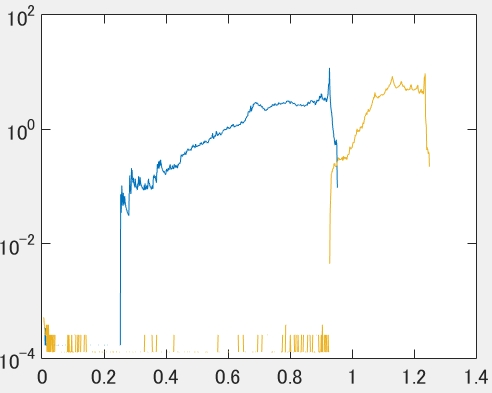
\includegraphics[width=0.5\hsize,clip]{angleDisNoise}
\end{center}

Could you explain what it is? If you believe it's noise, explain how this kind of noise could be made.

\item[2016-01-28 Xiong to Kazumasa]
I already noticed this tiny distribution at the bottom
the first time I used my new database. The problem is
that some new calculated \Fv s does not converge for a few
orbits (probably less than 10).
I think the fraction is so small, so I just
removed it intentionally to hide this
unsatisfactory part instead of picking out the bad \Fv s.
I must made a mistake that I uploaded the
unrefined data.

\item[2016-01-29 Kazumasa to Xiong]
I see... but what makes me worried is that the noise part seems to be flat and continue up to the vanishing angle. If it is due to an imperfect convergence, shouldn't we get a distribution deformed from the true one? I'd like you to identify from which orbit and at what moment the noise comes in (for a few smallest angles of the distribution with $n=8$ and 10, for example), and check if it's really due to the bad convergence.
Since we are claiming that for $n=8$ the distribution is bounded away from zero, this check is crucial. If there is an orbit for which the angle may reach zero, we need to modify our claim.

\item[2016-01-28 Xiong to Kazumasa]
OK. I will try to check. It may take 2 or 3 days. I am confident that it
will not affect our claim.
For uploading figures in svn, you first need to add the figures and then
commit.
\begin{verbatim}
   svn add nameOfFigure.png
   svn commit
\end{verbatim}
I am not sure whether this is your problem.

\item[2016-01-29 Kazumasa to Xiong]
Thanks, I guess it works. I wouldn't bother you by trying to upload an unnecessary file, but I noted this command.
Concerning the check, I then wait for news from you.

\item[2016-01-30 Xiong to Kazumasa]
The angle distribution of rpo 33, 36, 59, 60, 79, 81, 109, 114
are wired, so I suspect their \Fv s do not converge. I use a smaller
tolerrance $rtol = 1e-12$ to recalculate \Fv s. These 8 orbits
all converge and now the angle distribution slightly changes and is
within expectation.

Data in \texttt{siminos/dimension/Figs2} is updated.

\item[2016-02-01 Kazumasa to Xiong]

OK, very good... let me confirm that you didn't truncate any data in the new file. Correct?

\item[2016-02-01 Xiong to Kazumasa]
No.
Data is replaced not truncated.

\item[2016-02-01 Kazumasa to Xiong]

Unfortunately it seems to me that the data were truncated (all pdfs were cut at the density 0.02). What I wanted to know was the reason why you had the noisy signals in the previous data set and I didn't want you to manipulate the data in this way. Just give me the new, raw data (after convergence was improved) without truncating anything. If you think you don't truncate, explain why the pdfs stop at the density 0.02, while it continued to nearly 0.001 in the old data set.

\item[2016-02-01 Xiong to Kazumasa]
Wait. Let me see what is going on there.

\item[2016-02-01 Xiong to Kazumasa]
Ok. It is my mistake. The python script needs to be updated.
I uploaded the new \texttt{ab.npz}. I will send you the raw
data by email.

Thanks for pointing it out.

\item[2016-02-01 Kazumasa \& Hugues to everyone]

Please find a new version of the paper uploaded on \verb|siminos/dimension-new|, to which we both converged. We hope you will appreciate it. We believe it now really looks like a PRL! Of course, there may be room for improvement and changes, but we feel now it's almost ready for submission.

To Predrag, we would like you to check carefully what we write about Navier-Stokes and your past papers. To be specific, we want you to check the following:\\
1. Is the Navier-Stokes equations believed to have a finite-dimensional inertial manifold? (see the first paragraph of the manuscript; perhaps it depends on in which regime of turbulence we are)\\
2. Do you know any important study on the periodic orbit expansion that does NOT come from your group (and is worth mentioning in our paper)?

To Xiong, please check that all technical details in the draft are correct.

We also prepared a coverletter and a 50-word summary, both needed for the submission to PRL. These are included in \verb|coverletter.txt|.

\item[2016-02-01 Kazumasa to everyone]

I remind you that now Evangelos has the priority for edit.
So I recommend that others don't edit the manuscript yet, but your comments
 are welcome! (especially we wait for Predrag and Xiong's answers
 to our questions/requests)

\item[2016-02-01 Xiong to Kazumasa]
Thanks for the excellent improvement. I can see a substantial change in
the content of the new draft. For me, it has a new object:
physical manifold.

I have a few questions. \\
1. X-axis of Fig1(a) is $j$, should it be $j * 2\pi/L$ because I
assume that $j$ is an integer. \\
2. Regarding ``the exponential time-differencing fourth-order Runge-Kutta
scheme [20] and the spectral method'', it looks like we have two different
numerical schemes. Is it true? \\
3. For the supplementary material, should the title be changed to
``Estimating the dimension of the inertial manifold from
unstable periodic orbits'' ? \\
4. In the supplementary material, I think it is better to add the
definition of slice $<\hat{x}(t)|x_0> = 0$ and give
$x_0 = (1, 0, 0, \cdots, 0)$ because readers then know what is really
going on in formula $(S5)$.

\item[2016-02-02 Kazumasa to Xiong]

I'm happy that you like the new version. Yes, we introduced the term
``physical manifold'' to mean the manifold constructed by the physical
Floquet/Lyapunov modes.

Here are the answers to your questions:

\begin{quote}
1. X-axis of Fig1(a) is $j$, should it be $j * 2\pi/L$ because I
assume that $j$ is an integer. \\
\end{quote}
The x-axis is meant to be the Floquet/Lyapunov index, so it is integer. Therefore, $j$ is correct. Let me know if I don't understand your point.

\begin{quote}
2. Regarding ``the exponential time-differencing fourth-order Runge-Kutta
scheme [20] and the spectral method'', it looks like we have two different
numerical schemes. Is it true? \\
\end{quote}
You know this, don't you? ``The exponential time-differencing fourth-order Runge-Kutta scheme'' is about the way to discretize the time, while the spectral method is about the space discretization.

\begin{quote}
3. For the supplementary material, should the title be changed to
``Estimating the dimension of the inertial manifold from
unstable periodic orbits'' ? \\
\end{quote}
You are right, thanks! (I forgot to change it from an old title)

\begin{quote}
4. In the supplementary material, I think it is better to add the
definition of slice $<\hat{x}(t)|x_0> = 0$ and give
$x_0 = (1, 0, 0, \cdots, 0)$ because readers then know what is really
going on in formula $(S5)$.
\end{quote}
I agree (well, I guess you meant $<\delta\hat{x}(t)|T x_0> = 0$). I revised the supplementary material accordingly.
Thank you for your quick and careful check!

\item[2016-02-02 Xiong to Kazumasa]
Thanks.
I am curious about the range of x-axis in FIG1(a)
because it stops at about 18. But I have 62
exponents in the database. So I suspect we are plotting against
$j * 2\pi/L$. For the numerical method and supplementary material,
I have no problem now.

Wait for Evangelos' and Predrag's opinions.

\item[2016-02-02 Xiong]
OK. I find that only the leading part of the exponents are plotted.

\item[2016-02-03 Kazumasa to Xiong]
Yes, that's the reason. I think showing detailed structure of the spectrum near the threshold and the difference between chaotic trajectpries and periodic orbits is more important than showing the entire spectrum, which just overlaps with previously reported Lyapunov spectrum of chaotic trajectories.

\item[2016-02-05 Evangelos]
I finished with my edits of the main manuscript but I would like to read more carefully the supplementary material during the weekend.
I think that the letter was very well written and my suggested edits are optional, Xiong you can revert them if you don't like them.
There are some comments about possible clarifications that I think are needed but I didn't try to do myself because I felt there might
be objections to them, so I have left them as questions in the text (see the boyscout version).

\item[2016-02-14 Kazumasa]
I had a look at the new draft.
I tried to edit, but I couldn't figure out implicit rules for editing
(it seems to me that I must follow the way of editing which I don't know, with commands that are defined somewhere else and that I need to know to edit),
I give my comments and questions here:

\begin{enumerate}
\item
I found that ``physical'' and ``spurious'' Floquet/Lyapunov modes are rephrased to ``entangled'' and ``transient'' ones. Why is it? Since ``physical'' and ``spurious'' were used in previous publications, to avoid unnecessary confusion it doesn't seem to me a good idea to change them unless there is a strong reason for that. In particular I'm against the use of ``transient'' here because those spurious modes are not transient, defined as the usual Lyapunov/Floquet modes.

\item
About citing Oseledec's original paper, I agree it's always a good thing to cite the original one, as well as other papers that help understand the theorem.

\item
Concerning Evangelos' remark that the description of our previous results on the physical/spurious Lyapunov modes is hard to read, I'd be happy to try improving, once I am told how to edit the manuscript.

\item
Concerning Evangelos' remark in p.4 (about whether we showed the inertial manifold is fully defined in the phase space), I agree that it should be rephrased along the line you proposed.

\item
About Predrag and Xiong's comments in p.5, my opinion is the following: (1) I feel better with $\theta_p$ than $\ell_p$ to be consistent with the notation in Burak's PRL 2015 (which will be useful to understand our supplementary). (2) About the three types of orbits, I think it's better to mention these three types and then explicitly state that no periodic orbit with reflection symmetry was found in our detection method.

\item
I think it's better to abbreviate pre-periodic orbits and relative periodic orbits as we did in the previous version, simply to save the word count, and also because we do use the abbreviations to specify the orbits.

\item \textbf{(to Predrag and Xiong)}\\
As Evangelos remarked, local Lyapunov/Floquet exponents (with the limit $\tau\to 0$) are not nonsense: it is \textit{not} the eigenvalues of the stability matrix, because we use the globally-defined Lyapunov/Floquet vectors to compute these local exponents.\\
That said, Evangelos and I realized that by using the analytical expression of the stability matrix with the numerically obtained Floquet vectors, one can actually directly evaluate the local exponents for $\tau \to 0$. I think this will be a very good improvement, because otherwise our choice of $\tau=0.005$ may look arbitrary and subjective. Xiong, I know this may be painful to you, but I believe it's worth. Could you do this?

\item \textbf{(to Xiong)}
To answer Evangelos' question about the angle distribution (in p.8), could you identify the orbit and the time that gave the smallest angle in the distribution of Fig.2, and show us a histogram of the angle of that particular orbit?

\item
The footnote ``Our Floquet/Lyapunov spectrum does not include...'' was referred to multiple times, but in the current version it is cited only at the first place. I think we should keep this reference at the places I set, otherwise readers may consider that our estimate of the physical manifold is different from the previously reported one.

\end{enumerate}

\item[2016-02-15 Xiong]
For point 7 above,
I calculate local \Fe s, and the result looks the same as that of
finite time \Fe s with $\tau = 5\Delta t$.
Assume $e_i(x)$ is normalized in the following.
\begin{align*}
  \lambda_i(x) & = \lim_{\Delta t \to 0} \frac{1}{\Delta t} \ln ||J^{\Delta t} e_i|| \\
               & = \lim_{\Delta t \to 0} \frac{1}{\Delta t} \ln ||(1+A(x)\Delta t) e_i|| \\
               & = \lim_{\Delta t \to 0} \frac{1}{2\Delta t} \ln (e^\dagger_i(1+A^\dagger\ESedit{\Delta t})(1+A\Delta t) e_i) \\
               & = e^\dagger_i \frac{A^\dagger + A}{2} e_i \\
\end{align*}
For real \Fv s, $\lambda_i(x) = e^\dagger_i  A e_i$. For complex conjugate pairs,
$\lambda_i(x) = Re(e^\dagger_i  A e_i)$. This is slightly different from covariant Lyapunov vectors,
since the latter are
always real. \refFig{fig:localFEppo1} shows the result for $\cycle{ppo}_{10.25}$. Result for
$\cycle{rpo}_{16.31}$ is also obtained.
\begin{figure}[h]
  \centering
  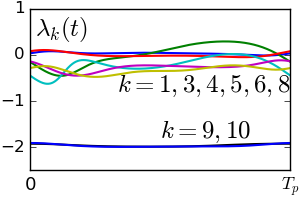
\includegraphics[width=0.6\textwidth]{localFEppo1}
  \caption{Local \Fe s of $\cycle{ppo}_{10.25}$. Compare it with the
    figure of finite \Fe s in the draft.
  }
  \label{fig:localFEppo1}
\end{figure}

For point 8 above, Evangelos thinks we need to rephrase
sentence ``tangency cannot be reached during a finite period
of time by any pair of Floquet subspaces''. I guess he is not
questioning the result.  Other phrases like
``tangency is not manifest... ", or ``tangency is not credible for
study only one orbit..." may be used.


For $\ell_p$ and $\theta_p$, I not saying we should use $\ell_p$
not $\theta_p$.
I find in the draft $L$ is used to substitute $\ell_p$, which is
problematic because $L$ is already reserved for domain size $22$.


\item[2016-02-17 Evangelos 2 Xiong] Thanks a lot for the figure
clarifying point 7! I think that this figure should be included
in the manuscript instead of the one that uses the arbitrary time
$t=5\Delta t$.

Regarding point 8, I do not have an objection about the result
or about the fact that using an ensemble of orbits is the best way
to make sense of the angle between subspaces.
The reason that I have a problem with the wording is that,
since we do numerics, we should anyway not expect that a quantity
defined to be $\geq 0$ take an exact zero value over a
numerical trajectory. On the other hand we make a statement that
sounds exact: ``tangency cannot be reached during a finite period
of time by any pair of Floquet subspaces'' but I cannot
see why it is true. I think that one cannot expect a tangency to
occur for \emph{each} orbit; but it seems certain to me that
for the orbits that contribute to the small angle data in Fig. 2
of the manuscript we should be able to see approximate tangencies
in their time series. I think that what would cause problems is that
we would not get the same definition of dimension from
different orbits, since some orbits only explore local
neighborhoods of the attractor.
Anyway, I understand that it is too much to
ask to digg into the data again :)

I would prefer to rephrase this as follows:

Since it is not guaranteed that individual orbits
contain complete information about possible tangencies,
the same strategy cannot be used for individual orbits.

\item[2016-02-17 Evangelos] Reading the above sentence,
there is something else that I am not sure about in
the manuscript. Is it standard to refer to periodic, relative
periodic etc orbits simply as orbits and to chaotic trajectories
as trajectories? If we introduce this language here,
then we should clarify it.

\item[2016-02-18 Kazz]

About point 7, many thanks to Xiong for the new figure. I guess you can automate the code, so that you can check the crossing of those truly local Floquet exponents for the 400 orbits you have. I think we should do it, in order to avoid the seemingly arbitrary choice of $\tau = 5\Delta t$, even if the apparent results do not change.

About point 8, I'd first like to see the result of what I asked, then discuss.

In the meanwhile, let me comment on Evangelos's remark. It's true that strictly the angle we measure can never reach zero (numerically it's so even for Lyapunov vectors of chaotic trajectories), so the presence/absence of vanishing angle should always be judged by the extrapolation of the pdf to the vanishing angle. Here arises an important difference between the single-orbit measurement and the collective measurement: while the single-orbit pdf simply indicates the fraction of time corresponding to each value of the angle, the collective pdf also reflects the distribution (population) of the orbits constrituting the attractor. That's why I believe, even if the collective pdf indicates the existence of vanishing angle (as I defined above), it doesn't necessarily result from the existence of vanishing angle from a single orbit. But it's true we haven't checked it directly, so I'd like to see the data I asked in the above point 8.

Concerning ``orbits'' vs ``trajectories'', as far as I can say from my humble English knowledge, I think the word ``orbit'' implies closed loop, while ``trajectory'' can be open. Since in the manuscript we never use ``trajectory'' for periodic orbits and ``orbit'' for chaotic trajectories (to check to make sure), personally I believe there's no risk of confusion, but this kind of thing shouldn't be judged by the writer, it's true.

Finally, thanks to the person (Evangelos?) who defined commands for my editing!

\item[2016-02-21 Xiong]
For point 8 above, \reffig{fig:smallestAngle} shows the angles along the 147th ppo.
Here, $k=1$, so the first subspace only consists the first \Fv. The smallest angle
is $1.87e-6$.

I am concerned with using 'orbits' to refer to close loops. From my understanding,
an orbit is an invariant object. Any point evolved forward and backward to infinitely
long time is an orbit.

\item[2016-02-25 Kazz]
Very nice. Could you make a histogram of the angle shown in
\reffig{fig:smallestAngle}, $\rho(\theta)$, to confirm $\rho \to 0$ for
$\theta \to 0$, as opposed to the histogram in Fig.2 in the manuscript?

Concerning the (truly) local Floquet exponents, thanks Xiong for the data, but I guess you have a code to automatically detect the crossing of local exponents. Could you check if the truly local exponents have the same crossing property as the almost-local exponents with $\tau=0.005$? (in other words, whether you find the same threshold index for all the 400 orbits). Thank you.

\item[2016-02-25 Kazz]
I checked by myself the crossing properties and confirmed that the result doesn't change. Very good..! (sorry if you started to work on this)

So I just need to replace data in Fig.1(b,c) with the local exponents. I'll do this soon. So the ppo$_{10.25}$ corresponds to the ppo no.1, right?

For the histogram of the angle, I rely on Xiong because I don't have data.

\item[2016-02-26 Xiong to Kazumasa]
\refFig{fig:tangency_ppo147} is the statistical result of
\reffig{fig:smallestAngle}. The y-axis is not normalized.
I do not understand what you refer to
``to confirm $\rho \to 0$ for $\theta \to 0$, ".
  \begin{figure}[h]
    \centering
    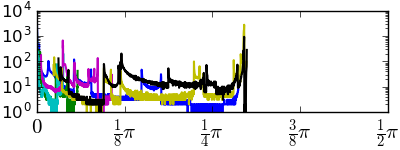
\includegraphics[width=0.45\textwidth]{tangency_ppo147_1}
    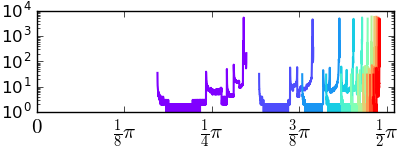
\includegraphics[width=0.45\textwidth]{tangency_ppo147_2}
    \caption{The histogram of angles for \reffig{fig:smallestAngle}. The
    crazy peaks are presumably due to the smooth oscillation of the angle
    along the orbit - every peak or bottom becomes a square-root singular
    cusp in the histogram}
    \label{fig:tangency_ppo147}
  \end{figure}

\item[2016-02-26 Kazz to Xiong]
Thanks.  Could you give me the data so that I can check how they behave near $\theta=0$? I'd like to see how the histogram in the left panel
 look like near $\theta=0$, say in the range $0 \leq \theta \theta 10^{-5}$.

\item[2016-02-26 Kazz to Xiong \& Evangelos]
Thanks Xiong for the data.
I made the histogram of the angle shown in \reffig{fig:smallestAngle},
 in \reffig{fig:histogram1}.
  \begin{figure}
    \centering
    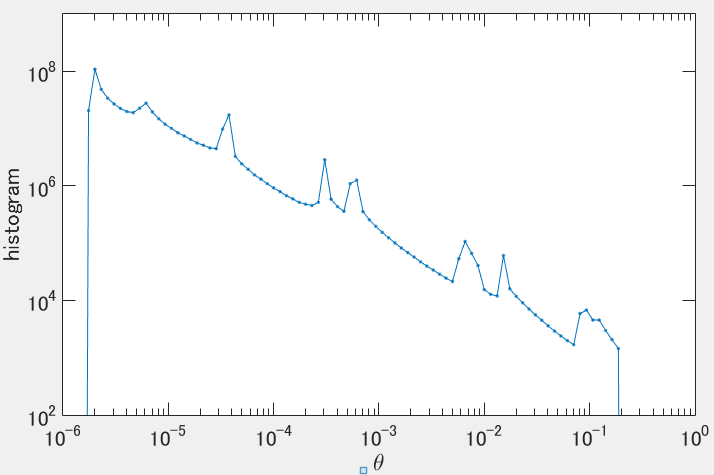
\includegraphics[width=0.6\textwidth]{histogram1}
    \caption{Histogram of the angle shown in \reffig{fig:smallestAngle}}
    \label{fig:histogram1}
  \end{figure}
Although the histogram density takes very large values near $\theta=0$,
it suddenly drops to zero before reaching $\theta=0$, simply because the
minimum angle reached during the finite period of the orbit is strictly
positive, albeit very close to zero. So in this sense, the density
$\rho(\theta)$ always goes to zero as $\theta \to 0$ if $\theta$ is taken
from a single orbit, whereas it can take a non-zero value if $\theta$ is
taken from a collection of (infinitely many) orbits. That's because, as
the number of orbits used in the histogram is increased, the minimum
angle reached by those orbits decreases and can be as small as we want. I
hope this answered Evangelos' question about the angle distribution.

%\reffig{fig:histogram1}

\item[2016-02-29 Evangelos to Kazz and Xiong] Thanks a lot to both for preparing these figures.
I think that \reffig{fig:smallestAngle} illustrates why we cannot use a single orbit.
If I count the number of lines at the left panel correctly, it would lead us to think that
the dimension is $6$ instead of $7$ (but I might miscount here?). I think that in general
you would get a different value for the dimension from different orbits and this is why
you need a collection of them. This is why Kazz's initial attempt long time ago to use
a single orbit gave a result which did not agree with Lyapunov vector predictions.

Regarding \reffig{fig:histogram1}, if the orbit that you use is the one that gives you the minimal
angle, then you would not get any better result if you would plot Fig. 2 of the manuscript
in log-log scale. I don't think that this is alarming since in a numerical computation with
a finite number of steps you can get only to finite distance from zero angle.

For me the manuscript is good to submit but I would prefer the sentence that
says that tangency cannot be reached during a finite period of time to be changed.

\item[Xiong to Evangelos]
Each orbit has 2 marginal directions.
The reason that the left panel of \reffig{fig:tangency_ppo147} has
only 6 lines is that I choose not to set the index $k$ cutting
between these
2 marginal \Fv s. Since the index of marginal directions differs
for different orbits (some orbits have only 1 unstable \Fv, and
others have 2), the plot of the collection of all 400 orbits have 7
lines.

\item[2016-02-29 Kazz to Evangelos and Xiong]
Xiong is right, we do find the same threshold for any single orbit, if it is appropriately determined. The problem of the angle distribution is that we cannot set any threshold in an appropriate way for a single orbit, because strictly the angle for any pair of vectors/subspaces cannot reach zero during the finite period of the orbit. This is also the problem I and Hugues argued five years ago.

Anyway I agree that we need to rephrase some sentences in the manuscript. I'm taking charge of this work (and making a new figure showing the local exponent). After this change, I also believe the manuscript is ready to submit!

\item[2016-02-29 Kazz to Predrag]
I realized some questions asked previously to you remain unanswered:

1. Is the Navier-Stokes equations believed to have a finite-dimensional
inertial manifold?
\\ {\bf 2016-03-01 Predrag}
Be very cautious here - what
Temam\rf{temam90} writes, still applies today:

\begin{quote}
the existence of an inertial manifold is still an open problem. In
particular this is the case for the Navier-Stokes equations
\end{quote}

I have now incorporated this into the manuscript. Do not make any claim
stronger than that. I find the \HREF{http://arxiv.org/pdf/1303.4457.pdf}
{mathematical literature}\rf{Zelik14} mind-boggling impenetrable, so less
we claim about `inertial manifolds' the better.

2. Do you know any important study on the periodic orbit expansion that
does NOT come from your group (and is worth mentioning in our paper)?
\\
{\bf 2016-03-01 Predrag} Yes, I like Wintgen \etal\ work\rf{WRT92} very
much, and can dig up some other references were they needed. But it his
paper we \emph{should not} refer to any `periodic orbit expansions'
\emph{at all}, as we are in no position to apply the theory to kind
of data we have (yes, we have 60\,000 \rpo s, but they were found by
blind night fishing): we have no qualitative partition of the \KS\
attractor, no hint of symbolic dynamics, or any understanding of which
orbits shadow which orbits.

\item[2016-02-29 Kazz to everyone]
Since I get no objection about the use of ``physical'' and ``spurious''
modes, as well as about the abbreviation ppo/rpo, I'm going to bring them
back. Any problem?

\item[2016-03-01 Predrag to Kazz]
It's a big problem, and objections have been loud, for at least two years
already. These terms are macros in

\texttt{siminos/dimension/upodimDefs.tex},

easily flipped back and forth by commenting the lines in the macros, so
do not stick the words into the main text, we can experiment by changing
the macros.

Why `spurious' is not appropriate? You do not use it in the sense the
word is used in English, please reread {\bf 2014-01-26 Predrag} above. I
suggest using `transient' instead, it says what we mean it to say.

For example, Temam\rf{temam90} writes

\begin{quote}
Because the inertial manifold is approached at an exponential rate,
we see that after a certain transient period, the orbits lie on it during
the permanent regime: during the permanent regime small and large
wavelengths phenomena are connected by the quasistatic law (15).
\end{quote}

(By `permanent', `quasistatic' he means steady turbulence)

Inertial manifolds are finite-dimensional, smooth, invariant manifolds
that contain the global attractor and attract all solutions exponentially
quickly. I have not seen source literature that describes their dimension
as `physical', everybody simply says `finite-dimensional'.

There is nothing `physical' about about numerical simulations of an
applied mathematics equation like \KS, no physical about it, and on top
of everything, studied on the embarrassingly small and totally unphysical
$L=22$ domain. Abusing the word just annoys our colleagues for no good
reason - our work is interesting not because it is `physical' but because
it makes the notion of finite-dimensionality of intertial manifolds
tangible and computable. If it works out for Navier-Stokes, that will be
`physical'.

By the way, I have already done what you want to do with by putting
`physical dimension' in quotes in the abstract, writing in the current
draft

\begin{quote}
a finite-dimensional subspace of
``{\entangled} Lyapunov modes'' (referred to in what follows as the
``physical manifold''), which is presumed to carry all dynamically
relevant information, and the remaining infinity of ``{\transient}
Lyapunov modes''.
\end{quote}

and then using `physical' throughout, so there is nothing further in the
manuscript for you to make `physical'.

I really  do not know where this `physical dimension' term comes from...
Can you find it anywhere in source literature on inertial manifolds? Take
Temam\rf{temam90} for example - clearly written and simple.

\item[2016-02-29 Kazz to everyone]
As these words appear many times, it seems to me much easier to
restart from the version Hugues and I prepared, then apply changes made
by now (except physical/spurious and ppo/rpo). Any problem?

\item[2016-03-01 Predrag to Kazz]
{\large Please do not resurrect}
your draft of February 1 - the current draft is your draft, subsequently revised. If
you need the initial text for some reason, it is in rev.~4596, called
\texttt{upodim-2.tex}. All the references have been changed to what they
are called in \texttt{bibtex/siminos.bib} (that is needed so Xiong can merge
contenct of this paper into his PhD thesis), and much of the paper has been
rewritten by Evangelos, Ruslan and me, so just keep working on
DCTSCD14.tex. Trust us, this is your draft of February 1, with subsequent
edits by your collaborators, nothing you wrote has been lost, its been
only improved. And no need to rename it again, svn keeps track of every
single edit ever made to the paper, nothing is ever lost. Wonders of
modernity.

You do not have to wait for others to stop editing. The structure of
current draft is good, we are only doing local edits, not global
reorganizations. The work cycle is this - every so often (could be 15
minutes after you started editing) you commit your edits - then it's
someone else's problem to resolve conflicts, if any :)

\item[2016-03-03 Kazz to Predrag and everyone]
Thanks Predrag for the improvement and the explanations. Myself I am more liberal about the usage of the word "physical", but I'm not strongly for this name either. So I agree to change the names to "entangled" and "transient", provided that I can inform readers by a footnote that the names have been changed from those used in previous publications. About ppo/rpo, I don't insist on using these abbrevations.

Anyway, I finished revising the text, incorporating our recent updates on the local exponents and the angle distribution, and updating figures 1 and 2 accordingly. Now I'd like you all guys to make a final check of the manuscript (and cover letter, 50-word summary).

\item[2016-03-04 Xiong ]
For this version, I have some minor questions.

1. In the abstract, ``we determine the dimension of the inertial manifold
for a Kuramoto-Sivashinsky system''. should we delete 'a' in front of
'Kuramoto-Sivashinsky system' ? \\
{\bf 2016-03-04 Kazz to Predrag}
I'd like Predrag to judge this.

2. At page 6, the definition of local Floquet exponents. The definition
of stability matrix is
$A(x)\equiv\frac{\partial{}J^\tau}{\partial\tau}(x)|_{\tau=0}$,
which is correct, but not how we generate it. Usually, we take
$A(x) = \partial v(x) / \partial x$. Here $v(x)$ is the velocity field
$\dot{x} = v(x)$ of the system. \\
{\bf 2016-03-04 Kazz}
I know; I give it as a definition as you see by the $\equiv$ symbol, and I didn't write that we computed using this definition.

3. About the sentence ``tangency
cannot be reached during a finite period of time by any pair of Floquet subspaces, if one
only looks at a single orbit.'', I understand the subtlety from previous
discussion, but I am
afraid that readers will get confused the first time they read it, as
we did before. \\
{\bf 2016-03-04 Kazz}
See my reply to Evangelos below.

Also, I think we can let the editors and readers to judge these details,
and submit it right away.

\item[2016-03-04 Evangelos to Xiong and Kazz]

Kazz writes: ``Interestingly, the distribution for small $n$ has a strictly
positive density at $\phi\to0$, even though no single orbit can reach strictly vanishing angle.
This implies that the smallest angle reached by a collection of orbits becomes as small as we wish,
as we increase the number of the orbits.''

Sorry that I will keep asking the same question,
but the above statement is thought provoking
and I need to understand it.

If you plot Fig. 2 of the manuscript
in log-log scale, how would it be different than \reffig{fig:histogram1}?
Xiong could you please do that? Don't you have a sharp
cutoff at $10^{-6}$ also at this case?

Also, Xiong do you indeed as Kazz suggested,
always get the same threshold from all individual
orbits from figures like \reffig{fig:tangency_ppo147}?
What happens if you take the shortest orbits?
Say, the shortest PPO?

The reason I ask is this:
if the angle obtained from all orbits is strictly
bounded away from zero
but the minimal value on an orbit
becomes smaller for longer orbits
(which is not unreasonable)
then indeed we would get to the $\theta\rightarrow 0$
limit as longer orbits are added.
However we have not shown that the angle is
bounded away from zero. In numerics how close
we get to zero depends
on the time step size used and one could argue that
using smaller time step we could get smaller angles
from a single orbit, instead of adding more orbits.
So I am afraid to make a general claim like the one
above.
(The situation would be different if the
angle could be defined in such a way that it changes
sign as it goes through zero.)

The other possibility is that I totally miss the point
that Kazz is trying to make...

\item[2016-03-04 Kazz to Evangelos and Xiong]

Okay, I did some exercise to convince you.

Let's consider a very simple situation, inspired by the observation in \reffig{fig:histogram1}: I assume that the angle distribution of a single orbit is
\begin{equation}
\rho_\textbf{single}(\phi; \phi_0) =
\begin{cases} 0 & (\phi < \phi_0) \\ c/\phi & (\phi > \phi_0) \end{cases}
\end{equation}
with an orbit-dependent, strictly positive parameter $\phi_0$ and a positive constant $c$ (that may depend on $\phi_0$).
Now every orbit has a different value of $\phi_0$, so its distribution is given by a function, say, $\rho_\textbf{orbit}(\phi_0)$.
Therefore, the angle distribution for the collection of orbits is given by
\begin{equation}
\rho_\textbf{collection}(\phi) = \int \rho_\textbf{single}(\phi; \phi_0) \rho_\textbf{orbit}(\phi_0) d\phi_0.
\end{equation}

Now I assume $\rho_\textbf{orbit}(\phi_0) \to \rho_0 > 0$.
Then, for small $\phi$, we can show
\begin{align}
\rho_\textbf{collection}(\phi)
 &= \int \rho_\textbf{single}(\phi; \phi_0) \rho_\textbf{orbit}(\phi_0) d\phi_0 \notag \\
 &= \int_0^\phi (c/\phi) \rho_\textbf{orbit}(\phi_0) d\phi_0 \notag \\
 &\simeq (c/\phi) \rho_0 \phi = c\rho_0 > 0
\end{align}
So $\lim_{\phi \to 0} \rho_\textbf{collection}(\phi)>0$ even though
$\lim_{\phi\to 0}\rho_\textbf{single}(\phi; \phi_0) = 0$ for \textit{any} orbit.
However I think this argument is too tedious and speculative to include in the manuscript. To me it seemed clear that the statement I made was possible, at least in principle, so I was not expecting it was so difficult to have this accepted (well I'm not sure if I succeeded..).


\item[2016-03-04 Xiong]
I thought I understand the subtleties before, but now I can
hardly get the point of the discussion.
My understanding is very simple, which is rooted in
the sentence ``bounded away from zero''. For me, it means,
we can find a fixed $\phi_c > 0$, such that
$\rho(\phi \le \phi_c) = 0$. This corresponds to a threshold in
Fig.2. Hyperbolicity indicates that
such a positive number does not exist. No matter
how small a number you choose, the density can go beyond this number
by studying more orbits. However, numerically it is impossible to test
this number goes infinitely close to zero with only a finite set of
orbits, so when it is extremely
small then it is fine. But who knows how to judge whether it is
extremely small or not, so the contrast plays the role. One set
reaches a really small angle $10^{-6}$,
the other set stop at $\pi/10$. By studying only
one orbit, for example, the two numbers may be $10^{-2}$ and $\pi/10$,
the contrast may not be manifest.
\refFig{fig:tangency_ppo147} has good contrast but it is picked
intentionally.

\item[2016-03-04 Kazz to Xiong]

So you didn't understand my argument, right? But as you didn't mention anything about my argument, I don't know where you don't get it. Could you specify it?

About what you wrote, of course numerically we cannot go to absolute zero, so we extrapolate. If we do so, Fig.2 shows that $\rho(\phi) > 0$ at $\phi \to 0$,
 non? If you want to be more careful, just change the number of orbits you use, and see how the minimum angle descreases as a function of the number of orbits.


\item[2016-03-04 Xiong to Predrag]
I think the local \Fe s are not invariant under coordinate transform.
\[
  \lambda_i(x) = \frac{e_i^\dagger(A^\dagger+A)e_i}{2e_i^\dagger e_i}
\]
Here, the denominator is a normalization factor. For a state
transform $y=h(x)$, the velocity changes as $\dot{y} = h'(x)\dot{x}$,
so $v'(y) = h'(x) v(x)$. Therefore,
\[
  A'(y) = \frac{\partial v'(y)}{\partial y}
  = \frac{\partial (h'(x)v(x))}{\partial v(x) }
   \frac{\partial v(x)}{\partial x }\frac{\partial x}{\partial y}
  = h'(x) A(x) \frac{1}{h'(x)}
\]
Also \Fv s are transformed as $e'_i(y) = h'(x)e_i(x)$, so
\[
  \lambda'_i(y) = \frac{e_i^\dagger(A^\dagger h'^\dagger h' +
    h'^\dagger h'  A)e_i}
  {2e_i^\dagger h'^\dagger h' e_i}
\]
Factor $ h'^\dagger h'$ appears. Does it make sense ? My
understanding is that coordinate transform is somewhat
equivalent to using different norms in this case.  Then a vector
rotated to another orientation will have different
norm. You said infinitesimal expansion/contraction will get stretched by
this transform and the original vector gets stretched too, so the
ratio should not change. But I think the measurement depends on
the orientation of the stretched vector.
 \\
{\bf 2016-03-07 Predrag} Your argument looks correct to me, and
\refref{BosPos14} also says that the local Lyapunov is not coordinate
invariant. It would be a bit of a miracle...

\item[2014-11-19, 2016-03-04 Predrag]
In continuum mechanics / soft cond. matter physics
one visualizes {\stabmat} / {\velgradmat} $\Mvar$
as the rate of deformation, and decomposes it into the antisymmetric
and symmetric parts, $\Mvar = \Omega + D$. Then the Lyapunov equation
\beq
\dot{\covMat} = \Mvar \covMat + \covMat \transp{\Mvar} + \diffTen
    \,,\qquad
\covMat(t_0) = \covMat_0
\,.
\ee{contLyapODE}
takes form
\beq
\dot{\covMat} = [\Omega, \covMat]
                \pm (D \covMat + \covMat D)
                 + \diffTen
\,.
\ee{contLyapRot}
$\Omega$ generates rotations. The eigenvalues and eigenvectors of
the symmetric matrix $D$ are understood in
\HREF{http://www.streamsound.dk/book1/chaos/chaos.html\#133/z} {polar
decomposition} as principal stretches. The $\pm$ in \refeq{contLyapRot}
is way of pulling out explicitly the signs of principal stretches, and
thus keeping track of whether the deformation is `prolate' and `oblate'.
They maybe also have to look into the mixed signs (our hyperbolic case)
and worry about marginal signs and degenerate eigenvalues, might be
useful to check some of that literature.
They find it useful to
(\HREF{https://en.wikipedia.org/wiki/Strain_rate_tensor}
{following} Landau and Lifshitz\rf{Landau59a})
separate $D$ into its trace (isotropic part) and the traceless part
(non-isotropic deviation):

Any matrix can be decomposed into the sum of a {\em symmetric matrix} and
an {\em antisymmetric matrix}.
Applying this to the \stabmat\
\(\Mvar = (\nabla v)^T\) with symmetric and antisymmetric components
\(D\) and
\(\Omega\) respectively:
\[
  D = \frac{1}{2}\left( \Mvar + \Mvar^\mathsf{T}\right)\quad\quad\quad
  \Omega = \frac{1}{2}\left( \Mvar - \Mvar^\mathsf{T}\right)
\]
That is,
\[
  D_{i j} = \frac{1}{2}( \partial_j v_i + \partial_i v_j ) \quad\quad\quad
  \Omega_{i j} = \frac{1}{2}( \partial_j v_i - \partial_i v_j)
\]
This decomposition is independent of coordinate system, and so has
physical significance. Then the velocity field may be approximated as
\(v(\ssp + \deltaX,t)
\approx v(\ssp,t) + D(\ssp,t)\deltaX + \Omega(\ssp,t)\deltaX,\) that is,
\[
  \begin{array}{lcl}
    v_i(\ssp + \deltaX,t) &=&
      v_i(\ssp,t) + \sum_j D_{i j}(\ssp,t) \deltaX_j + \sum_j \Omega_{i j}(\ssp,t) \deltaX_j\\
    ~ &=&
      v_i(p,t)
      + \frac{1}{2}\sum_j \left(\partial_j v_i(\ssp,t)+\partial_i v_j(\ssp,t)\right)\deltaX_j
      + \frac{1}{2}\sum_j \left(\partial_j v_i(\ssp,t)-\partial_i v_j(\ssp,t)\right)\deltaX_j
  \end{array}
\]
In 3 dimensions (not relevant here) the antisymmetric term
\(\Omega\) represents a rigid-like rotation of the \statesp\ element about the point
\(p\).  Its angular velocity
\(\omega\) is
\[\omega=\frac12 \nabla\times v=
\frac{1}{2}
\begin{bmatrix}
\partial_2 v_3-\partial_3 v_2\\
\partial_3 v_1-\partial_1 v_3\\
\partial_1 v_2-\partial_2 v_1
\end{bmatrix}.
\]
The product \(\nabla\times v\) is called the ``{\em rotational}''
``curl'' of the vector field.   A rigid rotation does not change the
relative positions of the \statesp\ elements, so the antisymmetric term \(\Omega\)
of the velocity gradient does not contribute to the rate of change of the
deformation.  The actual strain rate is therefore described by the
symmetric \(D\) term, which is the ``{\em strain rate tensor}''.

The symmetric term \(D\) of velocity gradient (the rate-of-strain tensor)
can be broken down further as the sum of a scalar times the {\em
Kronecker delta}, that represents a gradual isotropic expansion or
contraction; and a {\em traceless} symmetric tensor which represents a
gradual shearing deformation, with no change in volume\rf{Landau59a}:
\(D(\ssp,t) = \hat{D}(\ssp,t) + S(\ssp,t).\) That is,
\[
D_{ij} =
\underbrace{\frac{1}{d}(\sum_k\partial_k v_k)
\delta_{ij}}_{\text{rate-of-expansion tensor} D_{ij}}
+
\underbrace{\left(\frac{1}{2}\left(\partial_i v_j+\partial_j v_i\right)
-\frac{1}{d}(\sum_k\partial_k v_k) \delta_{ij}\right)}_{\text{rate-of-shear tensor} S_{ij}},
\]
Here
\(\delta\) is the unit tensor, such that
\(\delta_{ij}\) is 1 if \(i = j\) and 0 if \(i \neq j\).
This decomposition is independent of the choice of coordinate system, and
is therefore physically significant.

The expansion rate tensor is $1/d$ of the {\em divergence} of the
velocity field:
\[ \nabla \cdot v = \partial_1 v_1 + \partial_2 v_2
  + \cdots + \partial_d v_d;\]
which is the rate at which the volume of a fixed amount of \statesp\
increases at that point.

The shear rate tensor is represented by a symmetric $[d\times d]$ matrix,
and describes a flow that combines compression and expansion flows along
three orthogonal axes, such that there is no change in volume.  This type
of flow occurs, for example, when a {\em rubber} strip is stretched by
pulling at the ends, or when {\em honey} falls from a spoon as a smooth
unbroken stream.

============ back to noise - will edit later ================

We think of the `damping term' $\diffTen(\ssp)$ as the noise covariance
matrix (energy is put into the system by the deformation $\Mvar$). For
them it is typically
\beq
\diffTen = - \lambda \frac{\delta F}{\delta \covMat}
\,,
\ee{eq:Olmsted1}
where functional $F[ \covMat]$ is constructed
from invariants one can get out of the matrix
$ \covMat$; $\tr ( \covMat^2)$,
$\tr ( \covMat^4)$ and so on.

Peter Olmsted wants us to read his \refref{Olmsted94}, in particular the Appendix.
His intuition is all $3D$, so it is full of curls and cross products, but
it should makes sense for \statesp\ flows in arbitrary dimension.

\item[2016-03-06 Predrag, from ChaosBook]
Consider the $i$th Floquet multiplier, eigen\-vector pair
$(\ExpaEig_{j},\, \jEigvec[j])$ computed from $\jMps_p$
evaluated at a periodic point $\ssp$,
\beq
\jMps_p (\ssp) \,\jEigvec[j](\ssp) =
    \ExpaEig_{j} \,\jEigvec[j](\ssp)\,,  \quad
\ssp \in \pS_p \,.
\ee{e-transp}
%and at
Consider another point on the cycle at time $t$ later,
$\ssp'=f^t(\ssp)$ whose \FloquetM\ is $\jMps_{p} (\ssp')$.  As
$\jMps^{\period{}+t} = \jMps^{t+\period{}}$,
the \jacobianM\ at $\ssp'$ can be written either as
\index{semigroup!dynamical}
\[
\jMps^{\period{}+t} (\ssp) = \jMps^{\period{}} (\ssp') \, \jMps^{t} (\ssp)
               = \jMps_p (\ssp') \, \jMps^t (\ssp)
\,,
\]
or
$ % \jMps_p (\ssp') \, \jMps^t (\ssp) =
  \jMps^t (\ssp) \, \jMps_p (\ssp)$.
Multiplying \refeq{e-transp} by $\jMps^t (\ssp)$, we find that the
\FloquetM\ evaluated at $\ssp'$ has the same Floquet multiplier,
\beq
\jMps_p (\ssp') \,\jEigvec[j](\ssp') =
    \ExpaEig_{j} \,\jEigvec[j](\ssp')\,,  \quad
     \jEigvec[j] (\ssp') = \jMps^t (\ssp) \,\jEigvec[j](\ssp)
\,,
\ee{EigsInvar}
but with the eigen\-vector $\jEigvec[j]$ transported along the flow
$\ssp \to \ssp'$ to $\jEigvec[j](\ssp')=\jMps^t(\ssp)
\,\jEigvec[j](\ssp)$. For infinitesimal time, $\jMps^{dt}(\ssp)
= (1+ dt\Mvar(\ssp))$, so the change of the eigenvector is
\beq
\frac{d~}{dt} \jEigvec[j](\ssp) = \Mvar(\ssp)\,\jEigvec[j](\ssp)
= (\Omega + D)\,\jEigvec[j](\ssp)
\,.
\ee{FloqVecEvolution}
We already know this equation, as $\jEigvec[j](\ssp)$ is a column of the
Jacobian $\jMps^t(\ssp)$. The rotation  and deformation rates $\Omega$,
$D$ (defined in \refeq{contLyapRot}) cannot be integrated separately, as
$\Mvar$ is non-normal, $[\Mvar,\transp{\Mvar}] \neq 0$.

While the rotation and deformation rates do not commute, Xiong still
might be able to use this decomposition in his Schur integrations, by
splitting the Jacobian into infinitesimal steps (also from ChaosBook) and
keeping terms up to $\timeStep^2$ in
\beq
\jMps^\timeStep=\hat{\jMps}^\timeStep
+{1 \over 24} \timeStep^3 [\Omega +2D ,[\Omega ,D ]] + \cdots
\,,
\ee{3.43ab}
where
\beq
\hat{\jMps}^\timeStep =
e^{\half \timeStep \Omega }
e^{\timeStep D }
e^{\half \timeStep \Omega }
\,.
\ee{split_prop}
The approximate infinitesimal Jacobian
$\hat{\jMps}^\timeStep$ is now a sequence of mappings,
a rotation by $\half \timeStep \Omega $, deformation by
$ \timeStep D $,
followed again by $\half \timeStep \Omega $ rotation.
As we already have the orbit
\[
\ssp_p(t) = \ssp(\ssp_0,t) \,,\qquad \ssp_0 \in p
\,,
\]
integrating this Floquet eigenvector (rather than the Jacobian matrix)
might work out in the {\psd} setting. For rotations, there might be a natural
basis to express the antisymmetric matrices in,
\[
\Omega = \sum_\alpha^N \theta_\alpha \Lg_\alpha
\,,\qquad N = d(d-1)/2
\,.
\]
The simplest is a matrix with only two $\pm 1$ entries,
\[
(\Lg_\alpha)_{ij} = 1, (\Lg_\alpha)_{ji} = -1 \mbox{ for a given } i<j
\,,
\mbox{ zero elsewhere}
\,,
\]
but that looks stupid as it does not rotate leading
Floquet vectors first.

Assuming a norm, the change in the length of the eigenvector
(dilation) is given by
\[
\frac{d~}{dt} \transp{\jEigvec[j](\ssp)}\cdot\jEigvec[j](\ssp)
=  \transp{\jEigvec[j](\ssp)} (\transp{\Mvar(\ssp)} + \Mvar(\ssp)) \jEigvec[j](\ssp)
\]
so the symmetric matrix $ 2 D(\ssp) = \transp{\Mvar(\ssp)} + \Mvar(\ssp)$
is the rate of deformation (change of the length of the eigenvector),
while the antisymmetric part $ 2 \Omega(\ssp) = \transp{\Mvar(\ssp)} - \Mvar(\ssp)$
is its rotation velocity. Mimicking \refref{BosPos14} definition of
the local Floquet exponent as
\beq
\lambda_{j}^\textrm{loc}(\ssp) \equiv \lim_{\tau\rightarrow 0}\lambda_j^\tau(\ssp)
= \transp{\jEigvec[j](\ssp)} \Mvar(\ssp) \jEigvec[j](\ssp)
\,,
\ee{BosPos14}
is wrong, it should be
\beq
\lambda_{j}(\ssp)=  \transp{\jEigvec[j](\ssp)}
\frac{\transp{\Mvar(\ssp)} + \Mvar(\ssp)}{2} \jEigvec[j](\ssp)
\,.
\ee{PC16}
Notation $\lambda_{j}^\textrm{loc}(\ssp)$ is superfluous, it suffices to
indicate `local' by $\lambda_{j}(\ssp)$, and the (true), coordinate independent
 Floquet exponent by  $\lambda_{j}$. $\lambda_{j}$ is not a simple
average of $\lambda_{j}(\ssp)$ over the periodic orbit, as the Floquet eigenvector is
also rotated by the (antisymmetric) rotation generator $\Omega(\ssp)$.


\item[2016-03-02 KT] The Floquet exponents are by definition real
numbers, even for complex Floquet multipliers.

\PCpost{2016-03-04}{
Wow, I did not know that. Can you give me the reference that explains
this fact about \emph{Floquet} (not Lyapunov) exponents, \ie, that a
logarithm of a complex number is real? I better correct that in
ChaosBook. Also Burak's paper\rf{Bud15} (\texttt{pipes/torsion/}
repository) will have to rewritten.

Kidding aside, check, for example Eq.~(3.29) in these
\HREF{http://www.emba.uvm.edu/~jxyang/teaching/Floquet_theory_Ward.pdf}
{lecture notes}.
    }

    \PCpost{2016-03-05}{
Out of curiosity (where does Kazz belief that Floquet exponents are ``by
definition'' real come from?) I learned something I did not know:
Montagnier, Paige and Spiteri\rf{MoPaSp03}
{\em Real {Floquet} factors of linear time-periodic systems} write:
``It is well known that it is always possible to obtain a real Floquet
factorization for the fundamental matrix of a real T-periodic system.''
This ``factorization''\ie, the Floquet exponent matrix (logarithm for the
Floquet matrix) can always be chosen real. It's eigenvalues, or `Floquet
exponents' are either real or come in complex pairs, as usual.
The paper is worth a read.

Basically, Lyapunov's reducibility theorem states that there exists a
\emph{Lyapunov–Floquet transformation} of the original coordinates
$\ssp(\zeit)$ that renders the \stabmat\ od the periodic system
\[
\dot{\ssp}(\zeit) = {\Mvar}(\zeit)\ssp(\zeit)
\]
time-invariant,
\beq
\dot{\ssp}(\zeit) = {\Mvar}_L \ssp(\zeit)
\,.
\ee{constA}
There is endless literature on this\rf{JosSat72}.
There is even something specifically written for Burak in my favorite
periodical, {\em Journal of the American Helicopter Society}. Peters,
Lieb and Ahaus\rf{PeLiAh11} {\em Interpretation
of {Floquet} eigenvalues and eigenvectors for periodic systems}, write:
``The application of Floquet analysis to rotorcraft has demonstrated that
there is often misunderstanding as to how to interpret the
integer-multiple arbitrariness in the imaginary part of the
characteristic exponents of the system (i. e., in the frequency).
Although some papers have offered various methodologies for choosing the
{\em correct} frequency (such as choice of the strongest harmonic in the
periodic eigenvector), confusion still persist and none of the proposed
methods completely solves the difficulty. The purpose of this present
paper is to (1) offer a history of analysis of periodic systems with
respect to the treatment of the integer multiples, (2) propose a
practical tool for fundamental insight into system frequencies, and (3)
show demonstratively for simple cases why no single integer can
adequately describe system dynamics. It is hoped that this approach will
provide clarity to a problem that, although long understood in principle,
still leads to confusion in published papers.''

Regardless of whether we like this paper, it cites some papers which
we might have to also cite in \refref{Bud15}.
}

\item[2016-03-06 Xiong]
\refref{MoPaSp03} does not say that Floquet exponents should be real
\PCedit{(Predrag: of course not)}.
Floquet theory only says that for a solution
with period $T_p$, the Jacobian or monodromy matrix can be written as
$J^t(x) = e^{t B}$
\PCedit{(Predrag: there is a bit more to it - this can be factored in
such a way that the matrix in the exponent can be made into a constant
matrix ${\Mvar}_L$, as in \refeq{constA})}.
Matrix $B$ has period $T_p$ and could be real or complex with its
eigenvalues the Floquet exponents. If $B$ is complex, then we can find a
real matrix $R$ such that $J_t(x) = e^{t R}$. $R$ has period $2T_p$. It
does not mean that the eigenvalues of $R$ should be real.

But local Lyapunov exponents are always real. The definition of local
Floquet exponents mimics the definition of local Lyapunov exponents, so
we need to take symmetric part to make the definition work for both real
and complex cases. See [2016-02-15 Xiong].
\PCedit{(Predrag: no problem there - you have the correct definition in
the complex case, but for some reason drop $\Re$ on the LHS of
\(
\Re\lambda_{j}(\ssp)= \Re\left[
\transp{\jEigvec[j](\ssp)}\Mvar(\ssp)\jEigvec[j](\ssp)
                          \right]
%\,.
\)
    )}

    \PCpost{2016-03-06}{
Xiong writes: ``The definition of local Floquet exponents mimics the
definition of local Lyapunov exponents.'' But why \emph{we} should it?
Who has defined ``local Floquet exponents'' other than us? There are lots
of people who run long trajectories and only look numerically at the rate
with which a distance (in a given norm) along a given \cLv\ changes on
average, but why should we lim it us to that? They have no way of making
sense of rotation rates, but that is not our problem. Dynamical systems
theory gives us the tools to piece together the full geometry of the
\nws\ by finding invariant solutions (invariant local, linearized
description of each neighborhood: its dilatations and rotations) and the
invariant heteroclinic connections between them (how these neighborhoods
hang together globally). That is what \emph{we} bring to the `physical
dimensions' community, they can run their large simulations perfectly
well without us (and much more efficiently than us).

The rotation rates of spiral-in or spiral-out Floquet eigenplanes are
essential if one is to piece together global dynamics, organize
infinities of \po s and construct symbolic dynamics. This discussion goes
back to Xiong's claim that it is not possible to assign a rotation rate
(phase per unit time) to a complex Floquet pair of modes. Is Burak's
paper wrong\rf{Bud15}?

And why object to this wording:

\begin{quote}
The Floquet exponents $\lambda_j$
(if complex, we shall only consider their real parts, with multiplicity 2)
are related to multipliers by $\lambda_j=\ln|\Lambda_j|/\period{p}$.
\end{quote}

? It answers the obvious question which a dynamical systems reader would
have (they all know that Floquet exponents are complex), and then we move
on - we do it in \refref{DCTSCD14} because \cLv\ people (those who call
everything that Lyapunov did not do `Lyapunov' :) can only compute the
real parts, so there is nothing else to compare to. Obviously
neighborhoods of chaotic trajectories rotate as well, but they do not
know what to do with that, because they have no controllable way
describing recurrences, other than measuring distances in an arbitrary
norm. Not our problem.
    }

    \PCpost{2016-03-06}{
Talking about `arbitrary norms': can we argue that for \KS\ the L2 norm
is The Norm because of the \On{2} equivariance? It leads to the Fourier
modes basis (IF one ignores the fact that this is a highly non-linear
problem, and throws out the baby with the water by dropping the nonlinear
terms) and to near orthogonality of the high modes. Of course, in fluid
dynamics the enstrophy norm (square the curl of $u_j(x,t)$) is equally
good, as are other Sobolev norms, so I do not know how far we can get
with that argument.
    }

\item[2016-03-07 Burak] I had been reading the blog and thinking
about this subject over the weekend. For now, I would just like to
summarize my understanding. First and foremost, complex phase of a
Floquet multiplier does not correspond to a "polar angle": It is the
parameter in a particular parametrization of an ellipse. Let
$(\ExpaEig_{j},\, \jEigvec[j])$ be a complex Floquet multiplier/vector
pair computed at a periodic point $\ssp$. Let us consider the linear
discrete time dynamics of a small perturbation
$\delta \ssp = \epsilon \Re \jEigvec[j]$ to $\ssp$ at times
$n \period{}$
\beq
    \delta \ssp [n] = \epsilon |R|^n
    \left[\cos (n \Omega) \Re \jEigvec[j]
         + \sin (n \Omega) \Im \jEigvec[j] \right] \,,
         \mbox{where } \ExpaEig_{j} = R e^{i \Omega} \, .
    \label{e-DiscreteDynamics}
\eeq
If we forget the expansion/contraction for the moment, generic
linearized trajectories lie on the ellipse
\beq
    \Re \jEigvec[j] \cos \alpha
         + \Im \jEigvec[j] \sin \alpha  \, ,
\label{e-FloquetEllipse}
\eeq
where $\alpha$ is a certain parametrization of an ellipse, which would
only correspond to a polar angle if $\Re \jEigvec[j]$ and
$\Im \jEigvec[j]$ were orthogonal hence ellipse was a circle.
\refeq{e-FloquetEllipse} is also different from the principal axis
parametrization
\beq
    p_1 \cos t  + p_2 \sin t
    \label{e-pAxesEllipse}
\eeq
of an ellipse, where $p_1$ and $p_2$ are orthogonal vectors of different
norm (principal axes) of the ellipse because
$\Re \jEigvec[j]$ and $\Im \jEigvec[j]$ do not coincide with the
principal axes.

Moreover, the parametrization \refeq{e-FloquetEllipse} is not unique
for a small neighborhood since $\jEigvec[j]$ is not, \ie\
$\Re e^{i \theta} \jEigvec[j] \cos \beta + \Im e^{i \theta} \jEigvec[j]
\sin \beta$, where $\theta$ is a finite angle and $\beta$ is the new
parameter, defines the same ellipse with \refeq{e-FloquetEllipse} and
\refeq{e-pAxesEllipse}. However, if we use the principal axes to define
the elliptic neighborhoods as in \refeq{e-pAxesEllipse}, we have only
$4$ possible ways of doing that. Moreover, if we make a particular
choice $p_1, p_2$ for a certain point on a periodic orbit and then
smoothly continue these axes along the orbit, then we obtain an
intrinsic reference frame on which we can measure rotational parts of
the dynamics with respect to principal axes.

I am pretty much convinced that these small changes from one point to
the infinitesimally separated next one on a periodic orbit are not
invariant under coordinate changes, but my intuition is the total
half-integer (for a subtle reason) number of rotations in the tubular
neighborhood with elliptic cross-sections after one return should not
change under coordinate transformations.

In general, I think it is unnatural to separate the dynamics to
symmetric and antisymmetric parts in these neighborhoods as the
non-orthogonality of the real and imaginary parts of the complex
eigenvectors have fundamental implications. For instance, when a
perturbation is evolving according to \refeq{e-DiscreteDynamics} and
$R > 1$, $|\delta \ssp [1]|$ can be smaller than $|\delta \ssp [0] |$
if \refeq{e-FloquetEllipse} happens to define a very stretched
ellipse (the case when $\Re \jEigvec[j]$ and $\Im \jEigvec[j]$ are
almost parallel) and $|\delta \ssp [1]|$ lands on the shorter side
of the expanded ellipse.

Most probably, I am going to rewrite \refref{Bud15} as a way of
characterizing dynamics within neighborhoods of periodic orbits, which
can find applications in control. I have only skimmed the helicopter
paper yet but it might be in similar context because there are many
engineering applications where one wants to stabilize a periodic
motion.

    \PCpost{2016-03-07}{
Xiong did not know what the sentence

\begin{quote}
``a finite-dimensional inertial manifold
on which the dynamics of a chaotic dissipative dynamical system lives can
be constructed solely from the knowledge of a set of unstable
periodic orbits''
\end{quote}

in the abstract of \refref{DCTSCD14} means, so let's recapitualate what
this paper is about, and check whether we actually say the salient parts
in the paper (the overall program has too many moving parts to enumerate
in this PRL):

This is a paper about dynamical theory of turbulence
\begin{enumerate}
  \item
`Geometry of turbulence' (`chaos, `spatio-temporal chaos'):
A strange attractor is organized by a hierarchical set of compact,
time-invariant solutions
(see \refsect{sect:intro}). The key notions:
    \begin{enumerate}
      \item Inertial manifold: a finite-dimensional smooth manifold that
      contains the attracting set, such that all transient trajectories fall into
      it at exponential rate
      \item Recurrence (`shadowing'): a neighborhood of a point (`state')
      is revisited by a generic trajectory. Requires identification of
      physically distinct states (symmetry reduction, symmetry
      quotienting).
      \item `Strange attractor', `\nws': a set of points visited
      arbitrarily closely by a generic ergodic (`chaotic') trajectory. A
      (fractal dimension) set contained within the inertial manifold.
      \item `Periodic orbit theory':
      A tiling of the strange attractor (`generating partition',
      `symbolic dynamics', `Markov graph') by a hierarchical set of
      compact recurrent solutions (`\po s') and their linearized
      neighborhoods. A local `tile' has the dimensionality of the
      \statesp\ minus the number of continuous symmetries (one of which
      is time).
    \end{enumerate}
  \item
  {\Entangled}-{\transient} splitting: \cLvs\ linearization of an
  infinite-time ergodic trajectory (whose computation was made possible
  by the algorithm of \refref{ginelli-2007-99}) defines a local,
  covariantly moving {\entangled} (`physical') hyperplane, and
  establishes that it locally behaves as `inertial manifold': long-time
  dynamics is confined to a fixed dimension finite-dimensional
  hyperplane, with all other eigen-directions falling into it at
  exponential rate (not slower!). Strictly local to an ergodic trajectory
  - no recurrences, and no notion of geometrical embedding into the
  \statesp\ of the system.
  \item
  Ergodic trajectories + recurrences = local notion of geometry:
  \refRef{YaRa11} establishes that a vector separating a pair of
  recurrent points lies in the local physical manifold (is that the paper
  does? Does \refref{TaCh11} exist and do it better?)
  \item This paper establishes that (in the symmetry-reduced \statesp)
    \begin{enumerate}
      \item Each recurrent, `\po s' embedded in the strange attractor
      owns a finite-dimensional tile (a `brick') of the \emph{same}
      dimension (whose computation was made possible by the algorithm of
      \refref{DingCvit14}). This is not obvious: in general, different
      `\po s' are distant from each other, so this dimension did not need
      to be the same.
      \item The \cLvs\ dimension and the Floquet vectors dimension are the same
      \item An ergodic trajectory visits a `\po s' neighborhood within its
      brick: the Floquet vectors and the  \cLvs-defined local
      physical manifolds coincide
      \item We have sufficiently many `\po s' to tile the strange attractor
      by their bricks
      \item (Future - Budanur, Xiong theses) we still lack the `Markov
      graph' (heteroclinic connections) that tells us how to cover the
      attractor by our bricks (a Voronoi cell per periodic point), glue
      them, cover the curvilinear inertial manifold with them, and
      replace the PDE by a physical-dimension set of ODEs.
    \end{enumerate}
\end{enumerate}
Please edit, rewrite freely any part of this outline - if you can make it
shorter and more precise, great!
    }

\item[2016-03-08 Kazz to Predrag, Xiong, and everyone]
Concerning the definition of the local Floquet exponents, look at OUR
definition in the paper: $\lambda_j=\ln|\Lambda_j|/\period{p}$. It is NOT
the log of a complex number, but that of the MODULUS of a complex number,
so why isn't it a real number?
\\
\PCedit{(Predrag: I was just kidding. Floquet\rf{Floquet1883} exponents
have been `exponents' and have been complex since 1883 - nothing we can do
about that fact. I'm use your definition but prefacing it with word `real
part' so we do not look ignorant when an applied mathematician or control
theorist reads this.)}
\\
I'm not saying that this is the only
possible definition of the local exponents, but for our purpose it is a
useful, clearer (at least for comparing with Lyapunov exponents), and
sufficient way to define it.

About whether we need $\Re$ for the following expression or not, in
general what Xiong wrote was correct, but again for our purpose the
matrix $A$ is real, so we don't need the $\Re$ operation:
$\Re\lambda_{j}(\ssp)= \Re\left[
\transp{\jEigvec[j](\ssp)}\Mvar(\ssp)\jEigvec[j](\ssp)
                          \right]$.
\\
\PCedit{(Predrag: $\Mvar$ is real, but eigenvectors may be complex.
Do not worry about, it's just a detail on our manuscript.)}
\\
Please try to understand my claims, which were made on the basis of what
I wrote in the manuscript, before taking them as general claims and
criticizing as such.

Concerning the content of the paper, I agree about what Predrag wrote, but to me the current abstract is a concise (and a bit PRL style) summary of it. I'd like to know which part of it Xiong did not understand.

    \PCpost{2016-03-08}{
Xiong does not understand the words ``can be constructed''
    }

    \PCpost{2016-03-08}{
What really gives me ulcers

\begin{enumerate}
  \item
\CLv s literature uses `local' in two distinct senses. Most of the time
it is local in \statesp, as in linearizing the flow. However, for `local'
Lyapunov exponents they mean `local' in time, \ie, instantaneous. As we
have a perfectly sensible continuum mechanics term `strain rate tensor'
or `rate of deformation tensor'
since mid-19 century, this is really unnecessary. But for this letter,
we'll live with it.
   \item
I would prefer angles to be positive or negative, as the do in
$\transp{x}\cdot y = |x|\,|y|\,\cos \theta$, rather than keeping only the
positive part, as we do. Our plots would look nicer (it is something that
\cLvs\ probably cannot do).
   \item
\refFig{fig:smallestAngle}:
 What is the oscillation of period $\period{p}/8 = 90.15/8 = 11.3$
 superimposed on the the period $90.15$? Do you have a symmetry-reduced
 \statesp\ picture of this \po? Is the leading Floquet eigenvector real
 or complex? If complex, is this its period?
 (Is my rewrite of the figure caption correct?)
   \item
 to be continued
\end{enumerate}
    }


\item[2016-03-10 Xiong to Predrag]
On page 4 of the newest version of dimension draft, should we
move ``We integrate the system (1) numerically, by a pseudo-spectral
truncation .... no guarantee that all orbits up to a given period
have been found'' to the end of the second paragraph on the same
page, because we have not defined ppo and rpo in the first paragraph.

% Also, we introduce strain rate tensor $D(x)$, should we give a
% reference here ?

% I will think about your suggestion of distinguish positive and
% negative angles.


\item[2016-03-14 Xiong to Predrag]
\refFig{fig:ppo147proj}\,(right panel)shows the symmetry reduced
orbit of 147th ppo projected to Fourier modes. The dots
are the locations of peaks in \reffig{fig:smallestAngle}.
there is no obvious distinction of these points compared with
their adjacent ones. Right panel shows angles along the 150th
ppo. There is no such oscillation superimposed on it.

  \begin{figure}[h]
    \centering
    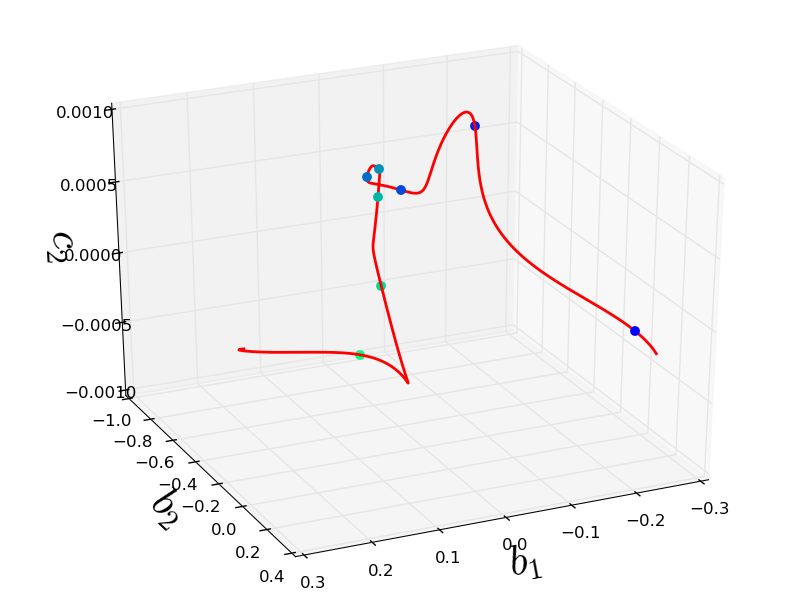
\includegraphics[width=0.48\textwidth]{ppo147unreduced}
    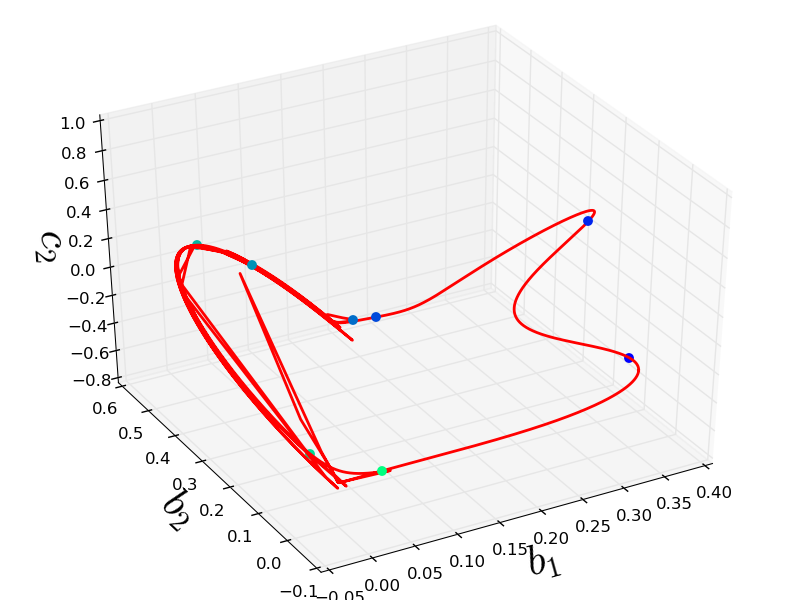
\includegraphics[width=0.48\textwidth]{ppo147reduced}
    \caption{
The $k=1,2$ Fourier components of the 147th \ppo\
(left) In the full \statesp. Note the minuscule $c_2$ component.
(right) In the slice. The $c_2$ component seems larger, but that is
probably an artifact of the {\fFslice}, as are various discotinuities -
big time step glithches.
The peak points (but not the low points) of \reffig{fig:smallestAngle}
are marked on this projection. Hard to know how $k=7$ oscillation
influences the amplitude of $k=1$ and $k=2$ modes, if at all.
    }
    \label{fig:ppo147proj}
  \end{figure}

  \begin{figure}[h]
    \centering
    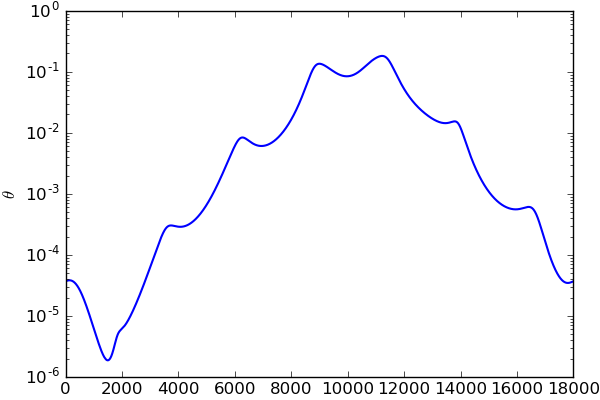
\includegraphics[width=0.6\textwidth]{smallestAngle}
    \caption{
    The principal angle for $k=1$ along the 147th \ppo,
    $\cycle{ppo}_{90.15}$, for one period (horizontal ticks: the number
    of computational integration steps $\Delta{}t\approx0.001$).
    \refFig{fig:tangency_ppo147} is the histogram of angles (computed by
    counting points in horizontal strips in this plot) for this
    \ppo. Xiong: The histogram of the angle shown here is given in
    \reffig{fig:histogram1}.
            }
    \label{fig:smallestAngle}
  \end{figure}

\begin{figure}[h]
    \centering
    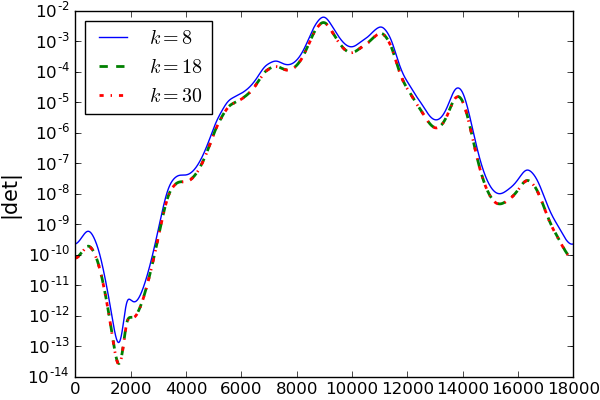
\includegraphics[width=0.6\textwidth]{ppo147det_2}
    \caption{
$||\det(\cdots)||$ of leading $[k\times k]$ block of the Floquet vector
matrix for the 147th \ppo. Compare with \reffig{fig:smallestAngle}
principal angle oscillations for the same \ppo. The big deal is that this
plot is computed as a `$k-form$', without any norm - it is intrinsic to
the linearization of the orbit.
    }
    \label{fig:ppo147det}
\end{figure}

  \begin{figure}[h]
    \centering
    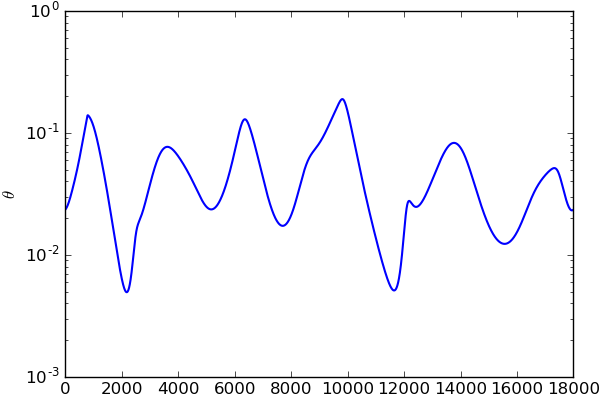
\includegraphics[width=0.6\textwidth]{ppo150MinAng}
    \caption{
    Angles along 150th \ppo\
    Compare with \reffig{fig:smallestAngle} oscillations
    for 147th \ppo.
    }
    \label{fig:ppo150}
  \end{figure}

\item[2016-03-15 Kazz to Predrag]
Remedy to your first two ulcers...

About point 1: The term ``local exponent'' is often used in the literature and it is in any way local in phase space, too, as it is simply obtained with the stability matrix and the covariant/Floquet vector, both of which are functions of phase-space point (though the vector carries information from the entire trajectory, so not a local quantity in this sense.). However, if you insist, I'm okay about the term ``instantaneous exponent'' too.
\\ {\bf 2016-03-15 Predrag} We'll probably stick with ``local'' exponent in this paper.
Not so important.

About point 2: The angle we show in the paper is the principal angle between two subspaces (or between one subspace and one vector), which is by definition non-negative. Even if you talk about the angle between two Floquet/covariant vectors, the sign of the angle doesn't matter, because the sign of the Floquet/covariant vector is arbitrary.

%I consider we don't need to introduce the strain rate tensor $D(x)$ in
%that way. Why do you ignore my remark that $A$ is real in our problem?
%(so $A=D$) Why did you remove the definition of $A$, which is in any way
%necessary? I'm afraid I don't think the manuscript is improved.

\item[2016-03-15 Predrag to Kazz]

\begin{enumerate}
  \item[(2)]
Yes, the way you think, all angles are positive. It's OK for this paper.
  \item[(3)]
%$\Mvar$ is defined earlier in the text (before the Jacobian is
%   defined) in the century old way, nothing to worry about. But I kept
%   your $\lim_{\tau\rightarrow 0}\lambda_j^\tau(\ssp)$, to emphasize why you
%   think of that as a `local' exponent.

%I answered your query about complex `local' Floquet exponent above, in
%the {\bf 2016-03-08} discussion: ``\PCedit{(Predrag: $\Mvar$ is real, but
%eigenvectors may be complex. 	Do not worry about, it's just a detail in
%our manuscript.)}. Don't you feel good that something that you have
%invented Landau and Lifshitz\rf{Landau59a} have also thought of, and gone
%to the trouble of finding out what it is called in continuum mechanics,
%so you do not have to make up a new name for it? It makes it easier on
%the reader to look up, if she does not understand our definition.

The way \cLvs\ are currently computed, only real Lyapunov exponents can
be computed, in accord with your own experience. However, Floquet
exponents give you both the rotation and the stretching / squeezing information.
Whether an instability is hyperbolic or spiral-out (complex pair) is very
important (overdamped / underdamped oscillator), and Xiong, Burak and I
discuss that daily: the whole \KS\ $L=22$ attractor is shaped by it, and
so are presumably oscillations clearly seen in peaks in
\reffig{fig:smallestAngle}. Those are a nuisance: they are the source of
these singularities poking out of the angle density histograms, something
one would like to get rid off.

These considerations are a part of
Xiong's thesis, and not a part of our PRL draft, which has a nice story
to tell as is.

\end{enumerate}

%\item[2016-03-16 Kazz to Predrag]
%
%I realized that what I wrote above on the matrices $A$ and $D$ was wrong.
%I'm sorry about this.
%
%I'm also okay about the obvious fact that the Floquet exponent can be
%defined as a complex number, and I do appreciate the importance of the
%imaginary part of the exponent. What I was saying is that, the definition
%given in our paper corresponds to the real part of the exponent, and it's
%sufficient for the purpose of the paper. In some previous version of the
%manuscript, it looked to me as if the exponent defined by the log of the
%modulus were a complex number, but now this problem seems to be resolved.

\item[2016-03-16 Xiong]
I \reffig{fig:ppo147proj}\,(left) which shows the $k=1,2$ Fourier components
of the 147th \ppo\ in full \statesp.

I try to think about Predrag's suggestion of using angle in range
$(-\pi/2, \pi/2]$ to take account of the fact that one Floquet
vector may cross the 2-dimensional plan spanned by other 2 Floquet vectors.
But this does not happen. Here is how I tested it. Numerically, I only
calculated the leading 30 Floquet vectors each of which has dimension
62, so I only got the first 30 columns of the Floquet vector matrix.
I assume that the other 32 Floquet vectors are pure Fourier modes,
so the determinant of Floquet vector matrix is the same as the
determinant of its leading $[30\times 30]$ block. The determinant
is a signed volume of the parallelogram formed by all Floquet vectors.
If one Floquet vector crosses the hyperplane spanned by other Floquet vectors,
then the determinant will change sign. What I found is that for
all 200 ppos, the sign does not change along the orbit.

I think this is reasonable otherwise the system changes from
left-hand system to right-hand system during time evolution.
Therefore, we should not worry about pure positive angles.

\begin{figure}[h]
    \centering
    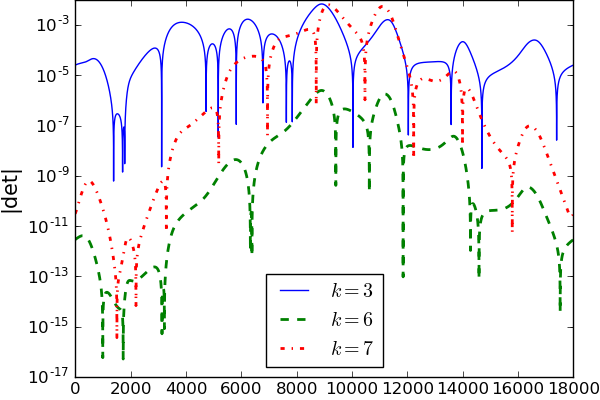
\includegraphics[width=0.45\textwidth]{ppo147det_1}
    \caption{Absolute determinant of leading $[k\times k]$ block
    of the Floquet vector matrix for small $k$, the 147th \ppo.
    }
    \label{fig:ppo147what}
  \end{figure}


By the way, I also try to calculate the determinant of the leading
$[k\times k]$ block of the Floquet vector matrix, which is the
volume projected onto $e_1 \wedge e_2\wedge \cdots, \wedge e_k$
direction. Here $e_i$ is the ith canonical basis. The result
for 147th ppo is shown in \reffig{fig:ppo147det}. Basically, adding
\transient\ modes does not change the volume. This may be profound,
because no arbitrary norm is imposed on the system (unlike the L2 norm
of angle measurements).

My interpolation may be wrong. I am not familiar with exterior algebra.

\item[2016-03-16 Predrag to Xiong]
Thanks for checking.
\begin{enumerate}
  \item
I guess this Fourier modes projections inclination is incurable. In your
code no \rpo s are projected on \statesp\ coordinates centered on and
aligned with some dynamical thing, like \reqva\ and their stability
eigenvectors? I do not expect wavenumber 6 oscillation to show up in the
1st and 2nd Fourier modes, so I am not sure that where the dots
land in projections of \reffig{fig:ppo147proj} reflects the true rotation
of this \ppo.
  \item
Does the angle you are measuring involve a leading complex Floquet
eigenvector? If so, is the imaginary part of the Floquet exponent
consistent with approx.
6 rotations per \ppo's period \period{150},
8 rotations per \ppo's period \period{147}?
  \item
\refFig{fig:tangency_ppo147} is the histogram of angles (computed by
counting points in horizontal strips in  \reffig{fig:smallestAngle}) for
\ppo\ 147. But what is the histogram of the angle shown in
\reffig{fig:histogram1}?
  \item \refFig{fig:ppo147det} is very nice!
  \item
What do you mean by ``$e_j$ is the $j$th canonical basis?''. Floquet
eigenvectors?
  \item
I am encouraged with all singular dips for small $k$ in
\reffig{fig:ppo147what}, and the fact that there are fewer of them as $k$
approaches the \entangled\ manifold threshold. Each dip might mean an
eigenplane crossing. By $k=7$ one is almost at \reffig{fig:ppo147det},
except for a few singular dips.
Fine detail will be needed, as well as precise formulas (gasp!)that
describe what is it taht you compute.
I presume you $L2$-normalize all Floquet vectors to 1; that cannot be
right, the right thing is to use Floquet theory to preserve their length
on average, over one period. The way you do it, presumably each
additional \transient\ eigenvector pair adds an `unit square' to the
dimensionality, thus not changing the value of the determinant.
  \item
I do not know of any reason why volumes spanned by would not change from
a left-hand system to right-hand system during time evolution. Actually,
if that happens, that would be wonderful, because you could associate an
integer index (the whole thing smells like Maslov indices) with each
orbit, and that would be a robust topological signature of the
\entangled\ manifold, much more persuasive than angle measurements.
  \item
Can you add a little subroutine to your $\phi(\zeit)$ plots, so that the
horizontal axis in figures is the time $\zeit$, not the number of time
integration steps? And enforce the width of the plot is given by
\period{p} in the same time units, so that shorter orbits are narrower?
If the oscillation is caused by the shape of the global attractor, longer
orbits will have more oscillations, proportional to the length of the
period.
  \item
In this context it would be good to state the period \period{p} of every
orbit plotted, besides its ordinal number in Ruslan's list (Matlab is not
running right now on my machine, so I cannot look up his data set).
  \item
You might not remember, but I have suggested using differential forms
often over the last 2 years. Essentially, we have evidence that each
orbit knows the inertial manifold dimension, suggesting that that
information is local (one does not need to measure distances between
separate orbits). The only local thing beyond the rate of growth of
Floquet vectors I can think of is the behavior of volumes defined by
their skew (exterior) products. Mohammad was receptive, so most of that
discussion ended in \texttt{svn elton} blog, you can check it out and
read it, there might be some interesting stuff there. Or ask Mohammad to
read this blog and give you input.

\end{enumerate}

\item[2016-03-18 Evangelos to Xiong] Your check for crossings using
the determinant is very interesting, but I think that I would need
equations in order to understand what you really do. So far I have
a naive question: For figures like \refFig{fig:ppo147det} is there
any chance that some numerical algorithm used in your calculations
takes advantage of the arbitrariness of the direction of eigenvectors
and uses some convention that causes the determinant to always be
positive? Or do you really track the advection of Floquet vectors
by the flow?


\item[2016-03-18 Xiong to Evangelos]
Right now the result is quite preliminary and I will test more
samples. I am preparing the answers to some questions raised by
Predrag, so I will update blog during the spring break.

For your concern that Floquet vectors may reverse direction
along the orbit, this scenario does not happen at least for \ppo s. The
\ped\ algorithm I am using guarantees that Floquet vectors are
transported along the orbit smoothly without sudden change of directions.
For \rpo s, it seems also true, but I need to verify because the two
marginal directions are exactly degenerate for \rpo s.

\item[2016-03-20 Xiong to Predrag]
  I just had a look at Roysoc16.pdf. It looks like a long talk with
  a lot of figures. 40 minutes may not be enough to reach to the
  dimension part. Good luck ! \\
  {\bf 2016-04-08 Predrag}: I managed to do it in 35 min ;).
  I incorporated the rest of your comments. I liked your eigenfunction
  figures, but had no space for them - will probably incorporate it
  into the online version of the talk.
  \begin{itemize}
  \item At slide 46 titled
    ``a relative periodic orbit: after symmetry reduction'',
    there shows two marginal Floquet vectors along an orbit, but this
    is in the full state space. Also, this figure is an old one which
    only shows accuracy $10^{-5}$.
    The one below is the new one used in Schur draft.
    \begin{figure}[h]
      \centering
      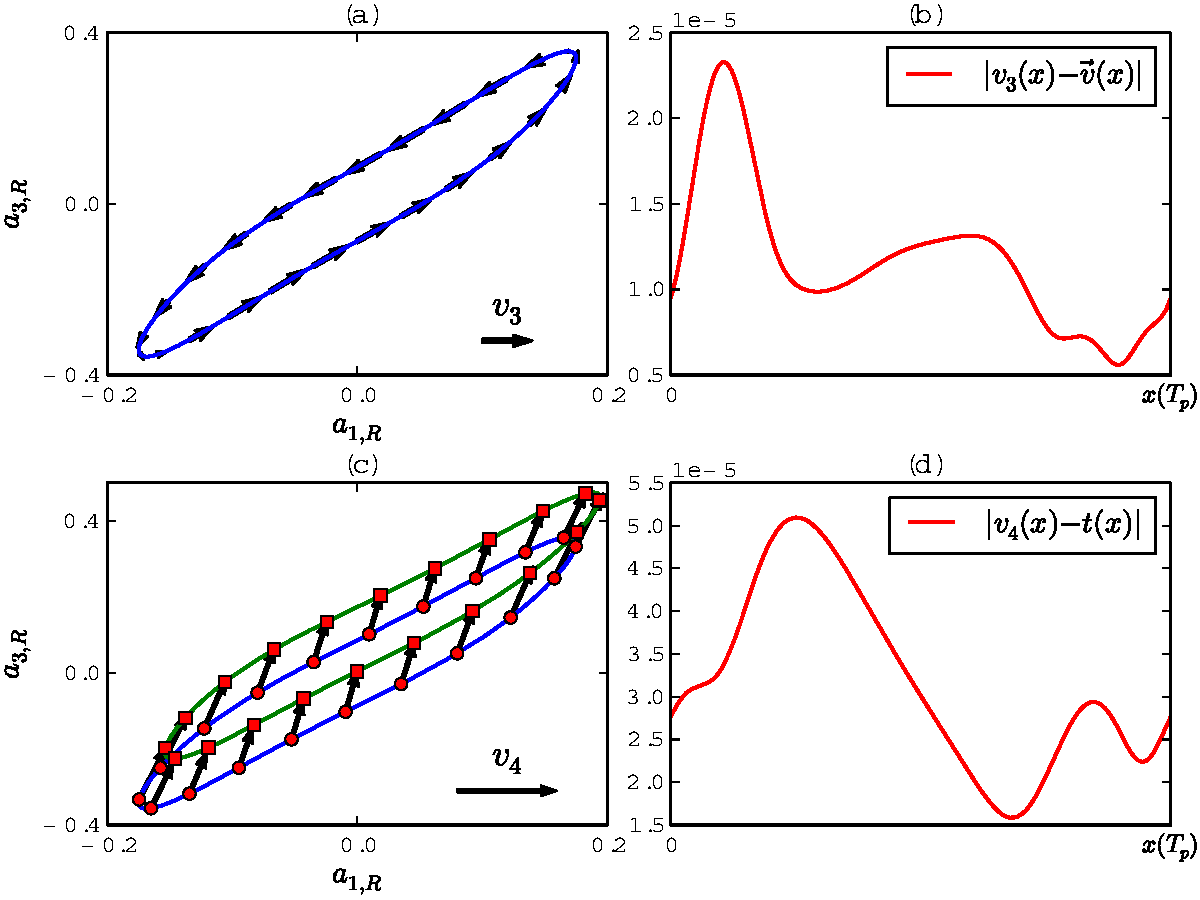
\includegraphics[width=1.0\linewidth]{ppo1vectfield}
    \end{figure}
    Also, if you want show more Floquet vector examples, I have some
    used in Schur draft too. \refFig{fig:Fvs} shows the evolution of
    Floquet vectors in one period.
    \begin{figure}[h]
      \centering
      \begin{minipage}{.115\textwidth}
        \centering \small{\texttt{(a)}}
        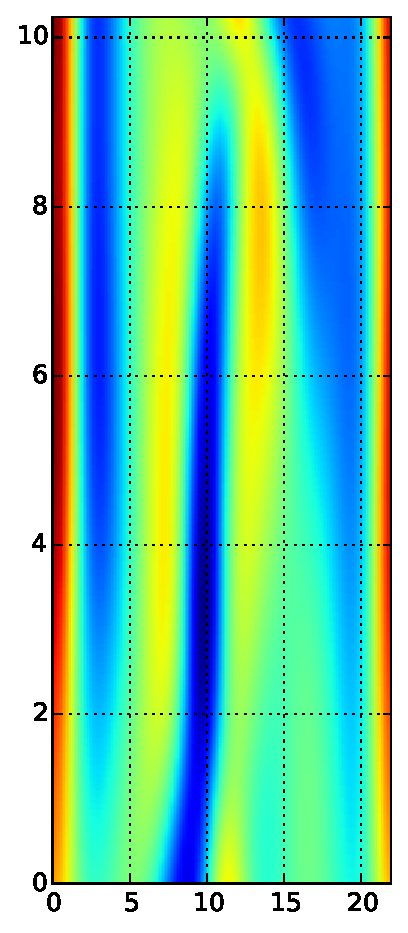
\includegraphics[width=\textwidth]{ppo1Fv1_64}
      \end{minipage}
      \begin{minipage}{.115\textwidth}
        \centering \small{\texttt{(b)}}
        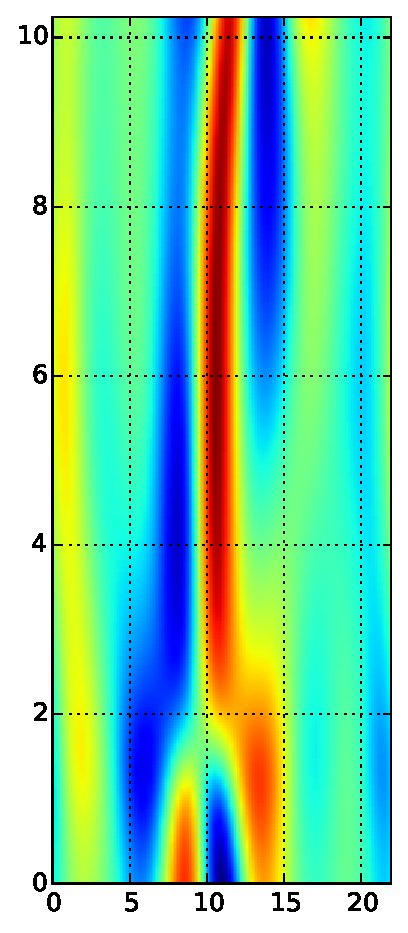
\includegraphics[width=\textwidth]{ppo1Fv5_64}
      \end{minipage}
      \begin{minipage}{.115\textwidth}
        \centering \small{\texttt{(c)}}
        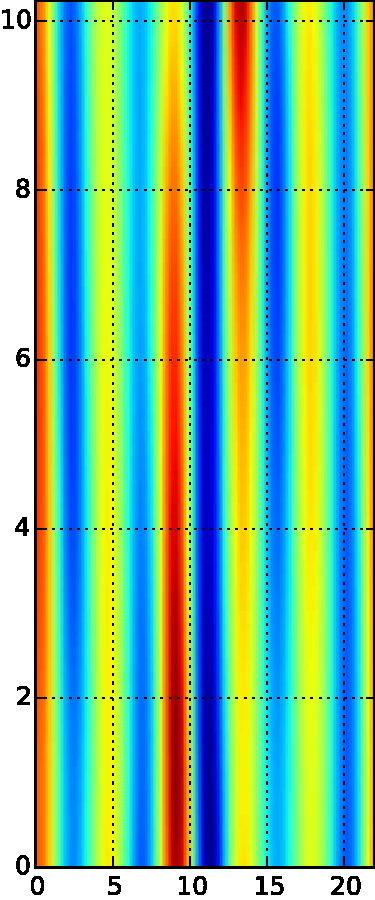
\includegraphics[width=\textwidth]{ppo1Fv10_64}
      \end{minipage}
      \begin{minipage}{.115\textwidth}
        \centering \small{\texttt{(d)}}
        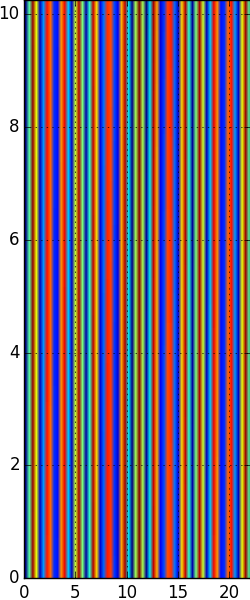
\includegraphics[width=\textwidth]{ppo1Fv30_64}
      \end{minipage}
      \begin{minipage}{.115\textwidth}
        \centering \small{\texttt{(e)}}
        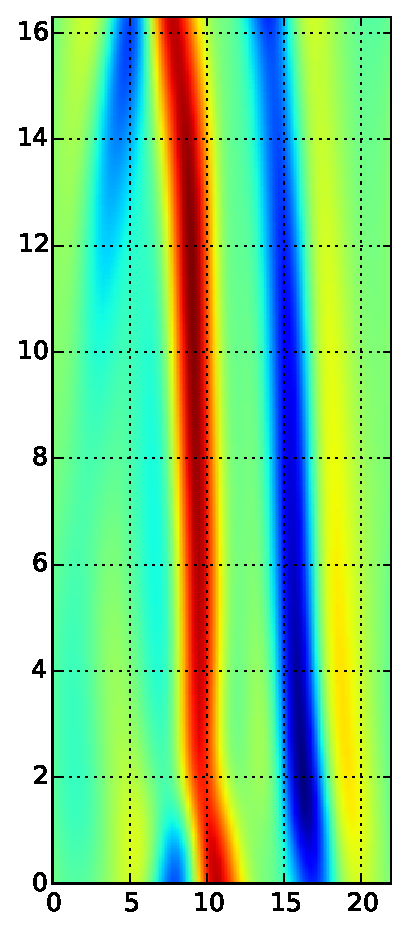
\includegraphics[width=\textwidth]{rpo1Fv1_64}
      \end{minipage}
      \begin{minipage}{.115\textwidth}
        \centering \small{\texttt{(f)}}
        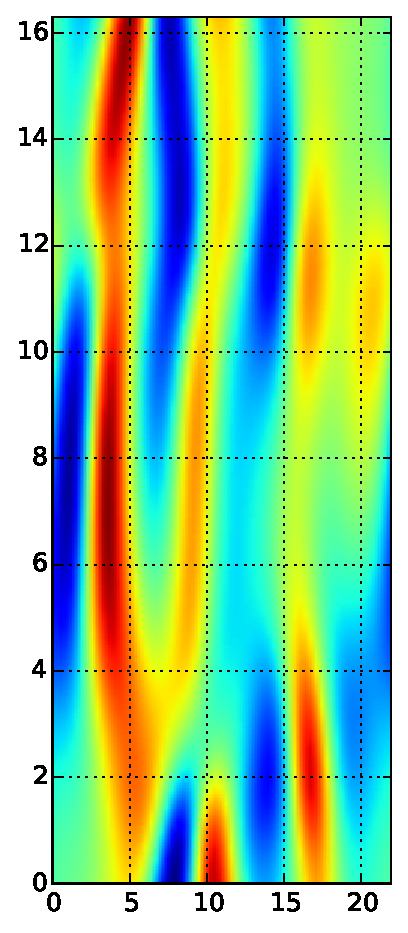
\includegraphics[width=\textwidth]{rpo1Fv4_64}
      \end{minipage}
      \begin{minipage}{.115\textwidth}
        \centering \small{\texttt{(g)}}
        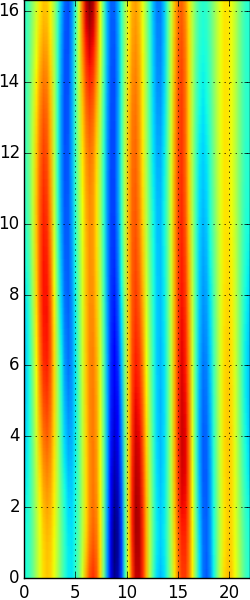
\includegraphics[width=\textwidth]{rpo1Fv10_64}
      \end{minipage}
      \begin{minipage}{.115\textwidth}
        \centering \small{\texttt{(h)}}
        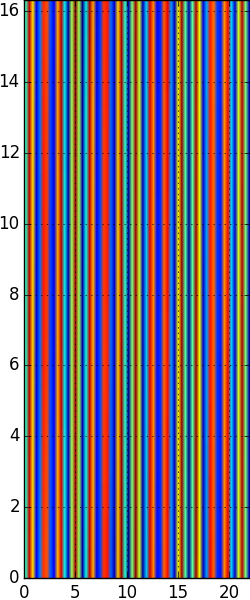
\includegraphics[width=\textwidth]{rpo1Fv30_64}
      \end{minipage}%
      \caption{(Color online)
        (a) $\sim$ (d) : the 1st (real part), 5th, 10th and 30th \Fv\ along
        $\cycle{pp}_{10.25}$ for one prime period.
        (e) $\sim$ (h) : the 1st, 4th (real part), 10th (imaginary part) 30th (imaginary part)
        \Fv\ along $\cycle{rp}_{16.31}$ for one prime period.
        Axes and color scale are the same as \reffig{fig:ppo1rpo1}.
      }
      \label{fig:Fvs}
    \end{figure}

  \item The figure at slide 56 titled `` Kuramoto-Shivashinsky L = 22
    small cell '' does not look good enough. Also the same spectrum is
    covered at slide 58.

  \end{itemize}

\item[2016-03-21 Evangelos to Predrag] I had a look at the Roysoc16 presentation.
I think it is similar to the one you gave in Dresden except for the
addition of the Floquet part. This means that you would be stressed to
talk about all this in 40 minutes so you might wish to reduced some part
(something that your audience will be familiar with). Your six claims
seem true to me. I am not sure if the people will get what a separation
vector is. Maybe there is some sketch of it already that you could use?

\item[2016-03-21 Evangelos to Predrag]
I think that by making the choice not to cite any papers you don't use the
opportunity to inform the audience that although this program sounds very hard to
realize, there are now several papers that make progress towards that goal.
The other problem is that it makes it harder for the interested person
at the audience to look something up. (One extreme example is citing Cartan
for slicing... I think that if somebody read his papers he would still not
know how to slice...). Anyway I think that you have specific reasons to follow
this approach (reaction from people that are not cited?).

\item[2016-04-08 Predrag to Evangelos]
In the 40 min talk there was no time to go into references, so I
apologized verbally at the beginning of the talk. But you are right. In
the online pdf file of the presentation, I will add the references.


%\item[2016-03-25 Xiong to Predrag and Kazumasa]
%For the new draft of dimension paper, I find two places weird. \\
%    1. The middle part of the 2nd page. ``62 real modes(62-dimensional
%    state space)''. Should 31 Fourier modes (62-dimension state space)
%    sound better ? \\
%    2. The bottom part of the 2nd page. `` DOS refers to of '' is a
%    broken sentence.
%  Predrag 3016-03-27 fixed

\item[2016-04-08 Predrag to Xiong] Almost every line in bib entry for
Havard Berland, Brynjulf Owren, and Bard Skaflestad\rf{Berland05}
(amazing Norwegian names) had to be edited, and DOI was missing. But you
do not seem to cite it anywhere? Looks like it needs to be described,
cited in \refsect{sect:RKadapt}.

They consider
\beq
u = Lu + N ( u ) ,u (0) = u_0
\,.
\ee{Berland05}
Their order theory is valid for a class of exponential integrators,
including the Runge–Kutta–Munthe-Kaas (RKMK) schemes\rf{MuntheKaas99}, the
commutator-free Lie group integrators\rf{CeMaOw03}, and schemes of Cox and
Matthews\rf{cox02jcomp} and Krogstad\rf{Krogstad2005} which reduce to
classical Runge–Kutta schemes when $L =0$.

\item[2016-04-08 Predrag and Xiong to all] We are planning to ask people
listed below to have a look at our paper. Who else?

To : G. Radons <radons@physik.tu-chemnitz.de>,
     F. Ginelli <francesco.ginelli@abdn.ac.uk>,
     Hongliu Yang <hongliu.yang@physik.tu-chemnitz.de>,
     Antonio Politi <politi@inoa.it>,
     Christopher L.P. Wolfe <clwolfe@ucsd.edu>,
     Roger M. Samelson <rsamelson@coas.oregonstate.edu>,
     Harald Posch <harald.posch@univie.ac.at>,
     Ulrich Parlitz <parlitz@physik3.gwdg.de>,
     Pavel Kuptsov <p.kuptsov@rambler.ru>,
     Nikolay V. Kuznetsov <nkuznetsov239@gmail.com>,
     Masanobu Inubushi <??>,
     Charlie Doering <doering@umich.edu>,
     Peter Constantin <const@math.princeton.edu>,


Dear Professor **,

Over past 2 years I have, guided by P. Cvitanovi\'c, K. A. Takeuchi,
E. Siminos and H. Chate, carried out a number of numerical experiments
to check whether periodic orbits of the Kuramoto-Sivashinsky system can
be used to determine the dimension of its inertial manifold. On the
whole, it appears that such methods might enable us to construct the
inertial manifold by tiling it with linearized neighborhoods of
(relative) periodic orbits.

The current version of our work is available on
http://arxiv.org/abs/1604.01859

I would be grateful for any comments, suggestions, criticism or pointers
to work we might have overlooked.

Sincerely,

\item[2016-04-13 Xiong]
I sent out the emails to the above professors, 4 of which failed to deliver:
Hongliu Yang <hongliu.yang@physik.tu-chemnitz.de>, \\
Christopher L.P. Wolfe <clwolfe@ucsd.edu>, \\
Antonio Politi <politi@inoa.it>,\\
Ulrich Parlitz <parlitz@physik3.gwdg.de>,

\item[2016-04-13 Xiong]
New emails:
Antonio Politi <a.politi@abdn.ac.uk>,\\
Ulrich Parlitz <ulrich.parlitz@ds.mpg.de> \\
But still could not find Hongliu Yang and Christopher L.P. Wolfe.

\item[2016-04-14 Xiong to everyone] I received feedback from F.G. Ginelli.
Here is the content of email.

\renewcommand{\edit}[1]{{\color{red} #1}} % edits to implement in the draft


\begin{quotation}

Dear Xiong \& Hugues,

I have to say I find your paper really interesting. The ideas put forward
are really nice, and your results are surely something to think about
carefully (indeed I had to digest your paper a little bit and re-read
it at least once).

For instance, I was initially surprised by the fact that ALL po have the
same number of physical modes, but this could be natural if you think that
they have to be contained in the inertial manifold, and that it is not
unlikely to think that po
living in a lower dimensional subset should be quite unlikely
(something like zero-measure?). You say something about this in
the conclusions, but maybe you could comment more explicitly on this point.

Also, it seems to me that your results imply (or assume?) continuity over
the attractor of the covariant vectors (or better
put of the Oseledets splitting structure). This is always a delicate point
 maybe worth discussing. I know that Gary Froyland
form UNSW Australia is working on this and he could be really interested in
your results. There are a few  (mostly
mathematical) papers where these continuity issues are discussed, but I am not
sure the hypothesis they put forward are
meaningful for dissipative systems:

The Ershov and Potapov one in Physica D 118, 167 (1998)
and these two references given to me by Gary Froyland:\\
http://jlms.oxfordjournals.org/content/early/2015/12/07/jlms.jdv057.abstract
http://web.maths.unsw.edu.au/~froyland/semi-inv-holder-cty\_16final.pdf \\

Apart from this, I have a few questions/comments (maybe more later):

1.
When in Fig. 3 you test the separation vector between the chaotic and the
periodic orbit (BTW, I think there is
    \edit{
a typo two
lines after Eq. (6), it should be $w_n$ and not $w_k$ ),
    }
Fig. 3c and 3e nicely
 confirm the bounding of the angle by the separation norm for $n>=7$.
However, I wonder why in Figs. 3d and 3f the average angles for $n>=17$ show
clear deviations
from a linear behavior at small separation values. Is it just an accuracy issue?


2.
If I understand well your local Floquet exponents, it is really an
 instantaneous object. Your results in Fig. 1b-c clearly show that something
 drastically different is going on between
exponents 1-8 and the rest. This is perfectly convincing to me.
However, the fact that you are using the $\tau \to 0$ limit puts you out of the domain of the
Bochi and Viana dominated splitting results, and maybe you should be more clear about this.

I wonder if one could get a little bit more rigorous (and close to the
 dominated splitting result by B\&V) by considering --
like you are doing with angles in Fig. 2 -- ensembles of pos.
What I mean is: if, for each orbit p of period $T_p$, you compute the
smallest time $\tau_m$ such that the first 8 finite time
exponents $\lambda_i^tau_m$ are dominated, and then you consider the distribution
 of these $tau_m/T_p$ values over all periodic
orbits, what are you going to see?
Could it be that this distribution is NOT clearly  bounded away from 1? These I think
would reconcile your results with B\&V.
But this is just a curiosity, I am not at all implying you should also add this to
your already impressive paper.

3.
One curiosity: In the caption of Fig. 1 you specify that the 4th LE is small but
strictly negative,so that you would only have 1 positive exponent (and 2 zero ones).
This is clearly the case for the rpo 16.31 while your ppo 10.25 numerics seem to give
 a positive second LE with a zero 3rd and
4th ones. The fact that for this orbit the first 2 LEs are nonzero (and practically identically)
 is also confirmed by Fig. 2c,
where their instantaneous Floquet exps looks really the same!
Is this just a problem of numerical accuracy or do you think there is some dimensional
variability at play? Did you had a look at some other periodic orbit for this?

4.
If I understand correctly what you are doing, I think Eq. (5) could be slightly
clearer if you write the po term as $u_p(x +
t_p)$ where $0 \le t_p<T_p$ is some phase shift along the orbit to minimize the in-slice distance.

Anyhow, it is really a nice work, congratulations...

Cheers

Francesco

\end{quotation}

\item[Xiong 2016-04-14]
I initialize a reply to Prof. Ginelli.

\begin{quotation}
  I do not think the continuity of covariant vectors is a concern, which is
  indicated by Prof. Ginelli. The paper he methioned `` Physica D 118, 167(1998)"
  \rf{ErshPot98} talks about the limit of $J^TJ$. The result in this paper
  is important for computation of Covariant Lyapunov vectors. But for a
  perodic orbit, the Floquet vectors are calculated by following the orbit
  for only one period. The continuity of Floquet vectors is naturally ensured
  by the Floquet vector algorithm. The only examption I can think of is that
  the instantaneous velocity derivative (stability matrix) is ill-behaved.
\end{quotation}
[Kazumasa 2016-04-15]
Basically I agree, but for the periodic orbits there are two points
here: continuity of Floquet vectors along an orbit, and continuity of
Floquet/Lyapunov vectors at two nearby points (not on a single
orbit/trajectory). While I feel okay about the first point (like you),
but I guess Francesco's remark is more related to the second point,
which is indeed delicate and I guess we don't have any argument about
it, apart from our numerical observations.

\begin{quotation}
  For point 1, thanks for pointing out the typo. For average angles
  with $n \le 17$ in Fig3.d and Fig3.f, I guess you are referring
  to the dip between $||\Delta u|| = 10^{-2}$ and $||\Delta u|| = 10^{-1}$.
  The reason is very simple. On the attractor, long wave states dominate
  short wave state. so when two points are far away, their difference
  still have structure similar to long waves. Also, the leading
  7 in-slice Floquet vectors all have long waves structure, and the
  remaining in-slice Floquet vectors are almost sinusoidal waves
  (Fourier modes), so the difference vector can be expanded well
  by the leading 7 vectors. You can think of it in Fourier modes.
  Let $a_k$ is $k$th Fourier mode. On the attractor, $a_k$ with small
  $k$ has large magnitude, the same with difference vectors if two states
  are far away. The leading 7 in-slice Floquet vectors are concentrated
  on the first few Fourier modes.
\end{quotation}
[Kazumasa 2016-04-15]
Sorry, I didn't understand how this argument answers Francesco's
question. He's asking about reasons why the angle doesn't seem to decay
linearly for n >= 17 (brown, green, violet symbols). Myself I don't know
why, but what we believe is that those data points also eventually decay
linearly with $||\Delta u||$ for smaller $||\Delta u||$, as those for n
closer to the threshold do. It's also important to remind that, by
definition, $\varphi_n <= \varphi_m$ for $n>m$, so the data for n >= 17 are
always bounded by those for n=7 which do decay linearly. I think it's
better to argue these points.


\begin{quotation}
  For point 2, I am not quite sure about the concern. I will discuss it with
  other coauthors. But our result shows that no matter how small you chose $\tau$,
  the leading 8 $\lambda_i^\tau$ always dominate. There is no need to draw
  some distribution.
\end{quotation}
[Kazumasa 2016-04-15]
Read again what we (I) wrote about DOS in the manuscript: usually
finite-time exponents are related to hyperbolicity when the averaging
time is large. In constrast here we take the opposite limit (i.e.,
instantaneous limit) and argue relation to hyperbolicity. I guess it's
difficult to justify this choice from the theoretical viewpoint. In my
opinion we should simply report what we found numerically (and discuss
the contrast with the usual approaches based on DOS), without making a
speculative connection between them.

\begin{quotation}
  For point 3, ``4th LE is small but strictly negative''. This is true.
  But this fact about Lyapunov exponents does not imply that there is
  only one positive Floquet exponent (I meant its real part) across all
  relative/pre-periodic orbits. Some orbits have only one unstable direction.
  Others have two. Lyapunov exponents are long time average over the attractor,
  not for a specific orbit.
\end{quotation}
[Kazumasa 2016-04-15]
Good, but I suggest you also remark that the first two positive
exponents of the orbit in question come from a pair of complex
conjugates of the corresponding Floquet multipliers.

\begin{quotation}
  For point 4, thanks for your suggestion. but there may be a typo
  in the email. I guess you want to say $u_p(x, t_p)$ not $u_p(x+t_p)$.
  After reducing SO(2), relative periodic orbits become periodic with period
  $T_p$, but pre-periodic orbits still have period $2T_p$. So numerically, I
  search $u_p$ for one period for a relative periodic orbit, but one period
  and its reflection for a pre-periodic orbit. I am not sure such detail should
  be written explicitly in this paper.
\end{quotation}
[Kazumasa 2016-04-15]
I guess he suggested to use $u_p(x + t_p)$ instead of $u_p(x; t_p)$, but I don't
think it makes a big change, and I prefer our choice, which looks simpler.

\renewcommand{\edit}[1]{{\color{blue} #1}} % for referees


\item[Xiong 2016-04-19]
I attached a pdf version of the above {\bf [2016-04-14]} post as  the
reply to Prof. Ginelli, and I made no edits whatsoever in the draft of
the article.

\item[2016-04-28 Hugues]
Note that if you stretch a bit the results of our PRL submission, one
could dream of getting an estimate of the manifold dimension from just a
few of the `exact coherent structures' your fluid-dynamics friends are
collecting.

\item[2016-04-28 Predrag]
If it is really true that individual periodic orbits suffice to estimate
the inertial manifold dimension, we are in heaven. I fear that the PRL
results might be specific to Kuramoto-Sivashinsky, which is atypically
nice due to the hyperdiffusivity (Laplacian$)^2$.

The problem is that with the current technology we can compute max 30
Floquet vectors for plane Couette, less for the pipe, and that is not
sufficient. Xiong's periodic Schur works up to 100 dimensions or so, on
short \po s, but in fluid dynamics we are in minimum 100,000 dimensions,
so one has to replace Jacobians in Schur decomposition by numerical
Krylov spaces, and combining this with Schur (many points around a
periodic orbits) is at present terra incognita. There is not enough time
for Xiong to attempt that - it would really require a postdoc and
commitment to several years of work, and where do you find a person like
that?

Whether one can scale up the covariant Lyapunov vector methodology to
100,000-dimensional flows only you know - the high quality integrators
you can download from Channelflow.org and Openpipeflow.org, but the
adjoint part of the evolution I think would require serious work, and how
well will Oseledec converge with ergodic trajectory length in such high
dimension I do not know.

I remain optimistic, but it will take more manpower, and more than 8
months to get any results, I think.

\item[2016-05-02 Xiong to Predrag] For high dimensional systems, \psd\ is
surely not appropriate. But the periodic Krylov-Schur algorithm by
Kressner\rf{Kressner2006} from renowned EPFL may be most
promising solution from my point of view. I once asked Daniel  Kressner
for the code. But he said it is lost. I guess he has a preliminary
version but not well tested, so he does not want to share with others.

\item[2016-05-02 Xiong] I got reply from Nikolay V. Kuznetsov
about the dimension draft.

  \begin{quotation}
    Dear Xiong,

    Thank you for the paper.
    As a  matter of fact, I had found it a day before your e-mail. I
    thought how to connect your approach with our analysis of dimension,
    but up to now without progress :(

    WBR	

    Nikolay
  \end{quotation}

He also attached his {\em The Lyapunov dimension and its estimation via
the Leonov method}\rf{Kuznetsov16}. I will try to read it.

\item[2016-05-02 Xiong]
I had a quick glance of Kuznetsov's paper. He tries to get the local
Lyapunov dimension from invariant sets but without finding these
invariant set. It sounds like using periodic orbits but not trying to
find them.  Since its definition is closely related to Kaplan-Yorke
dimension by using singular values of finite time Jacobian, its purpose
is to estimate the dimension of attractor. I think this is the biggest
difference compared with dimension draft. We try to get an integer number
of the inertial manifold.

I have not replied to him as yet.

\item[2016-05-02 Predrag to Xiong]
I have noticed Kuznetsov's most recent paper\rf{Kuznetsov16}, but had not
entered it here, as I previously had asked you to read
\HREF{http://arxiv.org/find/nlin/1/au:+Kuznetsov_N/0/1/0/all/0/1}
{N. V. Kuznetsov} papers (see {\bf [2014-10-16 Predrag]}, {\bf
[2015-08-29 Predrag]}, {\bf [2015-09-25 Predrag]}, and {\bf [2015-10-14
Farizmand]} above).

I am quite sure that Lyapunov did not invent ``Lyapunov dimension''; as
explained in your thesis, we refer to this dimension as the Kaplan-Yorke
dimension\rf{KapYor79a,FKYY83}, and it seems to be about 1/2 of the
inertial manifold dimension. You discuss this above in
\refsect{sect:varDims}, \texttt{dimension.tex}, and you absolutely need
to explain these dimensions in your thesis, so why don't you seriously
reexamine/edit your own notes, and then explain  to Kuznetsev what
different dimensions are? In particular, that ``Lyapunov dimension'' is
way off, that the important dimension is the inertial manifold dimension.
Or whatever we call it. As almost everybody mistakes the Kaplan-Yorke
dimension for what we do, you must be ready to explain the difference
whenever this happens.

It's you PhD thesis, you know this stuff better
than anyone, so stand your ground!

\item[2016-05-08 Xiong to Predrag]
This may sound like nonsense.
I am thinking of some idea about ``directional fractal dimension''.
The reason goes as follows.
There is humongous literature on the dimension of an strange attractor,
like box-covering dimension, information dimension, correlation
dimension, Lyapunov (Kaplan-Yorker) dimension  and so on and so forth.
They all give me an impression that they are a summation of fractal
dimension in each direction. So, I have a conjecture
\[
  \sum_{i=1}^n d_i = D_B\,,\quad  0 \le d_i \le 1
\]
With $D_B$ the box-counting dimension.
But immediately there is a problem.
For example, in the following picture,
\\{\centering
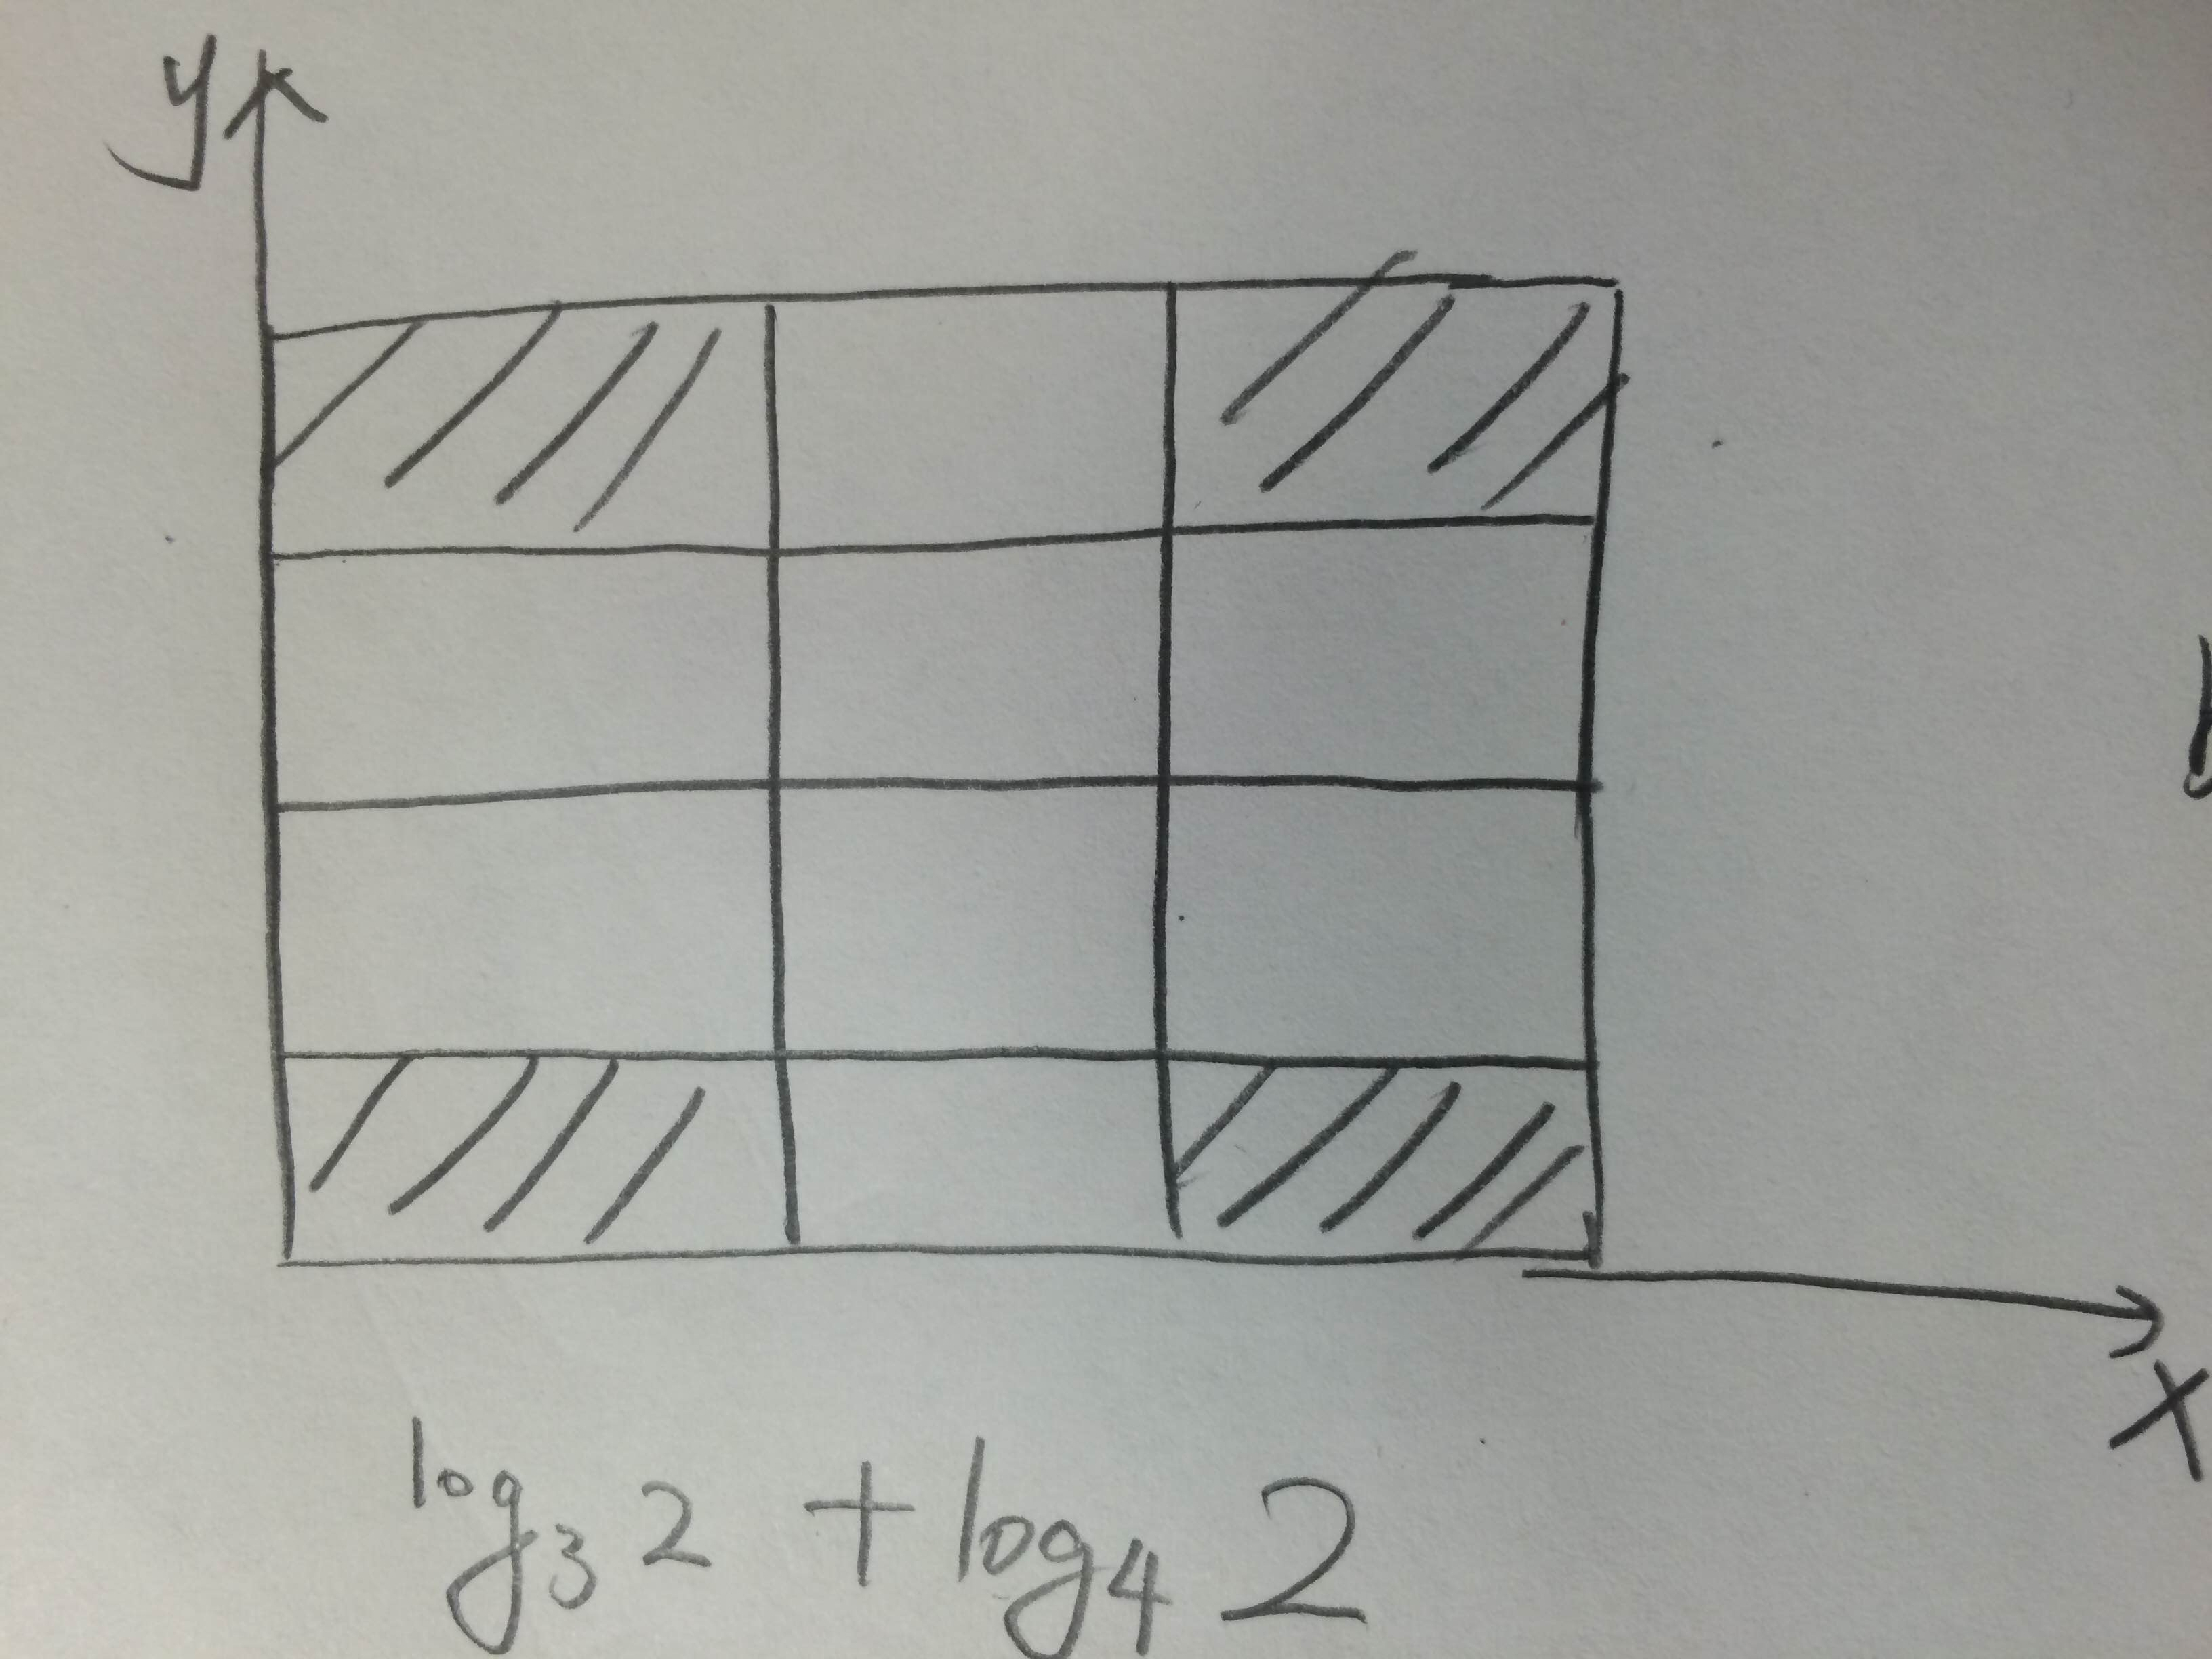
\includegraphics[width=0.3\textwidth]{dimenFrac}
}\\
we divide the x-axis in 3 equal pieces and y-axis in 4 each pieces,
and keep doing it in the 4 edge regions.
I thought the box-counting dimension is
$\log_32 + \log_42$. But it seems not true.

\item[2016-05-08 Predrag]
In your thesis you should 1st explain, very briefly but correctly
various `fractal' dimensions popular in 1980's, and then explain why
they are no good for your problem (`dimension of turbulence').

                                                            \toCB
First of all, fractal dimension is an example of an easy idea to explain
in 1 dimension (a Cantor set) which gets harder and harder to justify in
a few dimensions, and is soon seen to be a cheap but totally useless
idea. That's the reason that I barely cover it in ChaosBook. Eckmann and
Ruelle\rf{EckmannRuelle1992} explain very clearly in {\em Fundamental
limitations for estimating dimensions and {Lyapunov} exponents in
dynamical systems} why there is no chance to measure any dimension higher
than 8 (and in practice much less).

All these dimensions are stupid, because they look at a fractal as
a static object, and try to cover is with sets of balls or boxes of
various sizes. But in dynamics, fractal is a consequence of the basic
dynamical operation (stretch and fold), so --as explained in ChaosBook--
for the simplest examples you can compute dimension exactly from one-step
dynamics (eigenvalues of the {\FPoper}), no need for any box counting.
And in higher dimensional flows, covering with boxes does not make sense,
as it has no natural dynamical motivation or implementation.

You want to compute only \emph{observables}, but only way to `measure'
static fractal sets is by computers talking to computers, they are in no
sense observables of long-time dynamics. Mathematicians have defined
Hausdorff dimensions as a mathematical invariant characterization of a
fractal set, but the rigorous notion is of no use to us, as it cannot be
measured by any macroscopic physical measurement (unlike, let's say,
friction on the wall of a pipe, or mixing rate of a turbulent flow).

It's not worth too much of your time, but back to your Cantor set example:
Along the $x$ axis, the Hausdorff dimension is $d_1 = \ln(2)/\ln(3)
\approx 0.631$, and along the $y$ axis $d_2 = \ln(2)/\ln(4)$, and they do
add. Is the problem for you that the boxes are not squares but rectangles?
If you cover it with squares of size $L/4$, it does bad job along th
$x$-direction, but it should converge to $d_1$ in the limit.
We agree?

But in dynamical systems the idea is that along every unstable direction
the measure is continuous (it gets stretched and smoothed out) so the
dimension is exactly one 1. Along the contracting directions you get a
fractal dimension $0 < d_i < 1$, due to every fold being insufficiently
thin to fill up the unit interval. As long as everything is hyperbolic:
look at the pictures of the H\'enon and Lozi attractors. But in higher
dimension the directions are nonlinearly coupled, and the strange
attractor does not decompose in anything simple along each linear
coordinate.

Kaplan-York hunch (purely heuristic, no rigor of any kind) is that as
long as $m$-dimensional parallelepiped keeps getting stretched (sum of
the stability exponents for the first $m$ expanding directions is
positive), there are $m$ integer dimensions - and then they have an
argument that the leftover gives a fractal bit, generalizing from what we
understand about the 2\dmn\ H\'enon attractor. In retrospect, it is very wrong
in the few PDEs that have been studied so far.

None of `fractal' hand-waving is worth much, the covariant vector
dimension of the inertial manifold I find much more persuasive.

\item[2016-05-16 Predrag  to Xiong]                         \toCB
Can you do a quick read (and blog about it here) of M. Sandri\rf{Sandri96}
{\em Numerical calculation of {Lyapunov} exponents}. I think the
Mathematica routine is based on this, I wonder how good (or wrong) is it.
To me, looking at its references, it looks suspect. And is
Ramasubramanian and Sriram\rf{RamSri00}
{\em A comparative study of computation of {Lyapunov} spectra with
different algorithms} any good?

\item[2016-05-17 Xiong]
Sandri\rf{Sandri96} presents the method Mathematica uses in computation
of Lyapunov exponents. The paper recapitulates many important concepts in
dynamical systems, like $\omega-limit$ set, attractor, periodic motion,
chaotic motion, Hausdorff dimension, Lyapunov exponents and so on. The
algorithm follows Benettin \etal\rf{bene80a}. Overall, it is an easy and
good introduction to this subject. However, the statement at the end
about Lyapunov dimension that ``$D_L$ is a lower bound of capacity
dimension'' is not correct. Actually, it is an upper bound.

\item[2016-05-16 {\`A}ngel Jorba, Predrag, Xiong]
Talked about what happens when stability eigenvectors are exactly
parallel, but the stability multipliers are distinct. {\`A}ngel
says that for a \po\ they can be arbitrarily close to being parallel,
but the Floquet theorem guarantees that they cannot be \emph{exactly}
parallel (degenerate). He also finds our probability density function
being flat for small angles\rf{DCTSCD14} counter-intuitive.

Predrag worries that if a pair of stability eigenvectors is nearly
parallel, but expansion/contraction rates are different, the neighborhood
between the two must get weirdly deformed. Jorba, Tatjer, N{\'{u}\~{n}ez}
and Obaya\rf{JorTaNuOb07} {\em Old and new results on strange nonchaotic
attractors} have nice examples of very wild things going on, but setting
is different: they study invariant curves of 2+1/2 maps (external
periodic forcing, so these are essentially \PoincSec s of 3\dmn\ tori.
Their stable/unstable manifolds have different eigenvectors at every
point of the invariant curve, and when these touch, things go crazy - see
figures in the paper\rf{JorTaNuOb07}.

\item[2016-05-23 Xiong] We get feedback from Prof. R. M. Samelson.
  \begin{quotation}
    Many thanks for sending your interesting manuscript.  I am sorry for
    the slow reply.  You might be interested to know that, along with
    your reference 10, there was an alternate method of obtaining the
    characteristic Lyapunov vectors proposed independently and nearly
    simultaneously\rf{WoSa07}: Wolfe, C. L., and R. M. Samelson (2007
    {\em An efficient
    method for recovering Lyapunov vectors from singular vectors}.

    The two methods have been compared by Kuptsov and Parlitz\rf{KuPa12}.
  \end{quotation}
  He mentioned his work of calculating \cLvs. We know it but did not cite
  it in the draft because Ginelli \etal's algorithm is used instead.

\item[2016-05-23 Predrag] Samelson is right, pity he has no comments on the
paper itself. When you answer, tell him
that we forgot to cite them because you had implemented only the Ginelli
\etal's algorithm, but will correct that in the next revision of the
article.

\item[2016-05-23 to Xiong]
Kuptsov and Parlitz\rf{KuPa12} write: ``We introduce the notion of
adjoint covariant Lyapunov vectors. The angles between these vectors and
the original covariant vectors are norm-independent and can be considered
as characteristic numbers.''

``... Also we describe how one can test for hyperbolicity of chaotic dynamics
without explicitly computing covariant vectors.''

This is something we absolutely must understand. I know you have studied
this paper - as I had asked you some time ago  - search for
\\{\bf 2011-05-27, 2013-02-22 Predrag}\\
but can you read it again, now that have more insight into the problem,
see what implication it has for our paper\rf{DCTSCD14}?


\item[2016-06-02 Xiong to Predrag]
Yes, I will report after rereading Kuptsov and Parlitz's paper\rf{KuPa12}.

\item[2016-06-21 Predrag]
Xiong is now officially able to take care of his parents in their dotage:
\HREF{https://goo.gl/photos/8RnMrao89269puy78}{Master}
of Science in Computational Science and Engineering.
(Masters of GaTech are not known for their mastery of English.
``... of Science in ... Science?'')

\item[2016-06-21 Predrag]
Nicolaenko\rf{Nicolaenko86} lectures
{\em Some mathematical aspects of flame chaos and flame multiplicity}
might be worth reading.

``
Nicolaenko et al. conjectured\rf{NSTks85} that the number of determining
(Fourier) modes is proportional to the cell size $L$. Previously, Pomeau
\etal\rf{PoPuPe84} also conjectured a similar proportionality for the
dimension of the strange attractor. There is strong numerical evidence that
the infinite dimensional solution space for the KS equation is spanned by the
solutions to a coupled system of ordinary differential equations (ODES) with
a few degrees of freedom. That this is rigorously mathematically true has
been recently proven\rf{Foias1988a,FNSTks85,FNSTks88}. Extensive numerical
evidence may be found in the high precision computers simulations of Hyman
and Nicolaenko\rf{HNks86}.
''
\item[2017-01-10 Predrag] to Hugues:
OK, I have delivered
\HREF{http://online.kitp.ucsb.edu/online/transturb-c17/cvitanovic/} {your
talk} at the conference. It was well received. But I still miss talking
to you - anything new on this front? Here we are planning two separate
attempts to measure the inertial manifold dimension: Gibson and Gudorf
will try it for \pCf, and Willis is thinking of trying to find a long
\rpo\ by multiple shooting off points taken from a nearly recurrent but
long ergodic orbit.

\item[2017-01-11 Bruno Eckhardt] Consider a $[2\!\times\!2]$ {\jacobianM}
with with distinct real multipliers $\ExpaEig_1\neq\ExpaEig_2$ and eigenvectors
\[
\jMps = \ExpaEig_1\,\ket{1}\bra{1} + \ExpaEig_2\,\ket{2}\bra{2}
\,.
\]
Chose one right eigenvector to point along $x_1$ axis, and parametrize the
other by the angle between them, $s=\sin \phi$,  $c=\cos \phi$,
\[
\ket{1} = \VectorII{1}{0} \,, \qquad
\ket{2} = \VectorII{s}{c}
\,.
\]
The left eigenvectors satisfy $\braket{i}{j} = \delta_{ij}$,
\[
\bra{1} = \transpVectorII{1}{-s/c} \,, \qquad
\bra{2} = \transpVectorII{0}{1/c}
\,,
\]
hence
\bea
\jMps &=& \ExpaEig_1 \VectorII{1}{0}\transpVectorII{1}{-s/c}
        + \ExpaEig_2 \VectorII{s}{c}\transpVectorII{0}{1/c}
      \continue
      &=& \MatrixII{\ExpaEig_1}{(\ExpaEig_2-\ExpaEig_1) \tan \phi}
                   {0}         {\ExpaEig_2}
\,.
\label{BEjacobian}
\eea
Question for Xiong Ding:
Any two eigenvectors can be close to parallel, $\phi\to\pi/2$, but if the
{\jacobianM} is brought to upper triangular form, the off-diagonal cross
term in the matrix is supposed to diverge as
$(\ExpaEig_2-\ExpaEig_1)/\cos \phi$. Is that true for the angles you
measure along your \po s?

\item[2017-01-19 Xiong]
It is hard to check it because the Jacobian matrix is never formed
explicitly. Only short-time Jacobians are transformed to upper triangular
form. In order to get the off-diagonal elements, I need to multiply
a few hundred or thousand matrices up. Even there is no tangency, we
may still get a very large number. It is hard to say this large number
comes from tangency.

\item[2017-01-22 Predrag]
$\{\ExpaEig_j,\ExpaEig_{j+1}\}$ are among the leading Floquet
multipliers, so they are not large, and hundreds or thousands matrices
should get them accurately, all problems are in underflows, not
overflows. The upper triangular element is explicitly
\(
\jMps_{12}^{BE} = (\ExpaEig_2-\ExpaEig_1)/\cos \phi
\,,
\)
you know all 3 numbers, so you can plot
$(\phi,\jMps_{12}/\jMps_{12}^{BE})$, see whether it goes towards 1 for
small $\phi$. I'm sure you can also derive similar formulas for complex
eigenvalues.

\item[2017-01-22 Xiong]
I do not know why this thread is important, but it took me a whole
afternoon to pick up my KS code. I test the relation for ppo147.
\refFig{fig:ks_ppo147_offdiagonal}(a) show the angle measured along
the orbit. (b) shows the maximal magnitude of the
off-diagonal element in the leading 10 by 10 block of the upper
triangular matrix obtained from the Jacobian. the off-diagonal
element is large when angle is small.
$\theta \cdot max|R_{ij}| \simeq 1$
\begin{figure}[h]
  \centering
  (a)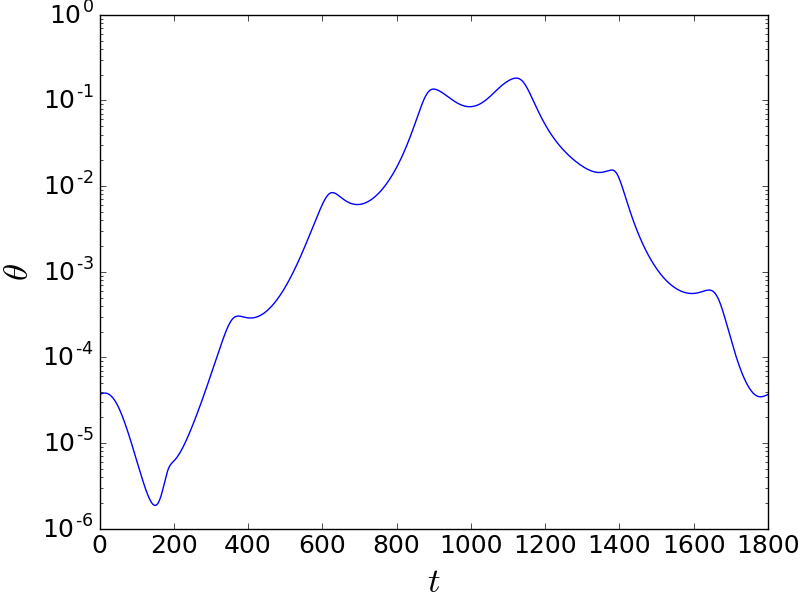
\includegraphics[width=0.46\textwidth]{ks_ppo147_angle}
  (b)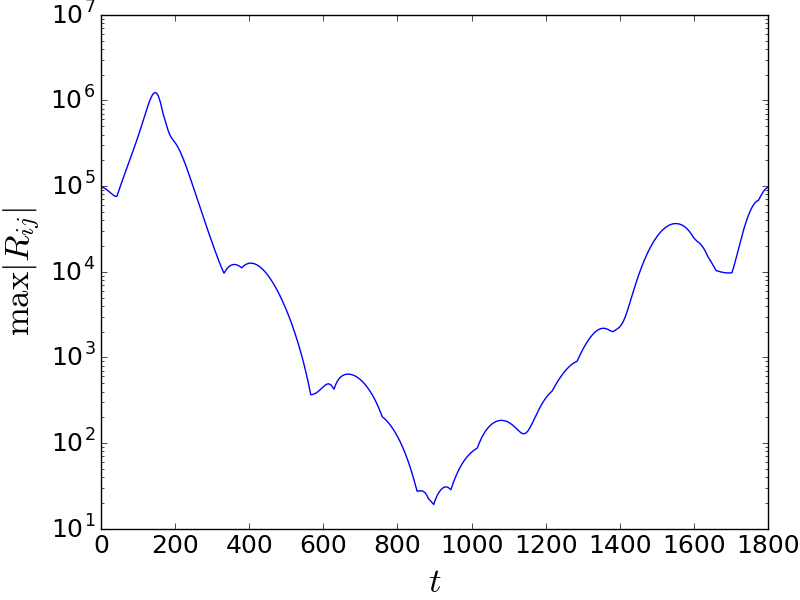
\includegraphics[width=0.46\textwidth]{ks_ppo147_offdiagonal}
  \caption{
    (a) The angle between 1st Floquet vector and the rest. (b)
    the maximal magnitude of the
    off-diagonal element.
  }
  \label{fig:ks_ppo147_offdiagonal}
\end{figure}

\item[2017-02-14 Predrag] to Xiong: Carlo Cossu and Yohann Duguet
tell me that the best reference on linear stability are the two papers
by  Farrell and Ioannou:
{\em Generalized stability theory.
    {Part I: Autonomous} operators}\rf{IoFa69}
and
{\em Generalized stability theory. {
     Part II: Nonautonomous} operators}\rf{IoFa69II}.
I had a glance at the part~I, which emphasizes nonnormality (maybe a
useful reference for that) and part~II, and am not sure that this paper
is so fundamental (it is scholarly - zillion references).

\item[2017-03-4 Xiong]
  I generate spatiotemporal heat plots of the KS system with
  much larger domain $L=100$ and $L=200$ as shown
  in \reffig{fig:KS_LargeL},
  which will be used in my thesis.
  \begin{figure}[h]
    \centering
    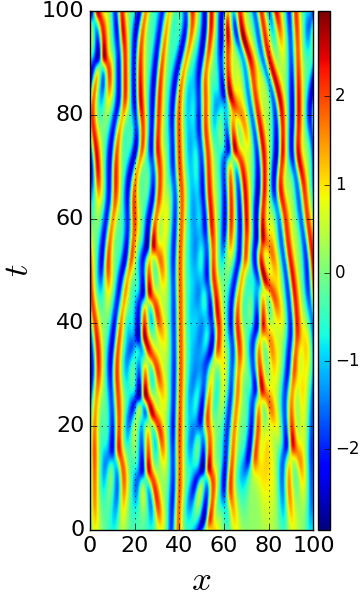
\includegraphics[width=0.36\textwidth]{KS_L100N256}
    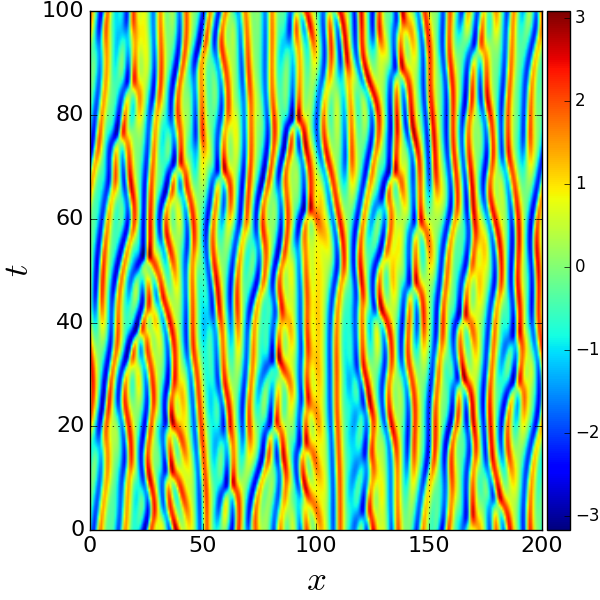
\includegraphics[width=0.6\textwidth]{KS_L200N256}
    \caption{KS using $N=256$ Fourier modes.
      A random initial condition was used.
      Left: $L=100$. Right: $L=200$. }
    \label{fig:KS_LargeL}
  \end{figure}

  Also, I generate spatiotemporal heat plots for the 1d cGL equation,
  $A_t = A + (1 + i\alpha)A_{xx} - (1 +i\beta)|A|^2A$ with
  $\alpha=2$ and $\beta=-2$ shown in \reffig{fig:cGL_LargeL}.
  \begin{figure}[h]
    \centering
    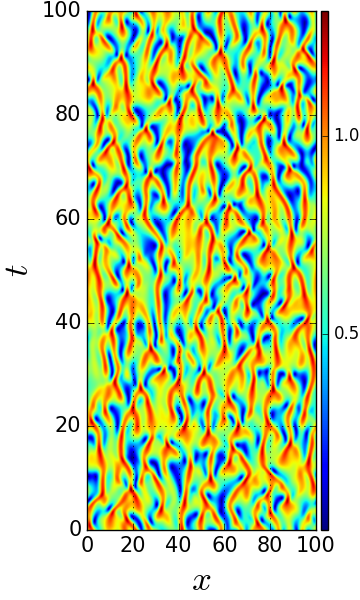
\includegraphics[width=0.36\textwidth]{cGL_L100N256}
    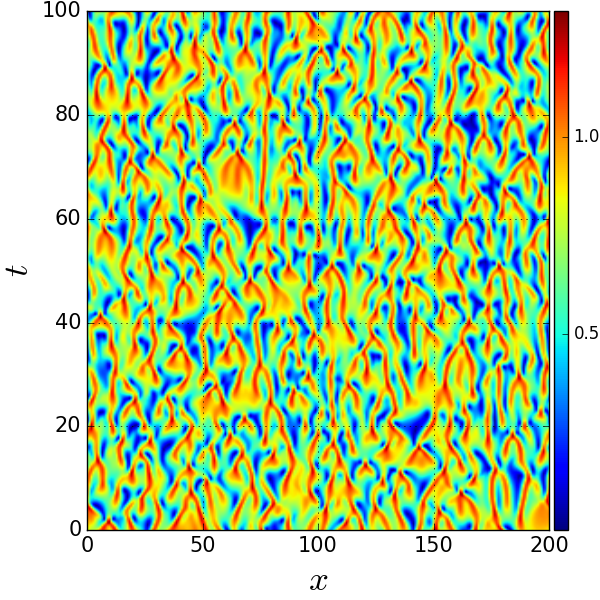
\includegraphics[width=0.6\textwidth]{cGL_L200N256}
    \caption{cGL using $N=256$ Fourier modes.
      A random initial condition was used.
      Left: $L=100$. Right: $L=200$. }
    \label{fig:cGL_LargeL}
  \end{figure}

  I just want to show that in spatially extended chaotic systems,
  the pattern can be studies in a small cell.

\item[2017-03-31 Predrag] Here is a revolutionary idea for
the covariant vectors crowd:

A third of Benjamin Loewe thesis\rf{LoeweThesis,LoHiGo17} is about
Classical Mechanics helping out Quantum Mechanics, in the problem of
``transitionless quantum driving''\rf{Berry09}, so why not go for the
broke, and do something revolutionary?

I think that the adiabatic thinking might be old fashioned, remnant of
Michael Berry era where everything had to be written down as analytical
formulas. Now, when actual computations are always numerical, there is a
better and simpler way:

\begin{enumerate}
  \item Time independent Schr\"odinger equation is equivalent to stability
of an equilibrium of a dynamical system. Its eigenfunctions have meaning
only for an equilibrium (a time invariant Hamiltonian), not for a general
(time driven) trajectory. For real problems in physics and chemistry, the
Hamiltonian is expressed in finite-dimensional functional basis. So is
the stability matrix of a problem such as Navier-Stokes.
  \item If the system is periodically driven, one cannot use
weakly perturbed eigenfunctions of an (instantaneous) Hamiltonian, and
evolve them adiabatically and perturbatively for one driving period, one must
use Floquet eigenfunctions. They have no relation to any instantaneous
stability matrix / Hamiltonian, and they are
certainly not adiabatically related to such set of eigenfunctions.
For real problems in physics and chemistry, the
evolution operator is expressed in finite-dimensional functional basis. So is
the Floquet (Jacobian) matrix of a problem such as Navier-Stokes.
  \item If the external driving is ergodic (evolution does not ever bring
the Hamiltonian operator to a previous form) one can still compute
eigenfunctions as covariant vectors.  For dynamical systems, that is
what Xiong Ding's thesis\rf{DingThesis} is about.
But Quantum Mechanics would require a bit of thinking; there is no
Oseledec dominance in this case, all eigenfunctions are unitary. I
believe that the modern algorithms\rf{GiChLiPo12} for computing
stability (covariant) vectors do not rely on the Oseledec dominance.
\end{enumerate}

\item[2017-04-11 Predrag]
Luca Dieci feels we should have cited \refref{DJRV07} {\em Error in
approximation of {Lyapunov} exponents on inertial manifolds: {The
Kuramoto-Sivashinsky} equation} in our \refrefs{DCTSCD14,DingThesis}, in
particular because they also find that \KS\ inertial manifold dimension
is 8 (see 17 lines above their Eq.~(6.5)).

\HREF{http://people.ku.edu/~erikvv/software_les.html}
{people.ku.edu/~erikvv/software\_les.html}
\\  has
LESLIS/LESLIL and LESNLS/LESNLL Fortran codes for computation of Lyapunov
exponents

\item[2017-05-02 Predrag]                               \inCB
Liebermann, Main and Wunner\rf{LiMaWu17}
{\em Exceptional points in the elliptical three-disk scatterer using
semiclassical periodic orbit quantization}: ``
An interesting general feature of open quantum systems described by
non-Hermitian operators is the possible existence of exceptional points where

\emph{not only the complex eigenvalues but also their respective eigenvectors
coincide.}

We show that exceptional points exist in a three-disk scatterer if
the system's geometry is modified by extending the system from circular to
elliptical disks. The extension is implemented in such a way that the
system's characteristic $C_{3\mathrm{v}}$ symmetry is preserved. The
two-dimensional parameter plane of the system is then spanned by the distance
between and the excentricity of the elliptical disks. As typical signatures
of exceptional points we observe the permutation of two resonances when an
exceptional point is encircled in parameter space, and a non-Lorentzian
resonance line shape in the weighted density of states.
''

An interesting feature of open quantum systems is the possible existence of
exceptional points (EPs)\rf{Moiseyev11,Kato80,Heiss99,Heiss04,Heiss12}.
Contrary  to  Hermitian  systems where in case of degeneracy only the
eigenvalues coincide, in a non-Hermitian system the respective eigenstates
also coalesce at an EP.
To observe EPs,  there have to be at least two real-valued free parameters.

The simplest system with an EP is the two-dimensional matrix
\begin{equation}
  H(\lambda) = \begin{pmatrix}
    1 & \lambda\\
    \lambda & -1
  \end{pmatrix}
\end{equation}
that depends on a complex parameter~$\lambda$~\cite{Kato80}. The matrix is
non-Hermitian for non-real~$\lambda$. The eigenvalues are given by
$\epsilon_1 = \sqrt{1+\lambda^2}$ and $\epsilon_2 = -\sqrt{1+\lambda^2}$.
They become degenerate for $\lambda_0 = {\pm \ii}$. The same holds true for
the respective eigenvectors. Therefore, $\lambda_0$ is an EP. One of the most
striking features of an EP can be observed when the EP is encircled in
parameter space, \emph{e.\,g.} $\lambda(\phi) = \ii + r \exp(\ii\phi)$ for
$\phi = 0 \dots 2\pi$. The eigenvalues in a power-series expansion are then
given by $\epsilon_1 = \sqrt{2r} \exp\bigl[\ii (\pi/4 + \phi/2)\bigr]$ and
$\epsilon_2 = \sqrt{2r} \exp\bigl[\ii (5\pi/4 + \phi/2)\bigr]$. One can see
that for small encircling radii~$r$ the eigenvalues interchange their
positions when the EP is encircled in a closed loop in parameter space. The
EP has to be encircled twice to make the resonances return to their original
positions. However, the respective eigenvectors pick up an additional phase
of~$\pi$. This is a characteristic feature of an EP and will be used as a
distinct identifier for an EP in the elliptical three-disk scatterer.

\item[2017-05-02 Predrag]
Heiss\rf{Heiss99} writes:
``Avoided level crossings are associated with exceptional points which are
the singularities of the spectrum and eigenfunctions, when considered as
functions of a complex coupling parameter. It is shown that the wave function
of one state changes sign but not the other, if the exceptional point is
encircled in the complex plane. An experimental setup is suggested where this
peculiar phase change could be observed.''

Heiss\rf{Heiss04} writes:
``Exceptional points associated with non-Hermitian operators, i.e. operators
being non-Hermitian for real parameter values, are investigated. The specific
characteristics of the eigenfunctions at the exceptional point are worked
out. Within the domain of real parameters the exceptional points are the
points where eigenvalues switch from real to complex values. These and other
results are exemplified by a classical problem leading to exceptional points
of a non-Hermitian matrix.''

Heiss\rf{Heiss12} writes:
``... about the nature of exceptional points (EPs) followed by discussions
about their ubiquitous occurrence in a great variety of physical problems.
EPs feature in classical as well as in quantum mechanical problems. They are
associated with symmetry breaking for {${\mathcal P}{\mathcal T}$}-symmetric
Hamiltonians. EPs are involved in quantum phase transition and quantum chaos;
they produce dramatic effects in multichannel scattering, specific time
dependence and more. In nuclear physics, they are associated with
instabilities and continuum problems. Being spectral singularities they also
affect approximation schemes. This article is part of a special issue of
\emph{J. Phys. A} devoted to `Quantum physics with non-Hermitian
operators'.''

\PCpost{2017-06-13}{
Mike Schatz told us in February to look at
Xu and Paul\rf{XuPaul16}
{\em Covariant {Lyapunov} vectors of chaotic {Rayleigh-B{\'e}nard} convection}.
We really should.
}

\PCpost{2019-05-11}{
Carlu, Ginelli, Lucarini and Politi\rf{CGLP19} {\em Lyapunov analysis of
multiscale dynamics: the slow bundle of the two-scale {Lorenz} 96 model}:

[...] study of the full spectrum of covariant Lyapunov vectors reveals the
presence of a slow bundle in tangent space, composed by a set of vectors
with a significant projection onto the slow degrees of freedom; they
correspond to the smallest (in absolute value) Lyapunov exponents and
thereby to the longer timescales. [...] the dimension of the slow
bundle is extensive in the number of both slow and fast degrees of
freedom [...] the conjecture [is] that the
slow-variable behavior is determined by a subset
of degrees of freedom [...:] the slow bundle
corresponds to the Lyapunov spectrum region where fast and slow
instability rates overlap, ``mixing'' their evolution into a set of vectors
which simultaneously carry information on both scales.

[...] a variety of scales makes it hard to approach such systems using
direct numerical integrations, since the problem is stiff.

[...] in the limit of an infinite timescale separation between the slow
modes of interest and the very fast degrees of freedom [...]  the
homogenization theory [...] the effect of the fast degrees of freedom can
be written as the sum of a deterministic, drift-like correction plus a
stochastic white-noise forcing\rf{PavStu08}.

[...] difficulty in the study of the multiscale nature of the climate
system comes from the lack of any well-defined separation of scales
(spectral gap).

Mori-Zwanzig and Ruelle response theory\rf{WouLuc13}.

[...] in the absence of forcing and dissipation [...] a quadratic form of
slow and fast variables [...] is conserved\rf{VisLuc17} [...] suggesting
that E can be identified with energy - and represents a natural norm –
also in the forced and dissipative case.

Spatially extended systems [...] exhibit an extensive Lyapunov
spectrum\rf{ruelle,ruelext,LiPoRu86,Grassberger89}. This property is
instrumental for the identification of intensive and extensive
observables in the thermodynamic sense. Extensivity means that for $N$
tending to infinity (\ie, in the so-called thermodynamic limit), the
spectrum $\{\lambda_i\}$ is a function of the rescaled index $\rho=i/N$
only. Their Fig.~1 illustrates the extensivity of chaos very nicely.

The Kolmogorov–Sinai entropy $H_{KS}$ - a measure of the diversity of the
trajectories generated by the dynamical system - and the Kaplan–Yorke
dimension $D_{KS}$ are proportional to the number $N$ of degrees of
freedom.

[...] the energy conservation law in the zero-dissipation limit accounts
for the existence of an extra zero-Lyapunov exponent [...] but the
Lyapunov spectrum [...] is perfectly symmetric, as the second half of the
spectrum superposes to the first half under the transformation
$\lambda_i\to-\lambda_{N-i+1}$. [...] this model is known to possess no
symplectic structure, and [...] the overall symmetry remains an
unexplained property.

[...] the slow bundle extends in tangent space over roughly 120 CLVs,
much more than the $K=36$ slow degrees of freedom.

[...] The slow bundle
[...] does not coincide with the slow variables themselves but involves also
a finite fraction of the fast ones, singling out a fundamental set of
tangent-space perturbations closely associated with the slow dynamics.
[...] the origin of the slow bundle can be traced back to a sort of
resonance between the slow variables and a suitable subset of the fast
ones.
[...] Fluctuations are the unavoidable consequence of the different
degrees of stability experienced in different regions of the phase space,
and they occur in both strictly hyperbolic and nonhyperbolic dynamical
systems, although they are typically much larger in the latter context.
[...] Fluctuations may be so large as to bridge the gap between distinct LEs,
which results in a lack of domination of the Oseledets splitting
[...] and in the sporadic occurrence of near tangencies between pairs of
different CLVs.
[...] the corresponding CLVs are characterized by nonnegligible near
tangencies: The probability distribution of the relative angle, [...]
exhibits a peak near 0.
[...] The near tangencies between different CLVs within the slow bundle
provide numerical evidence of the mixing between slow and fast
degrees of freedom.
[...] the large ratio between the amplitude of the fluctuations and the
separation between consecutive LEs suggests that this exchange of
directions may extend beyond the nearest neighbors along the spectrum.

[...] As the finite-size Lyapunov exponents (FSLE) depend on the norm, we
[...] study the behavior of an entire family of Euclidean norms.

[...] the linearly controlled growth of small, finite perturbations stops
as soon as the fast components saturate because of nonlinearities.
Afterwards, fast variables act as a sort of noise on the slow ones, whose
dynamics is still in the linear regime.

[...] In the future, we would like to explore whether a data assimilation
scheme restricted to the slow bundle only (which does not encompass the
entire unstable space) can lead to further improvements in forecasting.
}

\end{description}

\renewcommand{\ssp}{a}
